\chapter{Design}

\section{Overall System Design}

\subsection{Short description of the main parts of the system}

\begin{itemize}
    \item Media Inventory Database
    \begin{itemize}
        \item General Interface
        \item Adding Records
        \item Displaying Records
        \item Searching Records
        \item Editing Records
        \item Deleting Records
    \end{itemize}
\end{itemize}

General Interface
\begin{itemize}
    \item The user will be presented with a box whereby he/she will enter a password. This password will be the same for all users who have access to the system.
    \item Once logged in, the user will be confronted with an interface consisting of a series of menu options. These options will be "Add Record", "Display Records", "Search Records", "Edit Record", "Delete Record" and "Change Password".
    \item When the "Change Password" button has been clicked, the user will be taking to a box where they will be required to enter the previous password, then enter a new password twice.
    \item Clicking on the "Add Record" button will take the user to an interface where they will be required to select the type of record they wish to enter.
    \begin{itemize}
        \item Clicking the "Add Loan" button will present an interface to the user where they will have a choice of selecting an existing customer specific loan or creating a new customer specific loan.
        \item Selecting the "Add PAT Test" button will present the user with an interface to choose a PAT test date or to create a new PAT test date.
    \end{itemize}
    \item Clicking on the "Display Records" button will send the user to an interface where they will have to select the table from which table they wish to see the records.
    \item Clicking on the "Edit Records" button will send the user to an interface where they will have to select the table from which they want to edit a record.
    \item Clicking on the "Delete Records" button will send the user to an interface where they will have to select the table from which they wish to delete a record.
\end{itemize}

Adding Information
\begin{itemize}
    \item The system will present the user with a drop down menu from which the user will have to choose an option for which to enter information. After selecting the option, the user will then be presented with a group of data to add to the new record. If any of these options require the user to enter data relating to another table within the database, they will be presented with a drop down menu and will be required to select an option before they record can be created.
    \item Once all the required data fields have been complete, the system will add a unique identifier to the record of information and save in to the database
\end{itemize}

\newpage

Displaying Records
\begin{itemize}
    \item The system will present the user with an interface with a drop down menu, where they will have to select the database  table from which they wan to view the data.
    \item Once the table has been selected, the user will then be presented with a view table that will display all the records within that database  table. They can then choose to sort this information into ascending or descending order by selecting any row for which to sort it by.
\end{itemize}

Editing Records
\begin{itemize}
    \item The system will bring up a user interface that will present a drop down menu where the user will have to select a database table from which they wish to edit a record.
    \item Once a table has been selected, the user will then be confronted with a user interface which will display all the records within that table and then prompt the user to select the record they would like to edit, by enter the unique identifier of this record.
    \item When the record has been selected, the user will be presented with an interface similar to the one where the user enters a new record, but the fields already contain the information. The user will then have to update which field of information to update.
    \item Once data has been updated and a "Done" button has been clicked, the user will then be asked to confirm the updates.
    \item When the updates have been confirmed, the system replace the old record with the new updated record.
\end{itemize}

Deleting Records
\begin{itemize}
    \item The system will present the user with an interface containing a drop down menu where they will have to select a database table from which they wish to delete a record.
    \item After the database table has been selected, the user will be presented with a view table showing all the records within the database table. Underneath the view table will be a prompt, asking the user for the unique identifier of the record they wish to delete.
    \newpage
    \item When the user has selected the record they wish to delete, they will have to confirm this by entering the system password.
    \item The system will then remove the record from the database permanently.
\end{itemize}

\subsection{System flowcharts showing an overview of the complete system}

\begin{figure}[H]
    \begin{center}
        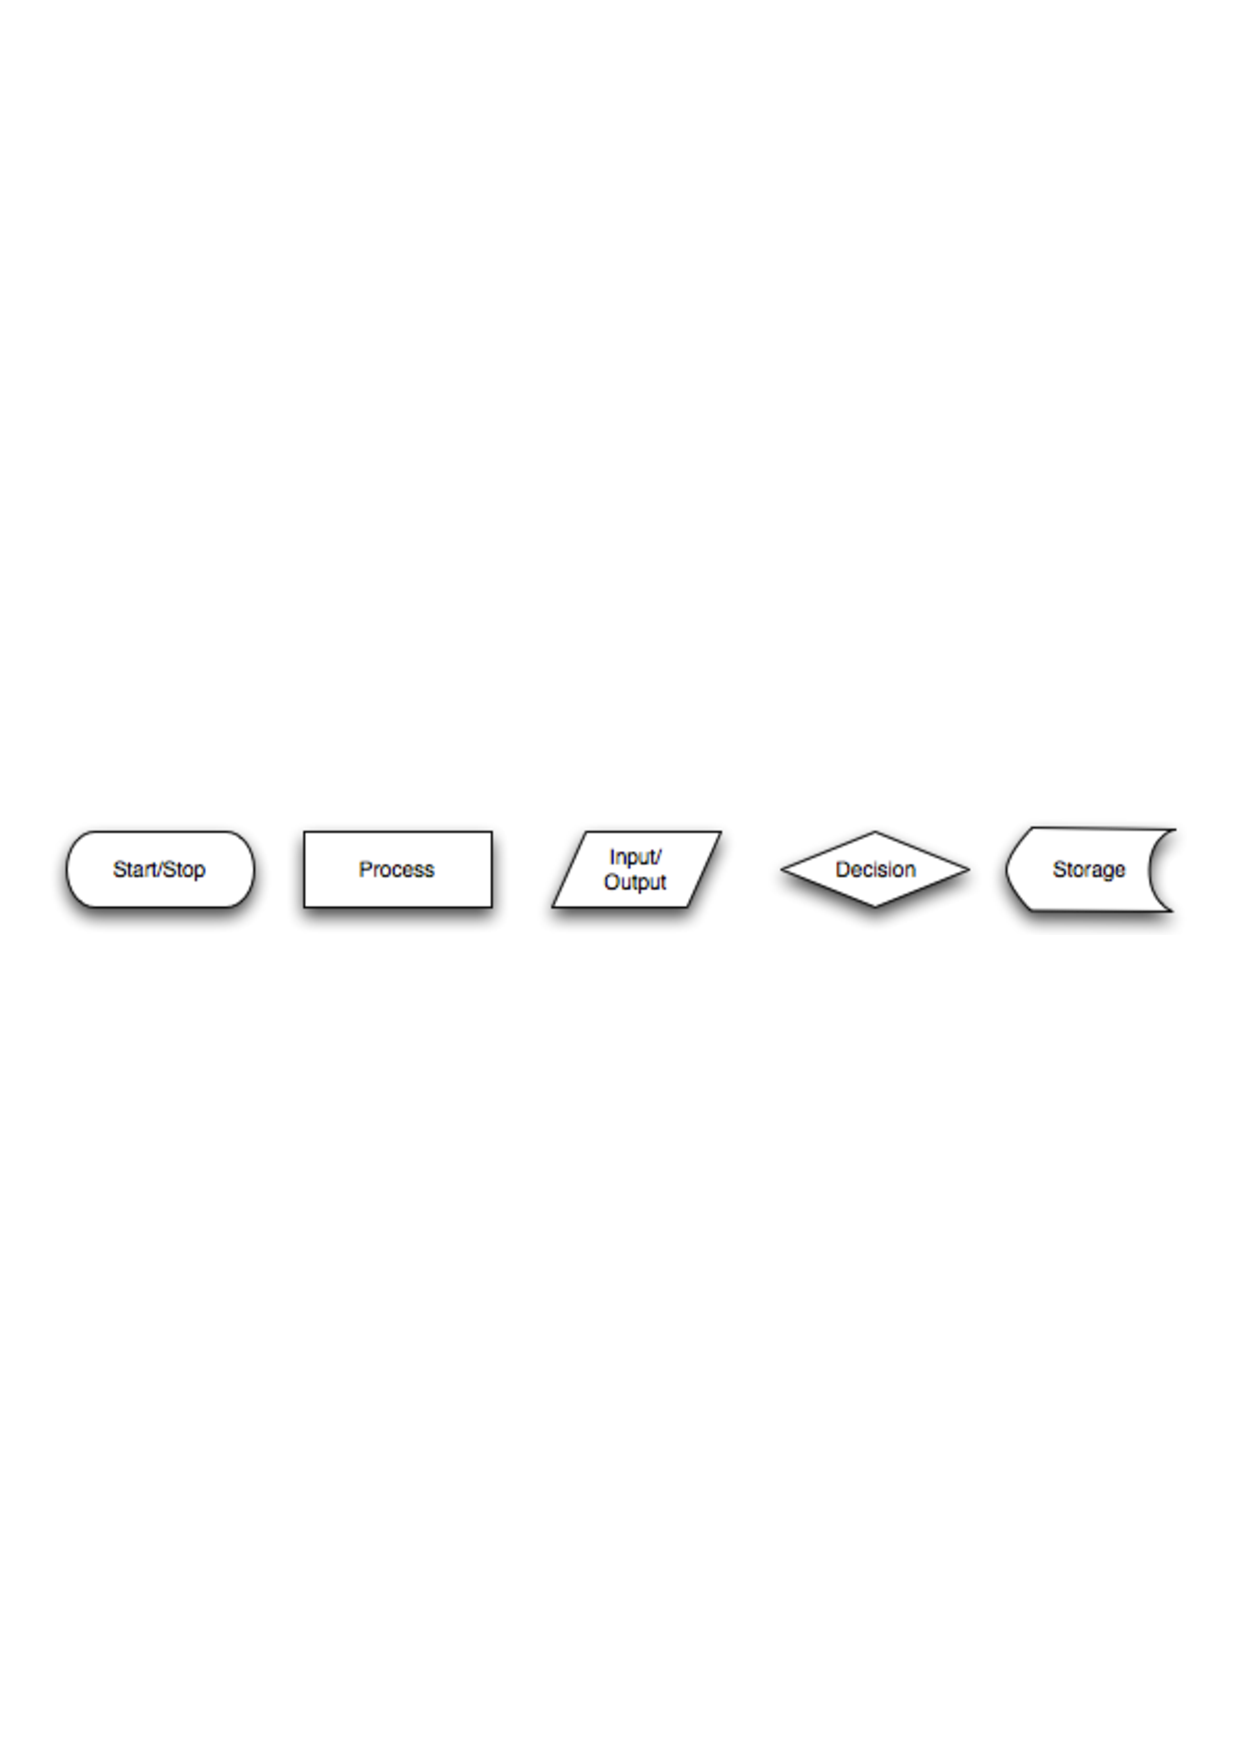
\includegraphics[width=355px]{./Design/system_flowcharts/PDFs/flowchart_key.pdf}
    \end{center}
    \caption{Main System Flowchart.} \label{fig:print_function_result}
\end{figure}

\begin{figure}[H]
    \begin{center}
        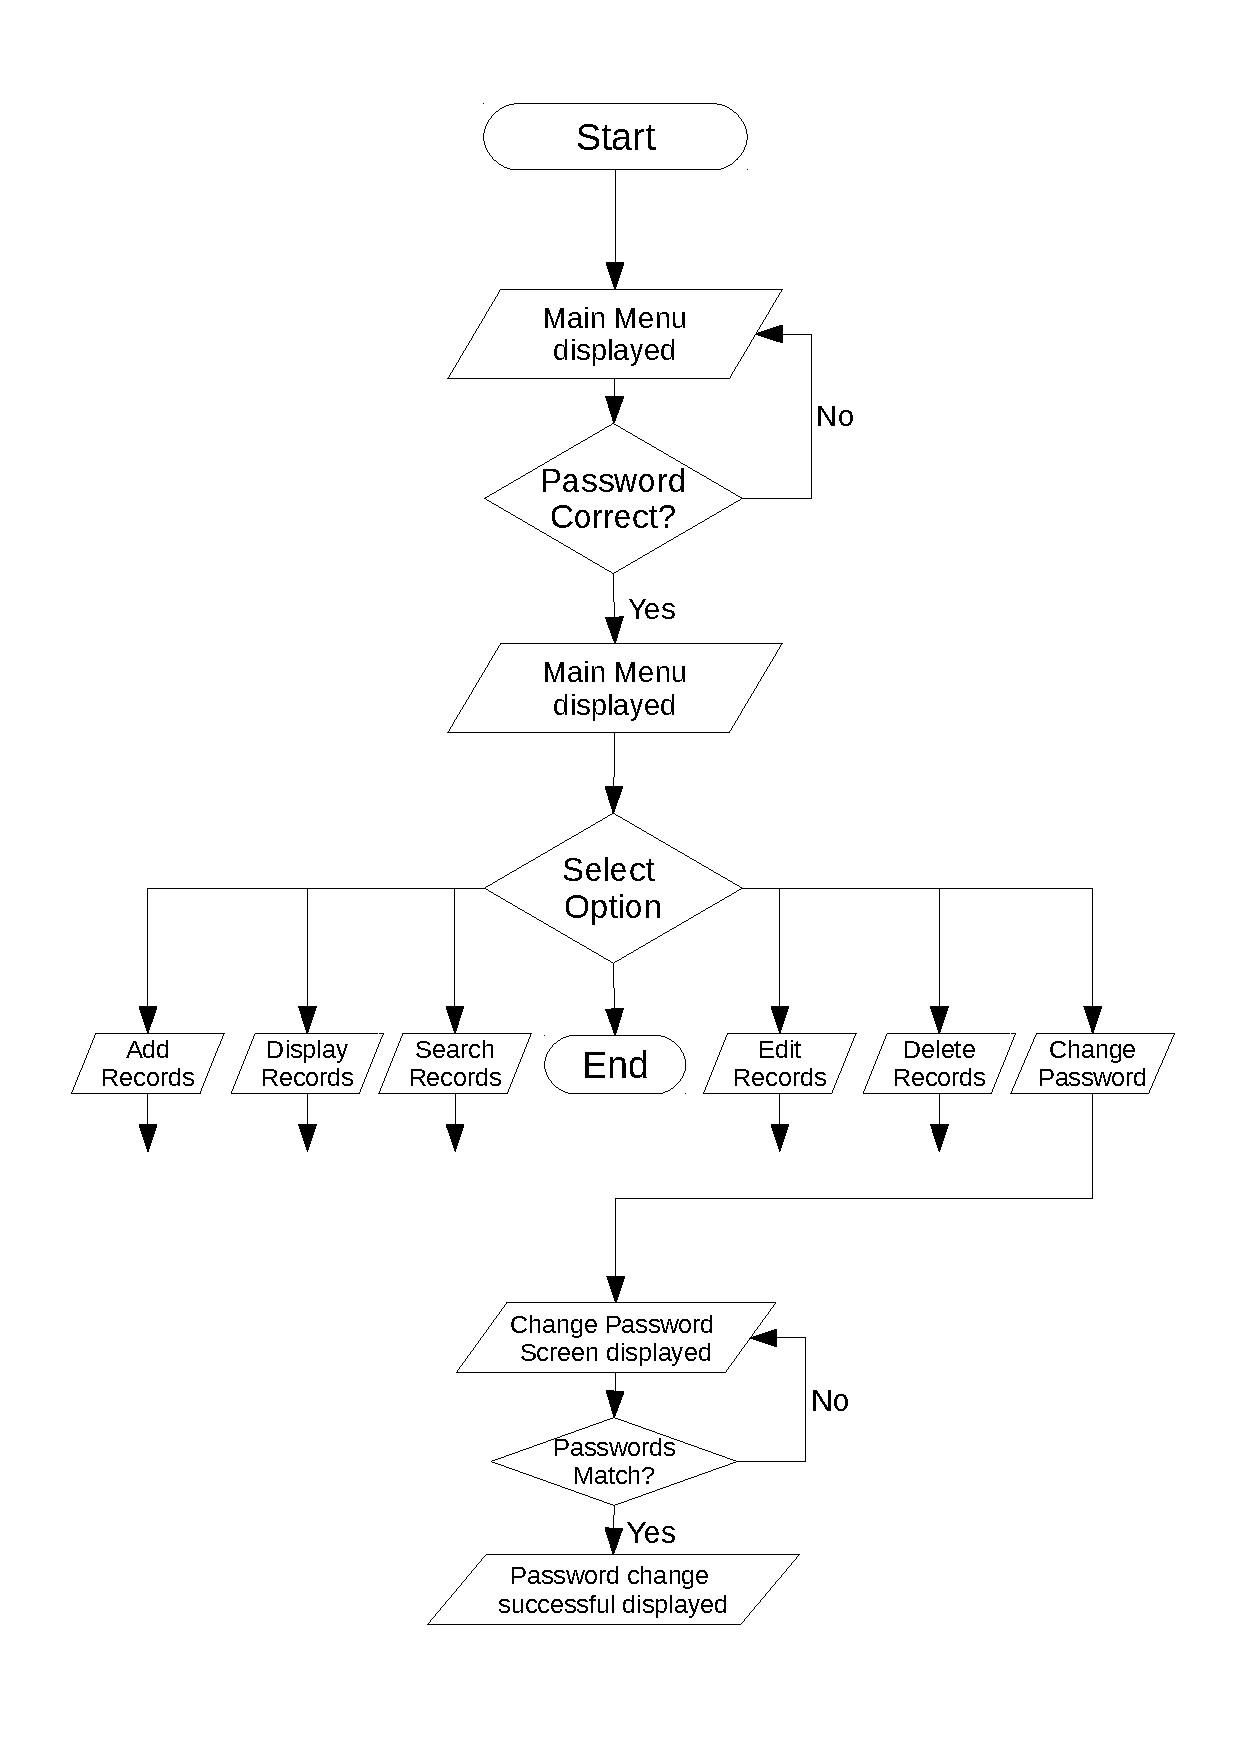
\includegraphics[width=355px]{./Design/system_flowcharts/PDFs/main_system_flowchart.pdf}
    \end{center}
    \caption{Main System Flowchart.} \label{fig:print_function_result}
\end{figure}

\begin{figure}[H]
    \begin{center}
        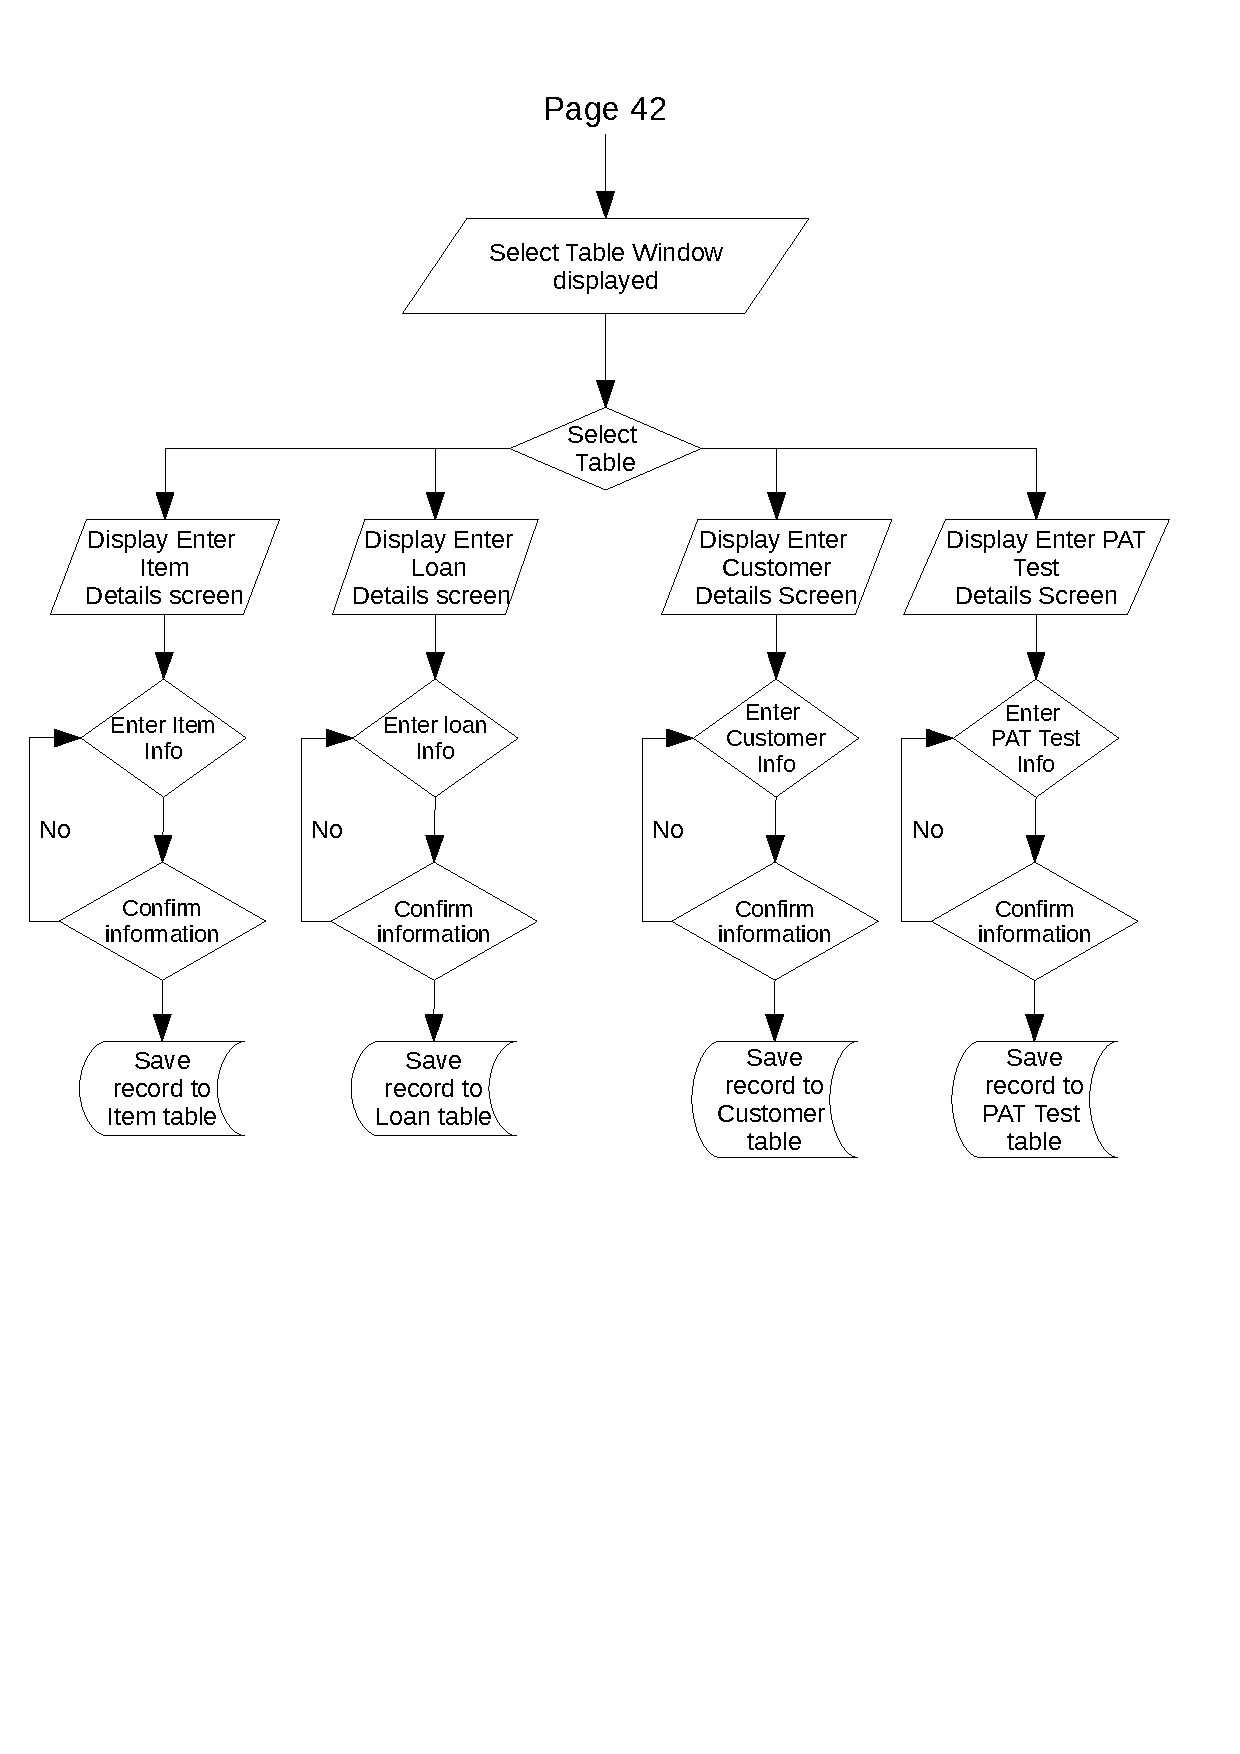
\includegraphics[width=355px]{./Design/system_flowcharts/PDFs/add_records_flowchart.pdf}
    \end{center}
    \caption{Add Records Flowchart.} \label{fig:print_function_result}
\end{figure}

\begin{figure}[H]
    \begin{center}
        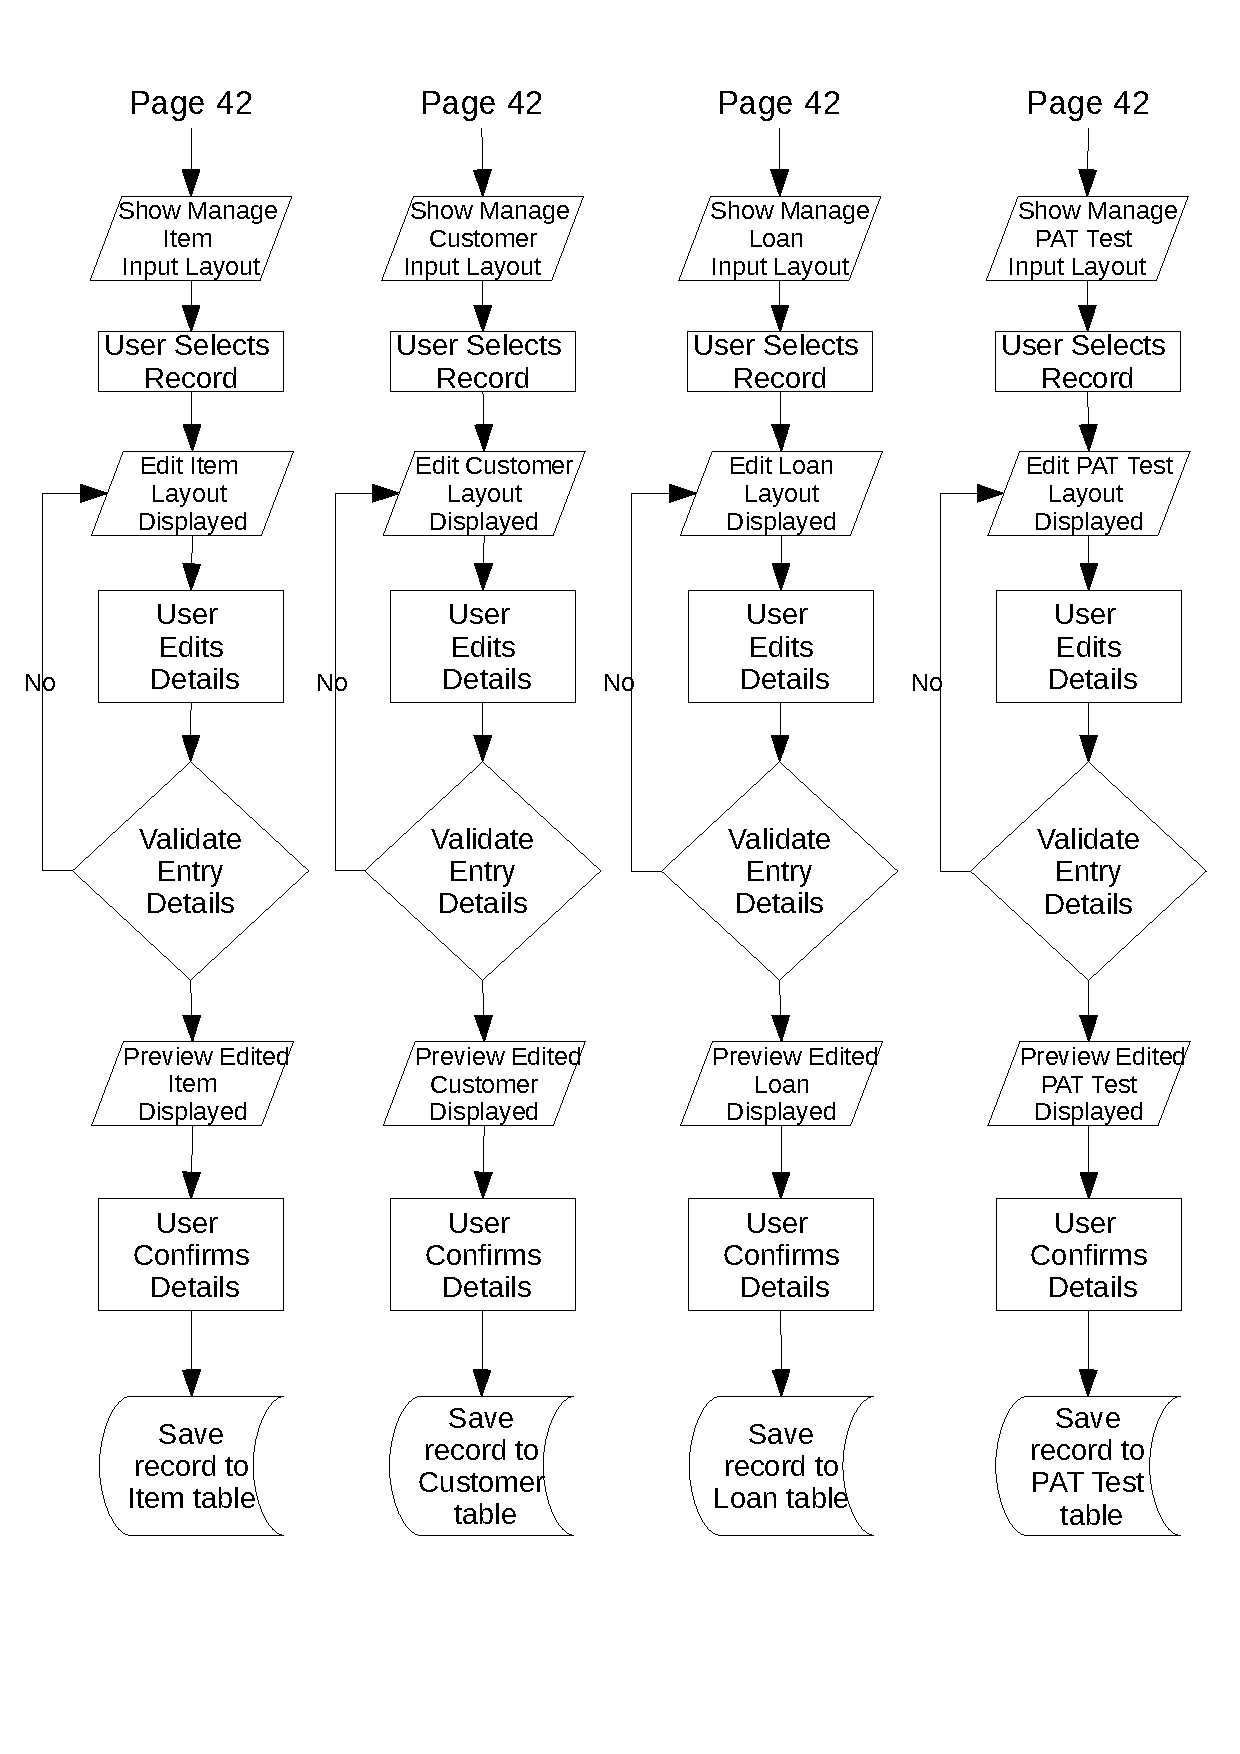
\includegraphics[width=355px]{./Design/system_flowcharts/PDFs/manage_records_flowchart.pdf}
    \end{center}
    \caption{Display Records Flowchart.} \label{fig:print_function_result}
\end{figure}

\begin{landscape}

\section{User Interface Designs}

<<<<<<< HEAD
\begin{figure}[H]
    \begin{center}
        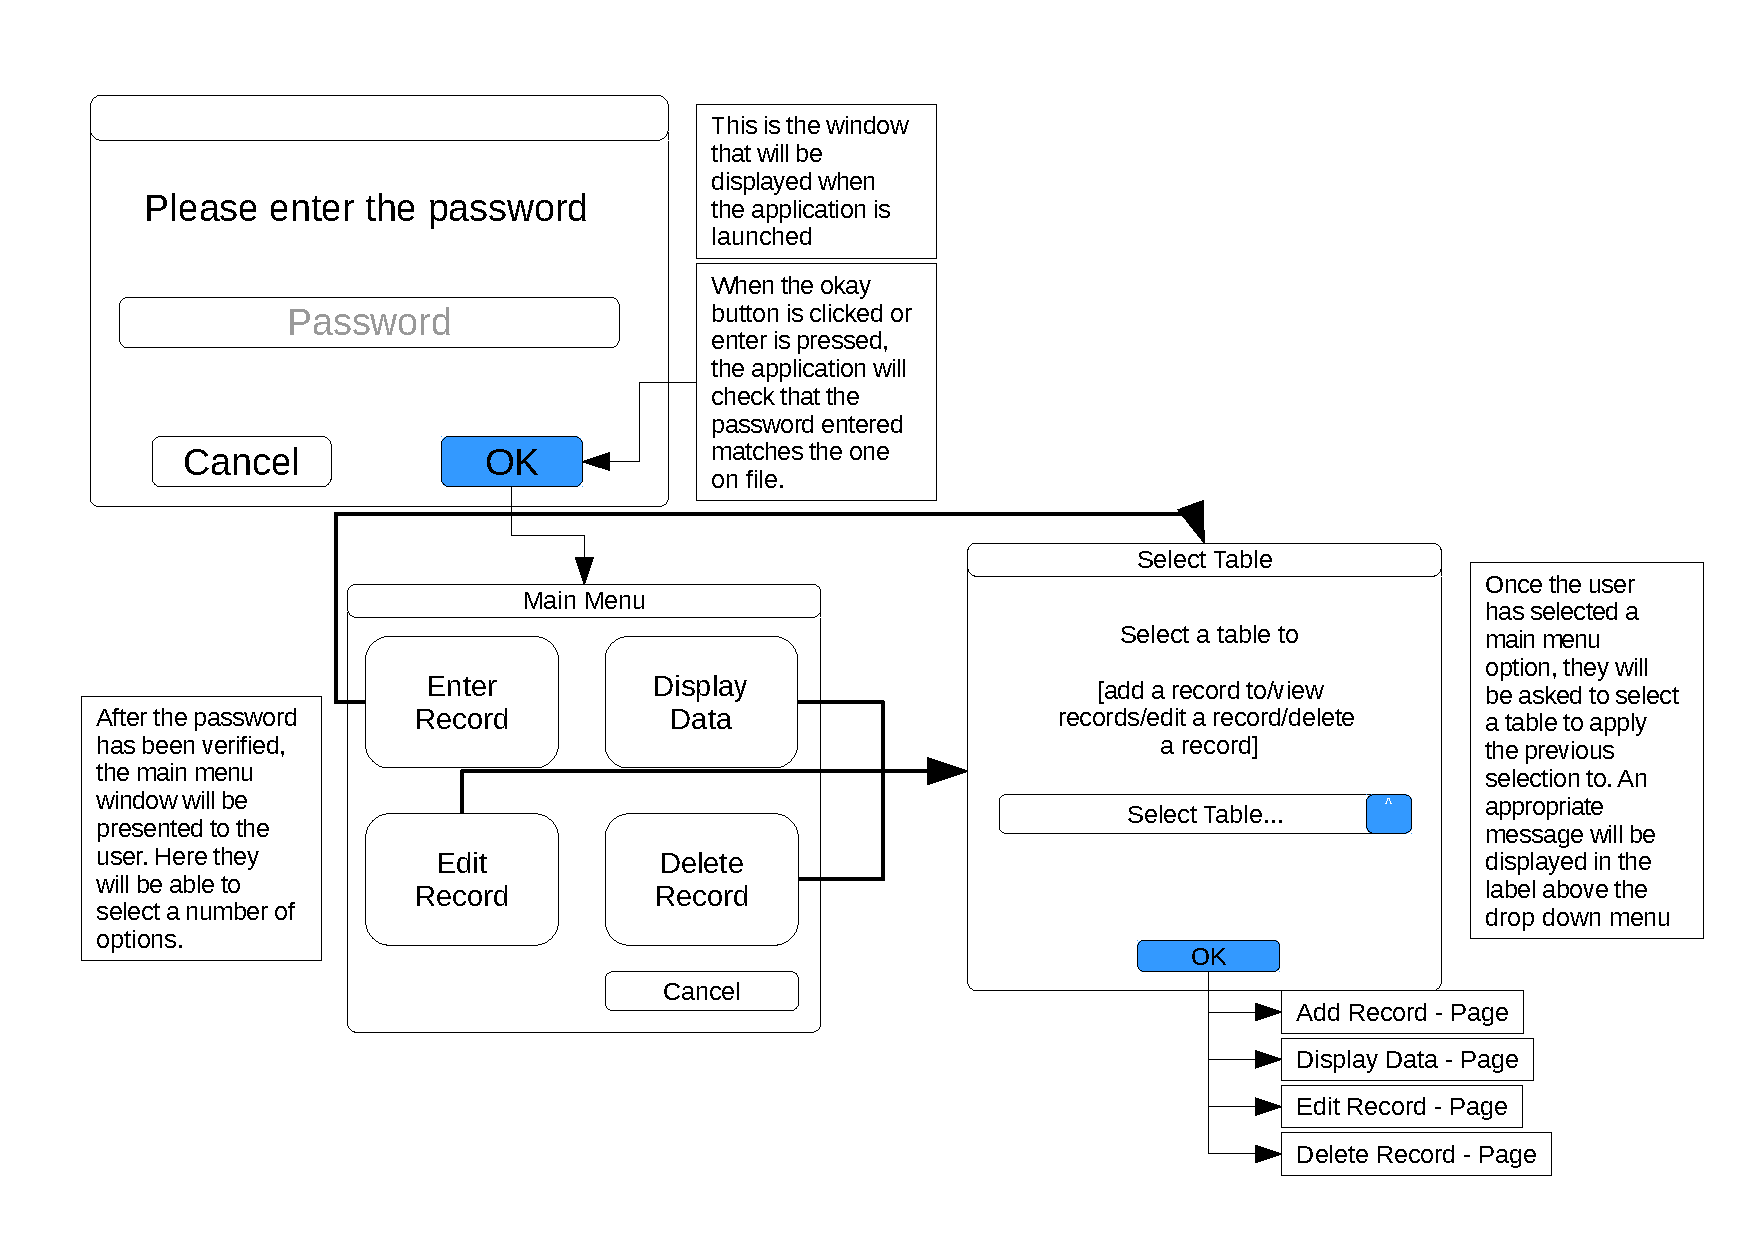
\includegraphics[width=420px]{./Design/user_interface/login_interface.pdf}
    \end{center}
    \caption{Login and Main Menu windows.} \label{fig:print_function_result}
\end{figure}

\begin{center}
    Clicking the "Logout" button will return you to the login screen.
\end{center}

\newpage

\begin{figure}[H]
    \begin{center}
        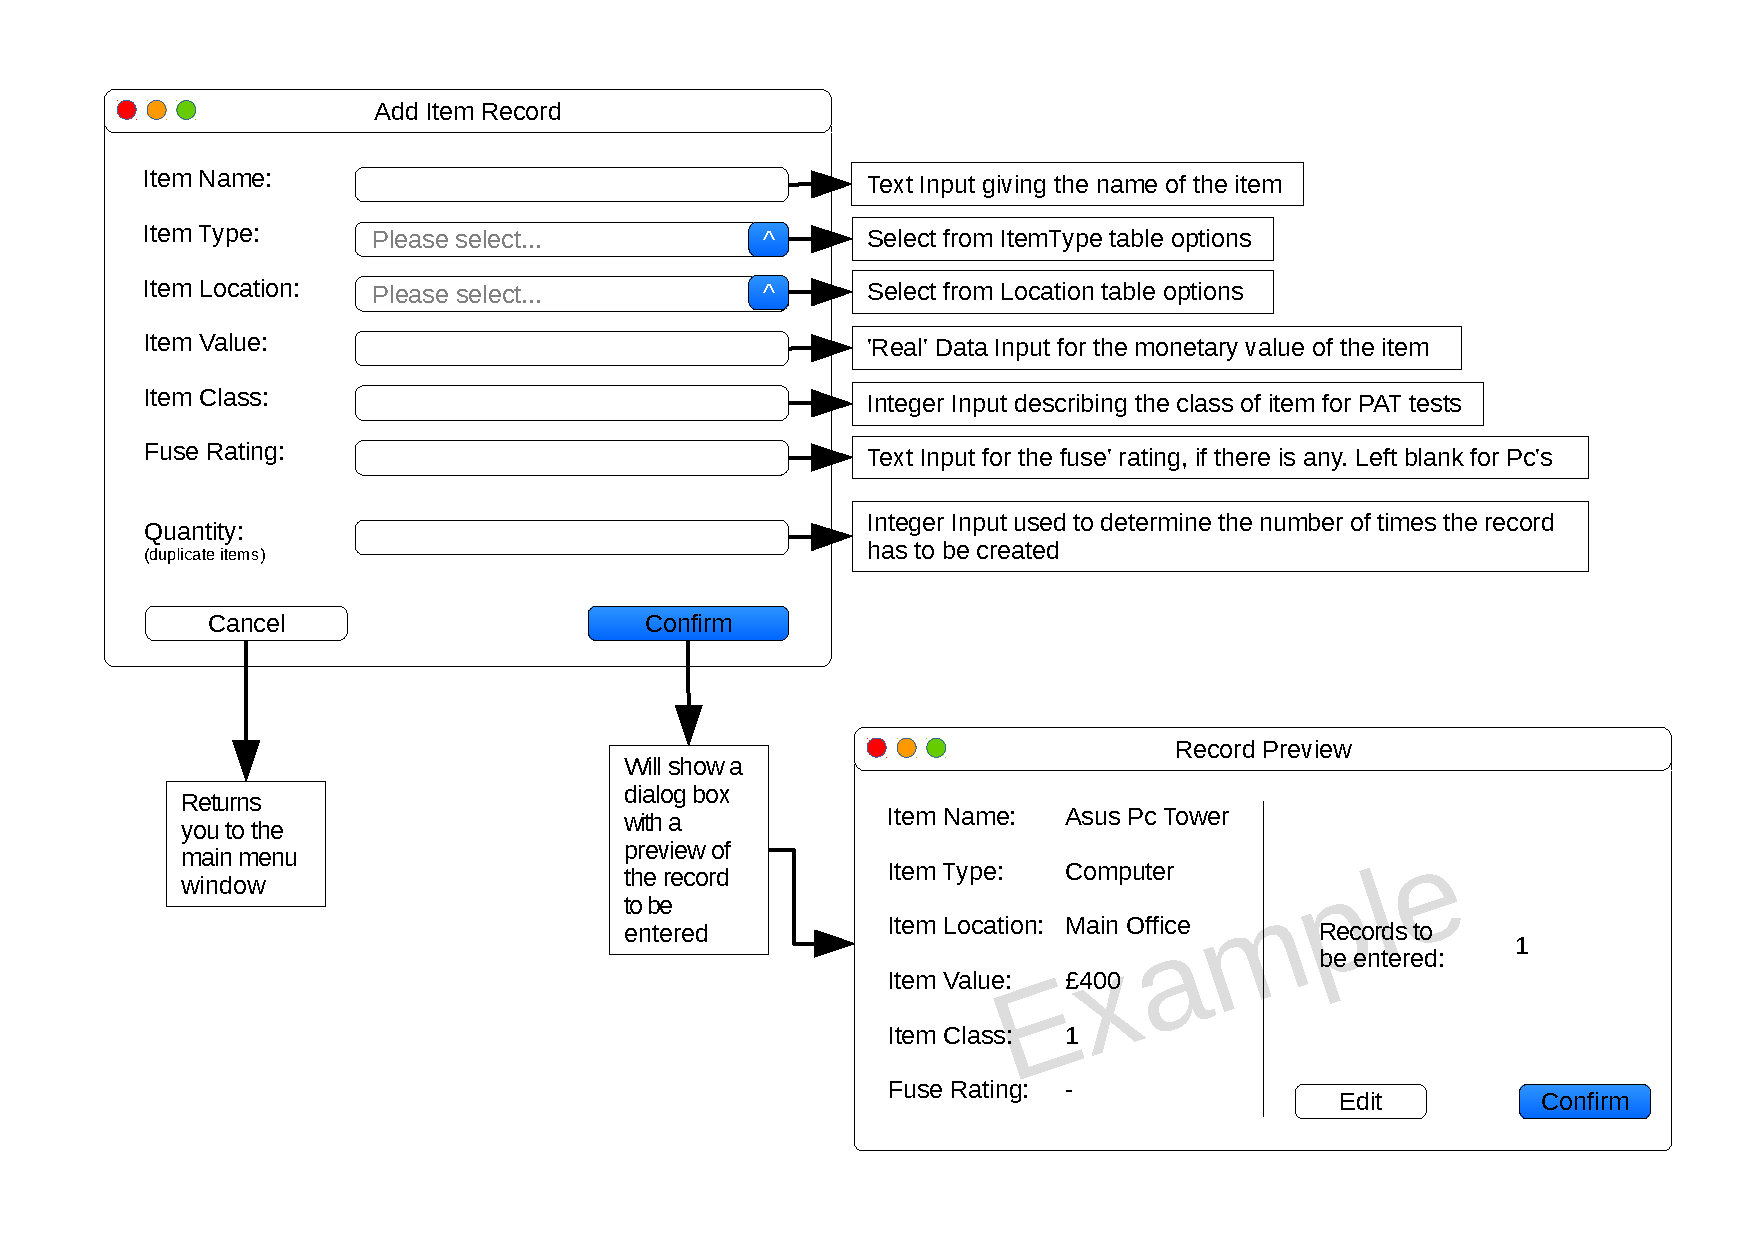
\includegraphics[width=500px]{./Design/user_interface/Add_item_record_interface.pdf}
    \end{center}
    \caption{Login and Main Menu windows.} \label{fig:print_function_result}
\end{figure}

\newpage

\begin{figure}[H]
    \begin{center}
        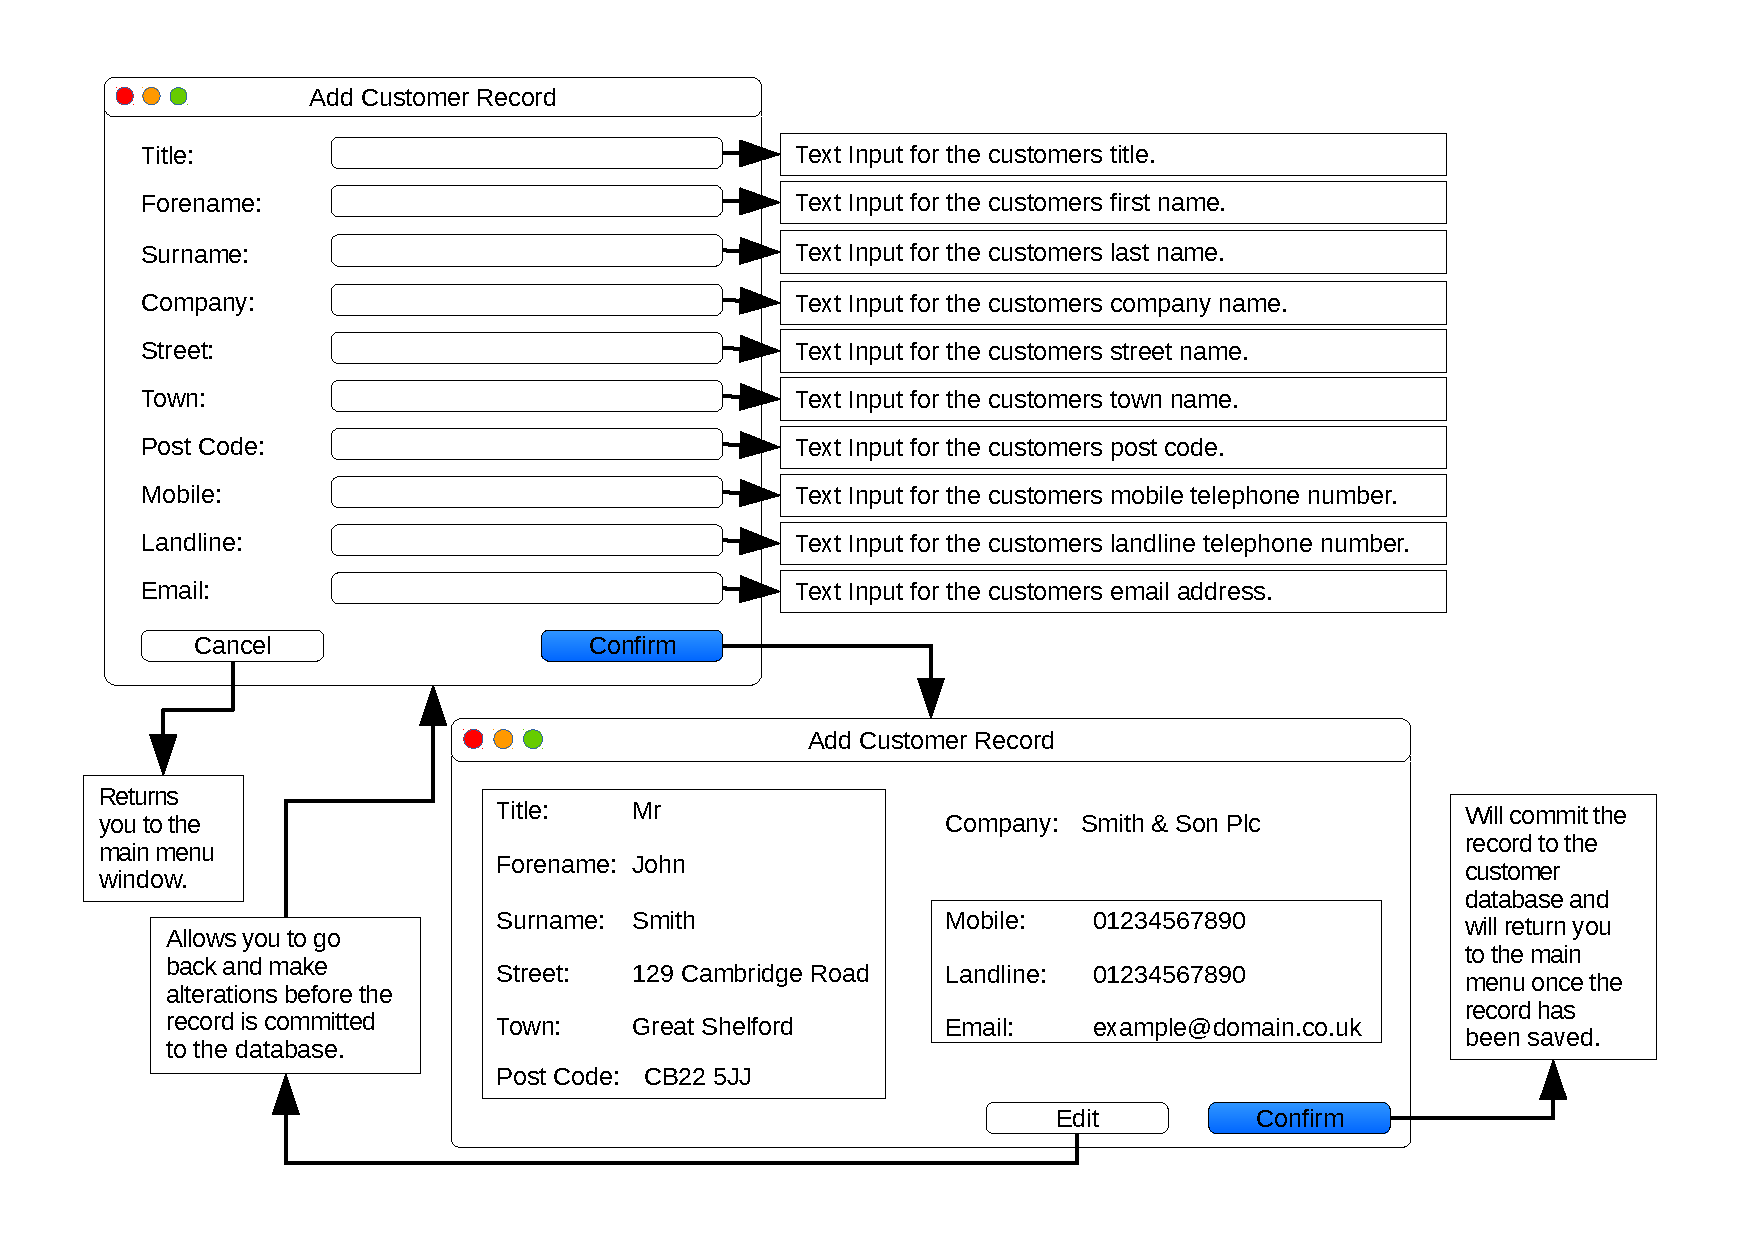
\includegraphics[width=500px]{./Design/user_interface/Add_customer_record_interface.pdf}
    \end{center}
    \caption{Login and Main Menu windows.} \label{fig:print_function_result}
\end{figure}

\newpage

\begin{figure}[H]
    \begin{center}
        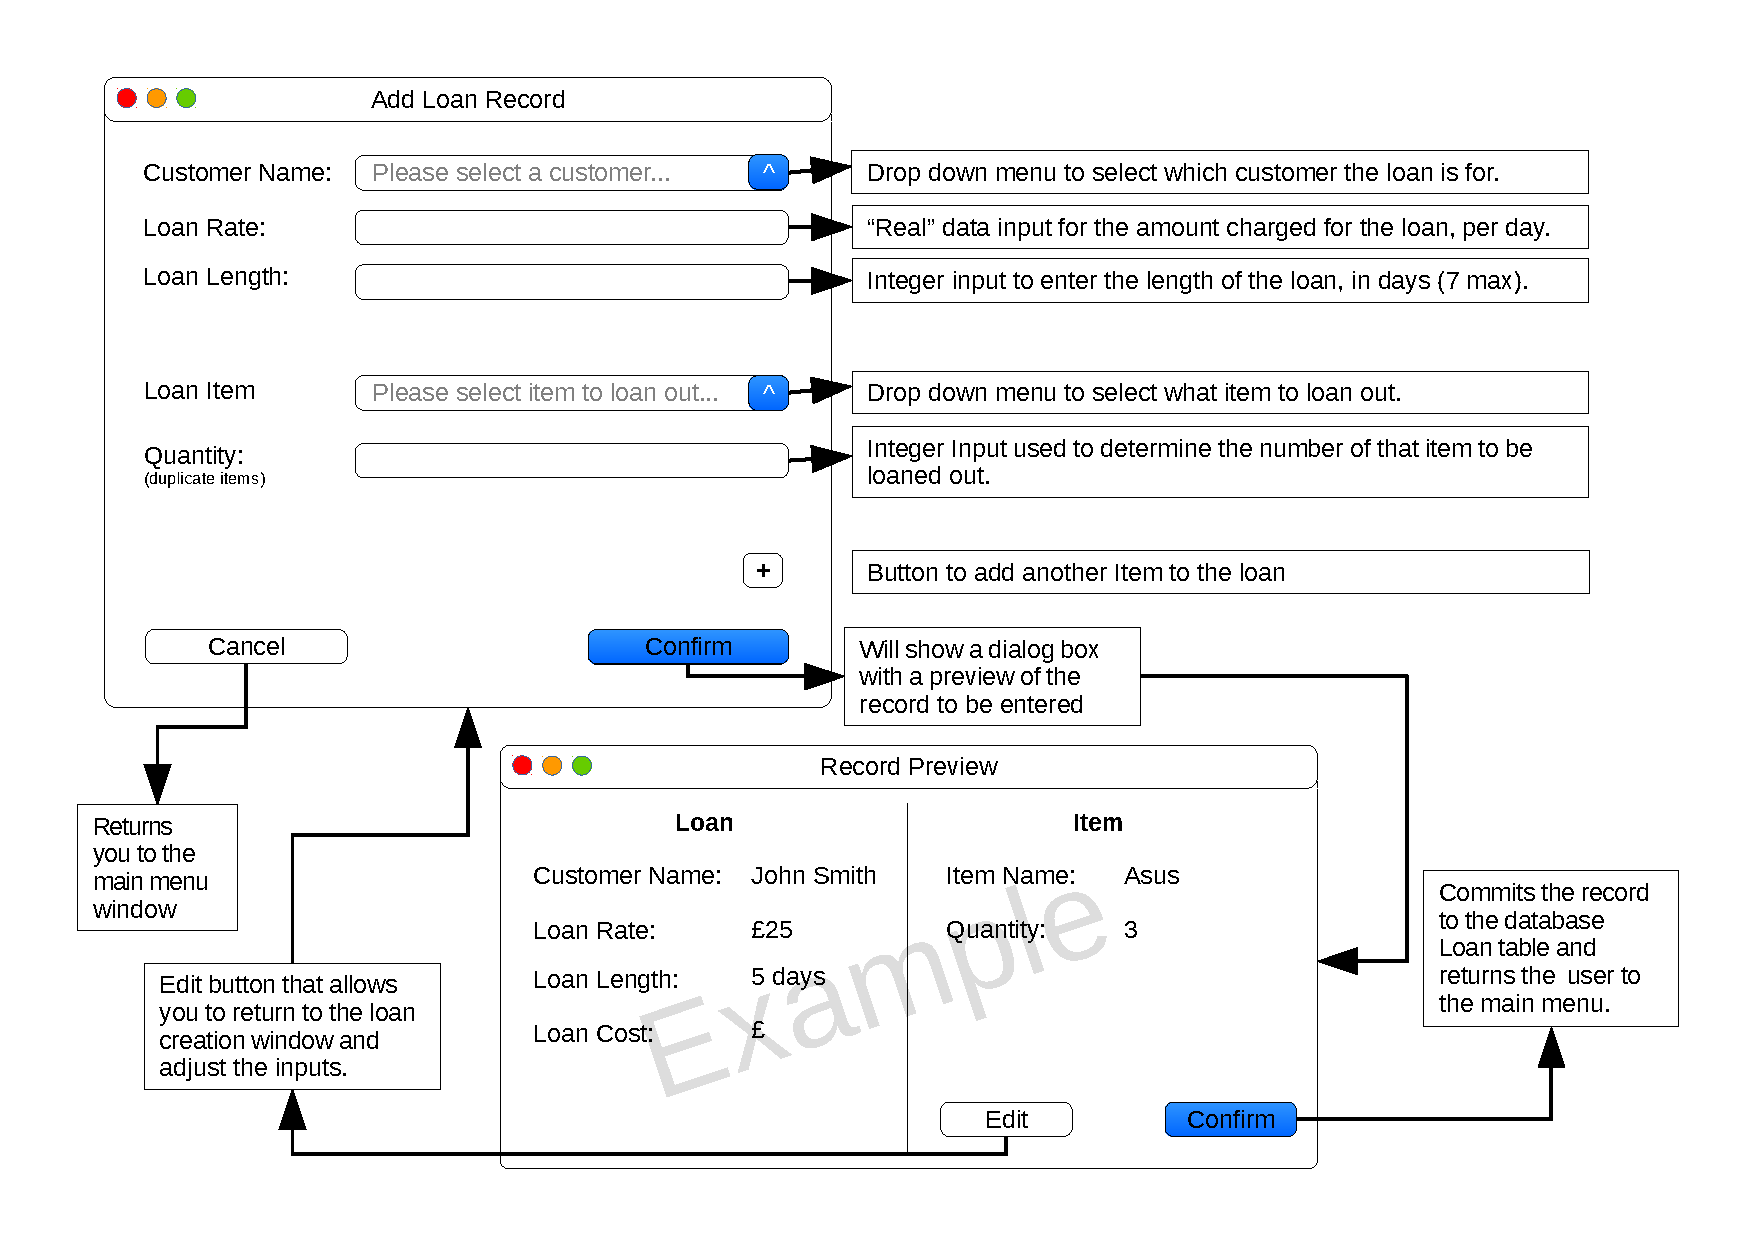
\includegraphics[width=500px]{./Design/user_interface/Add_loan_record_interface.pdf}
    \end{center}
    \caption{Login and Main Menu windows.} \label{fig:print_function_result}
\end{figure}

\newpage

\begin{figure}[H]
    \begin{center}
        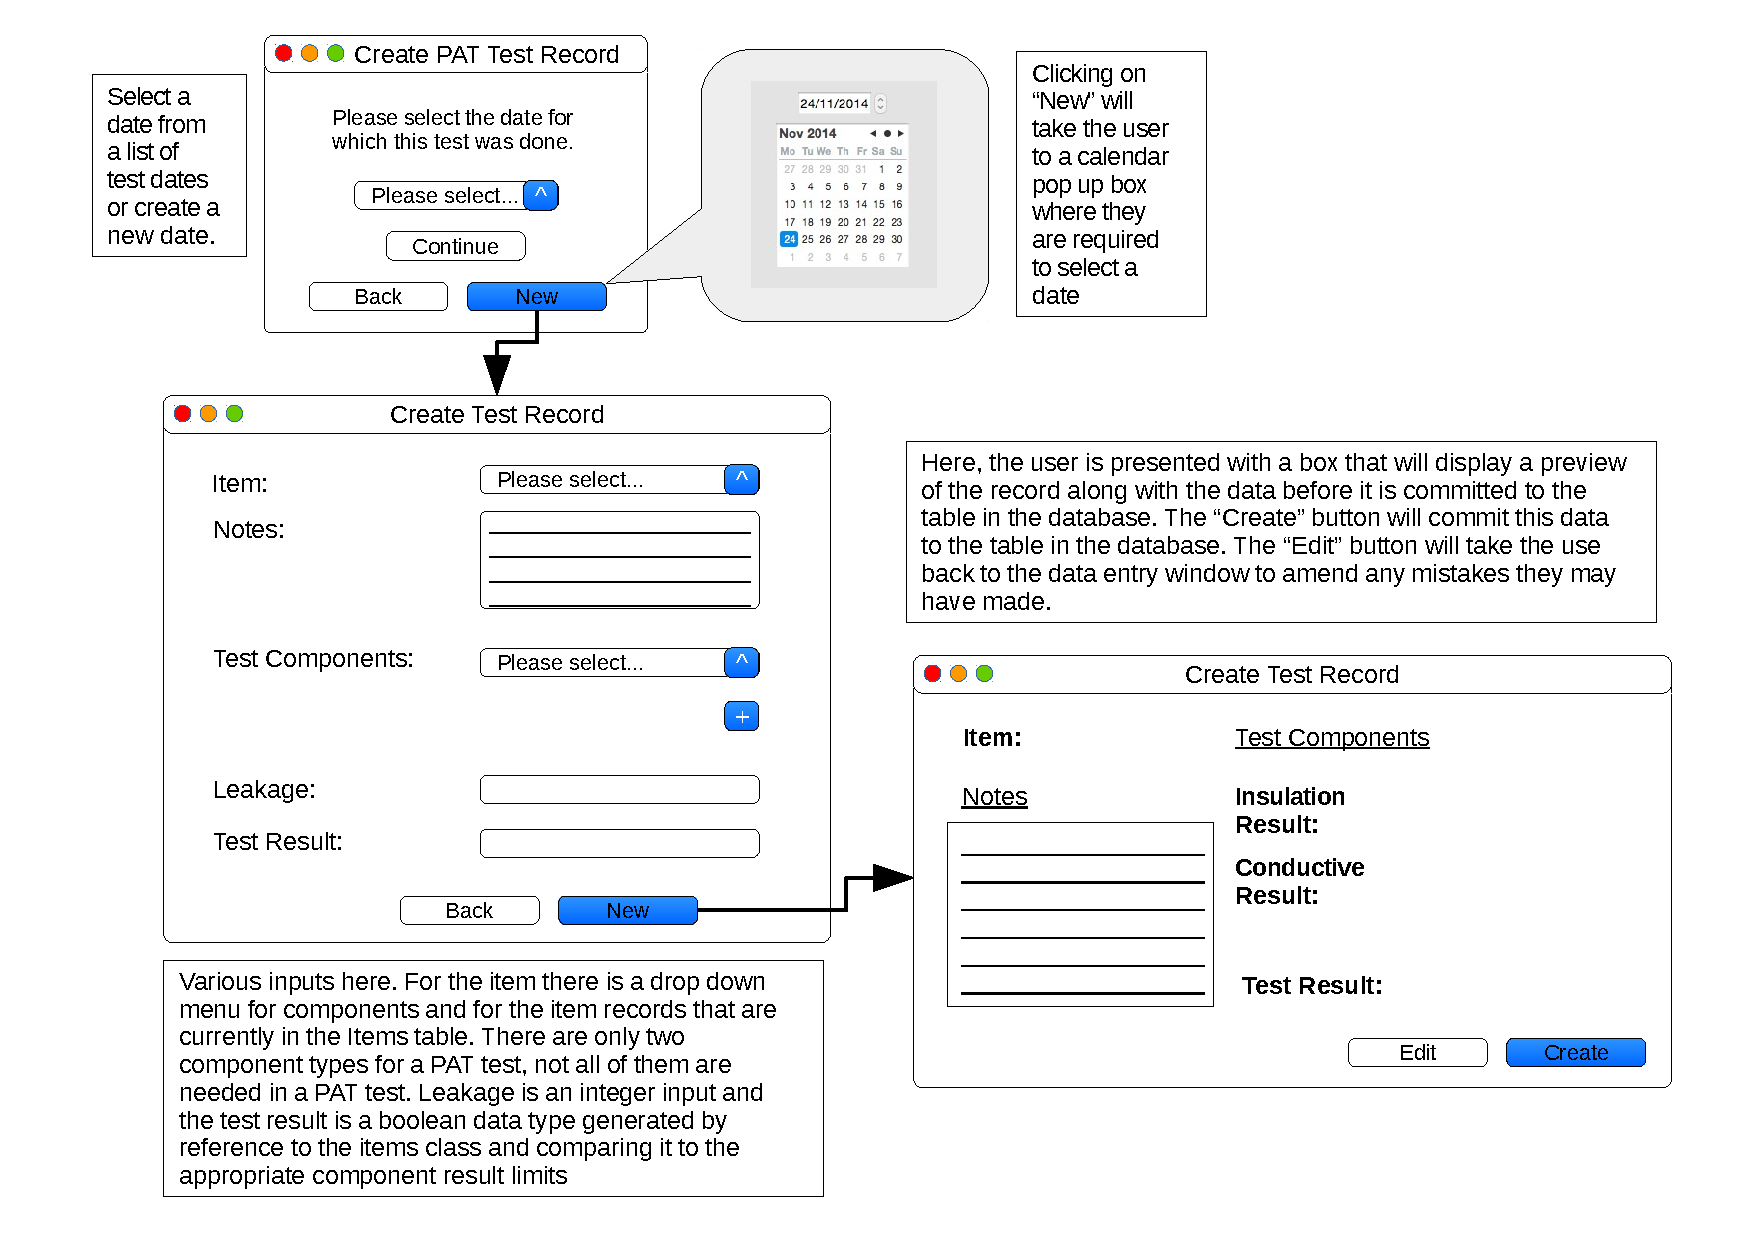
\includegraphics[width=500px]{./Design/user_interface/Add_pat_test_record_interface.pdf}
    \end{center}
    \caption{Login and Main Menu windows.} \label{fig:print_function_result}
\end{figure}

\end{landscape}

\section{Hardware Specification}

The hardware I am going to use are for a custom built Early 2008 Mac Pro. The specifications are as follows:
\begin{itemize}
    \item 2x 2.8 GHz Quad-Core Intel\textregistered Xeon\texttrademark Processor
    \item ATI Radeon HD 2600 XT 256MB Graphics Card
    \item 661-4449 Apple Mac Pro A1186 Motherboard
    \item 16.00GB DDR3 RAM
    \item 1TB SATA Disk-Drive
    \item 6TB RAID Storage
    \item Apple SuperDrive \\
\end{itemize}

I have chosen to build my system for this specification as this is the computer my client is going to run the application on, it is also a low cost choice of system spec to run on as the hardware has already been bought and is therefore ready and available to use.

\begin{landscape}

=======
\section{Hardware Specification}

>>>>>>> FETCH_HEAD
\section{Program Structure}

\subsection{Top-down design structure charts}

\begin{figure}[H]
    \begin{center}
    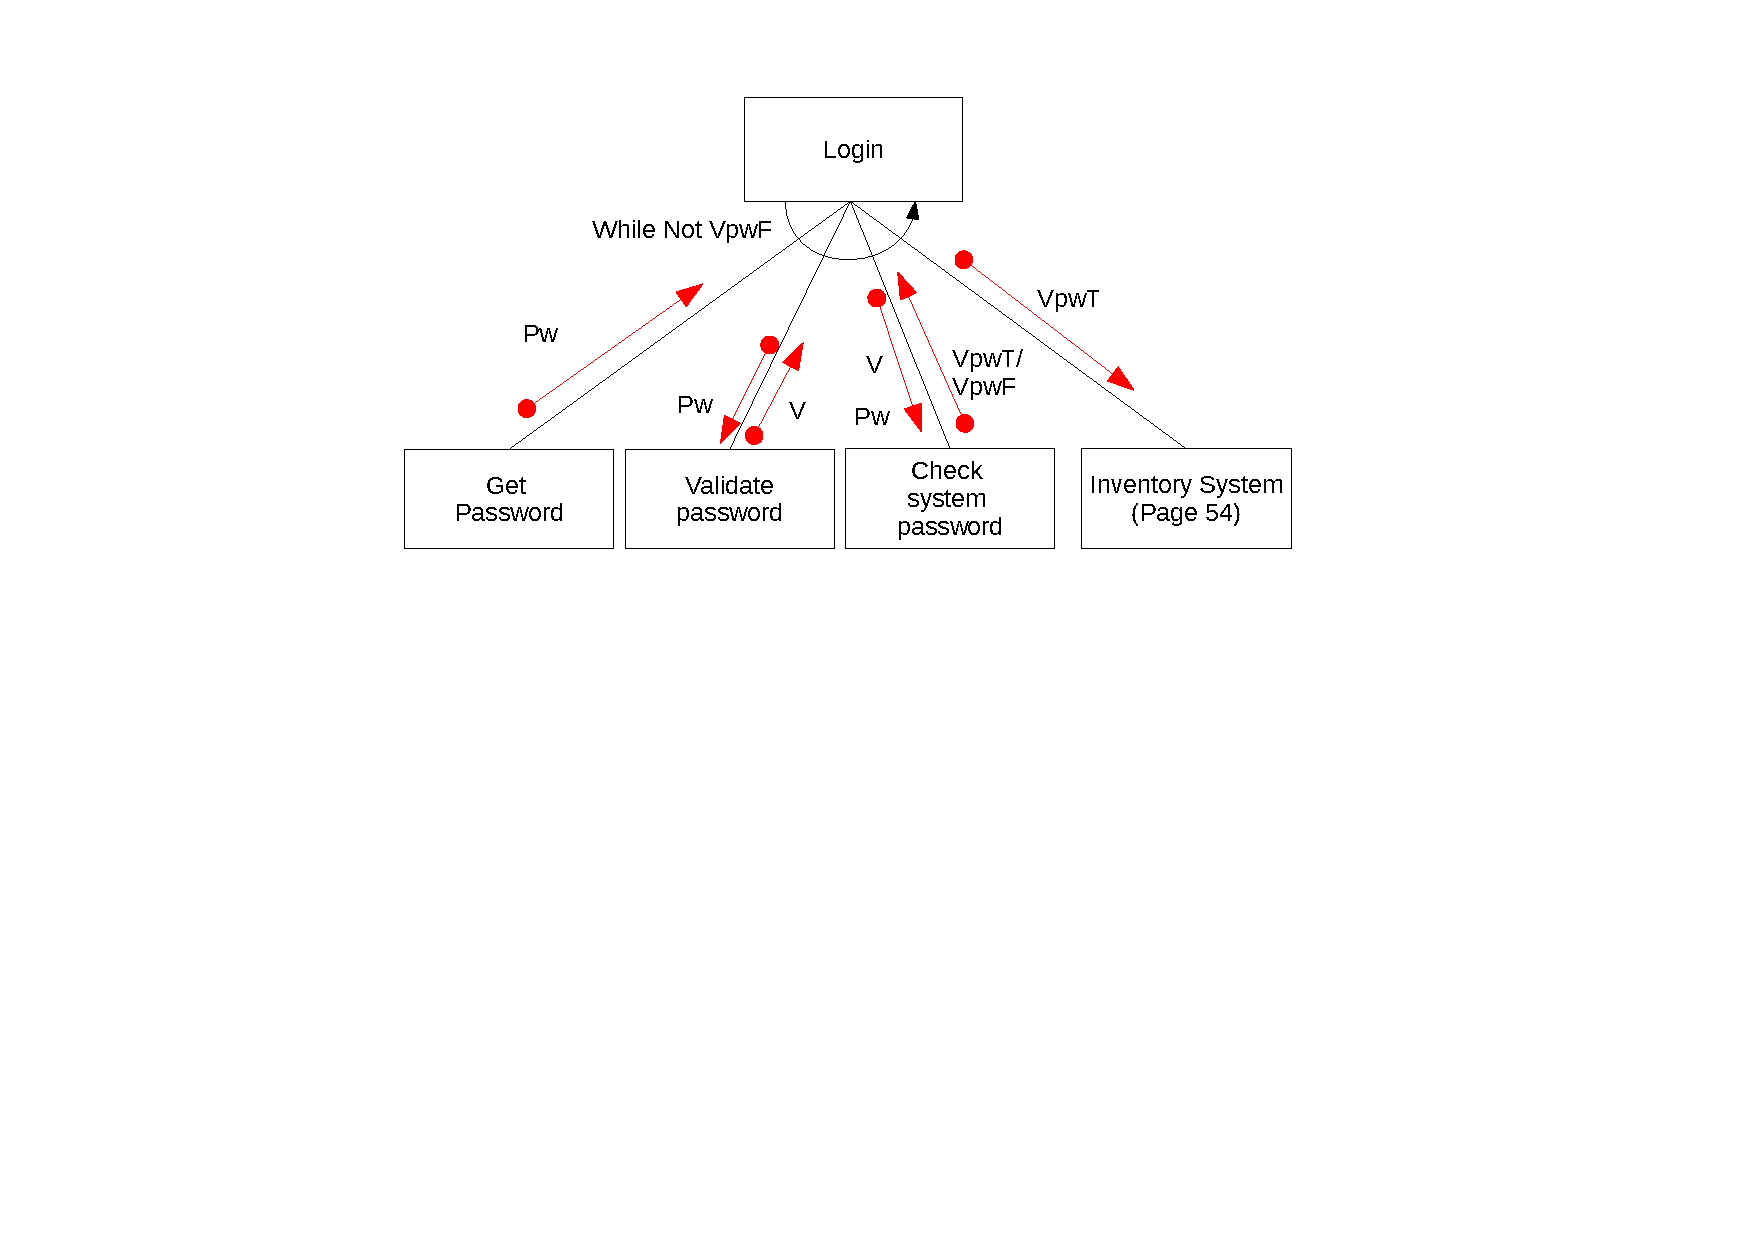
\includegraphics[width=500px]{./Design/top_down_design/Top_down_design.pdf}
    \caption{Object Diagram.} \label{fig:object_diagram}
    \end{center}
\end{figure}

\newpage

\begin{figure}[H]
    \begin{center}
    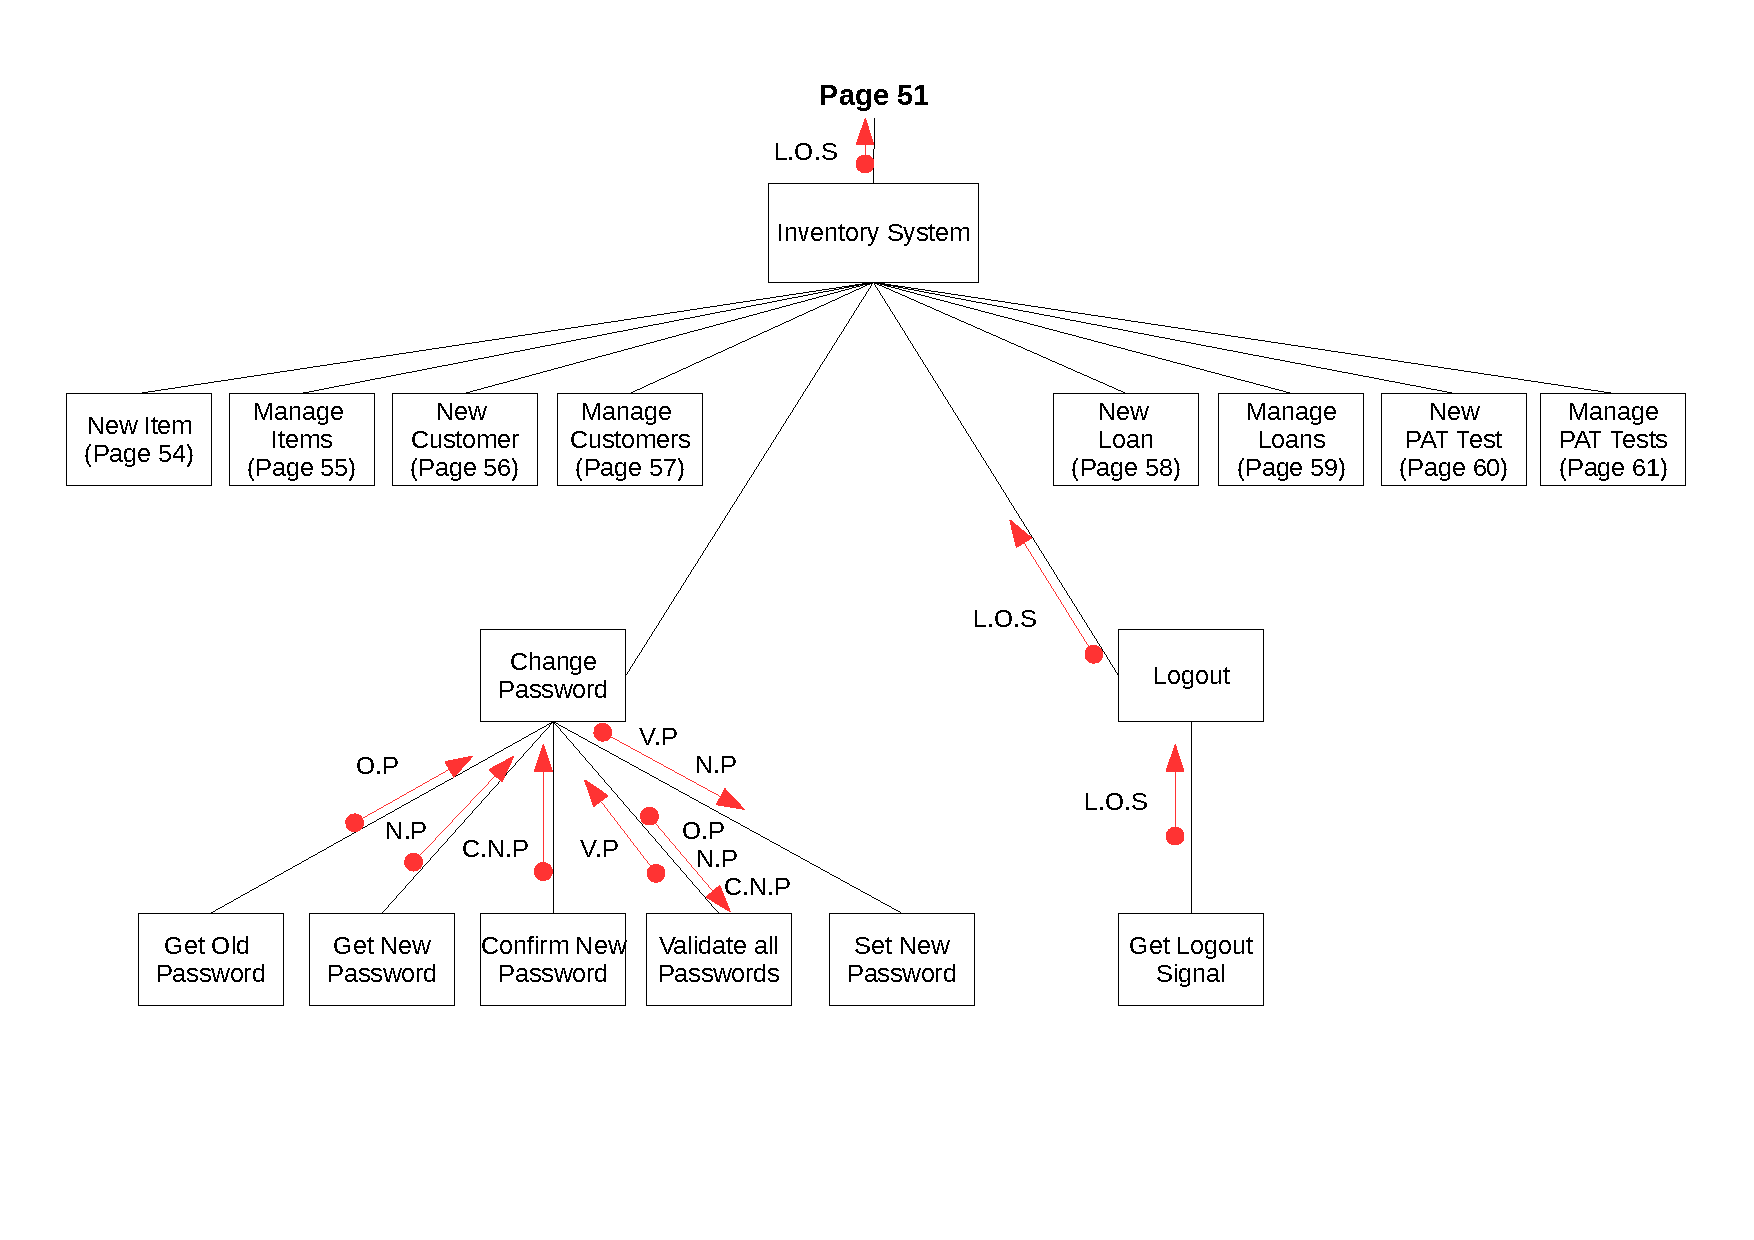
\includegraphics[width=500px]{./Design/top_down_design/inventory_system.pdf}
    \caption{Object Diagram.} \label{fig:object_diagram}
    \end{center}
\end{figure}

\newpage

\begin{figure}[H]
    \begin{center}
    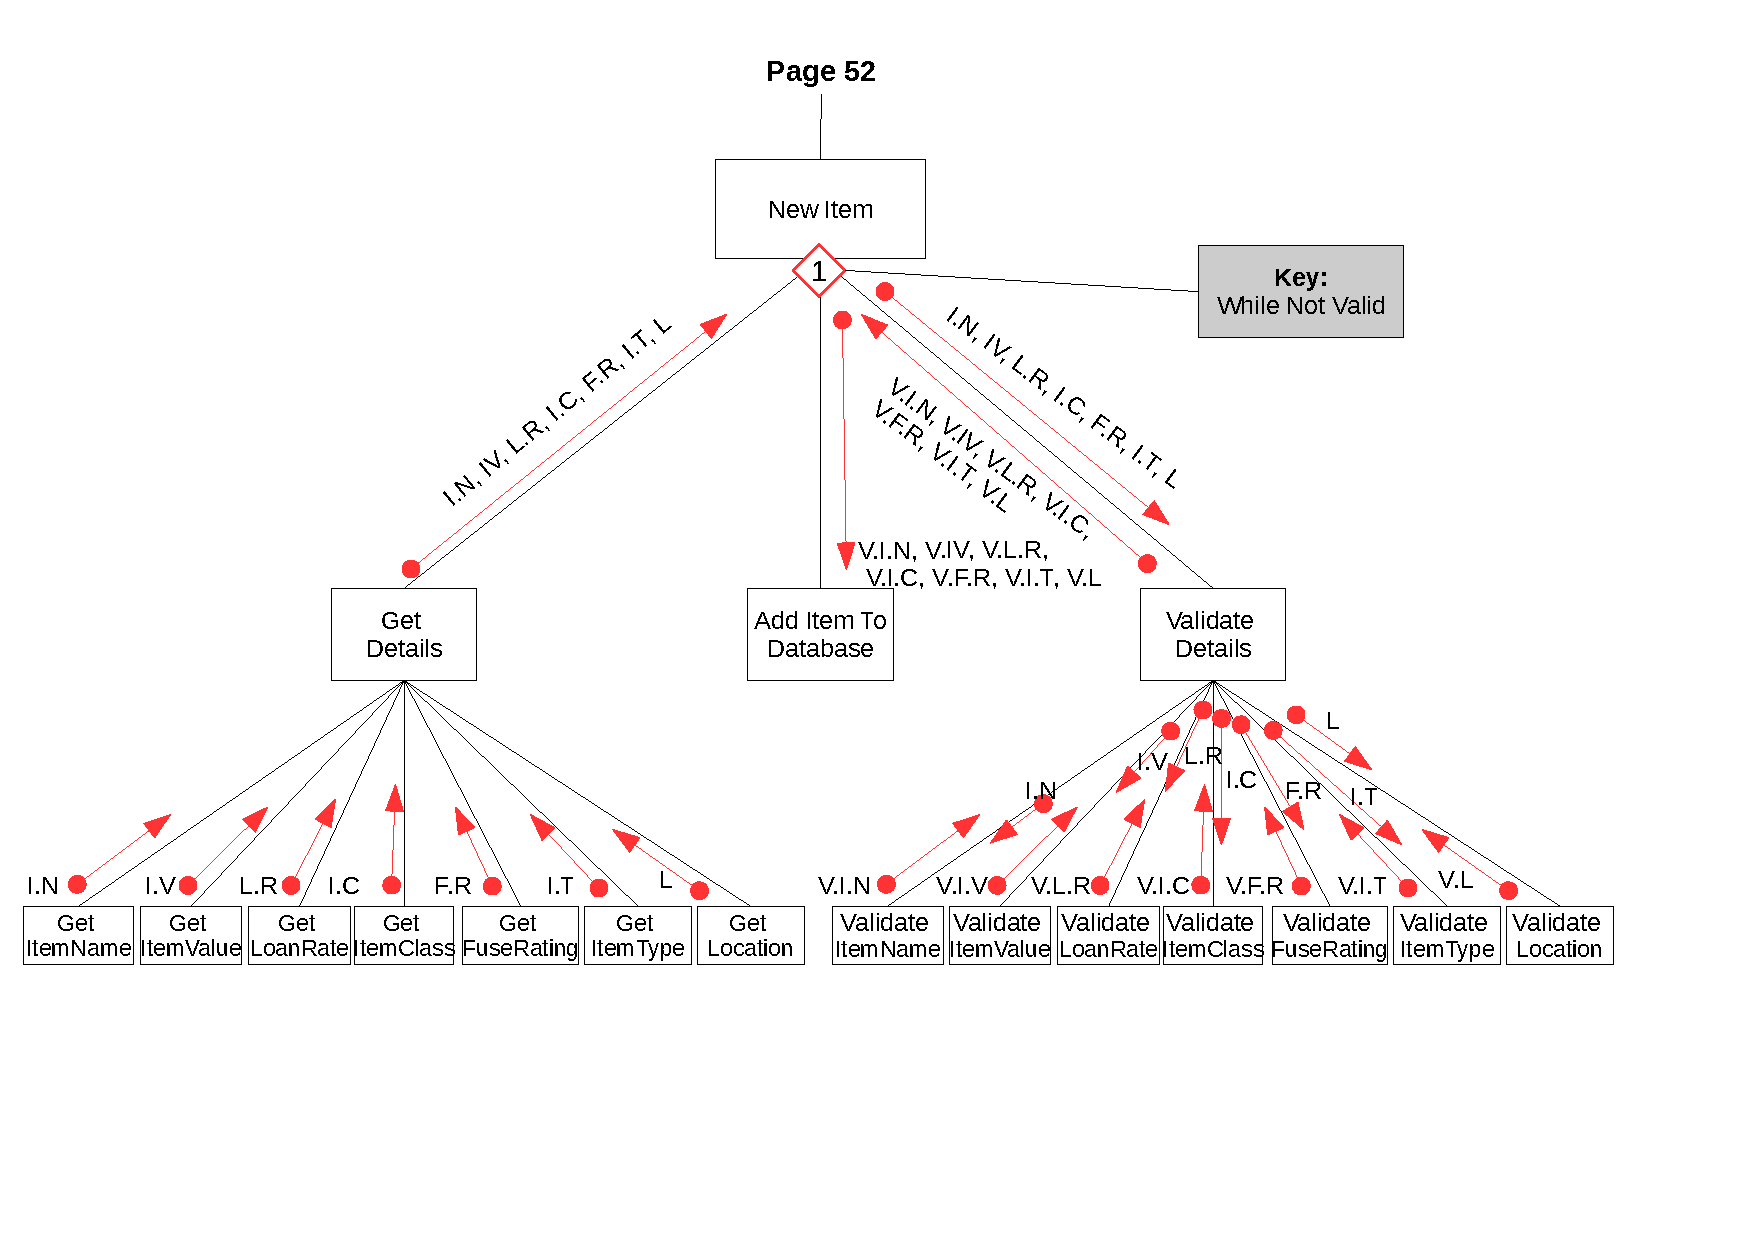
\includegraphics[width=500px]{./Design/top_down_design/new_item.pdf}
    \caption{Object Diagram.} \label{fig:object_diagram}
    \end{center}
\end{figure}

\newpage

\begin{figure}[H]
    \begin{center}
    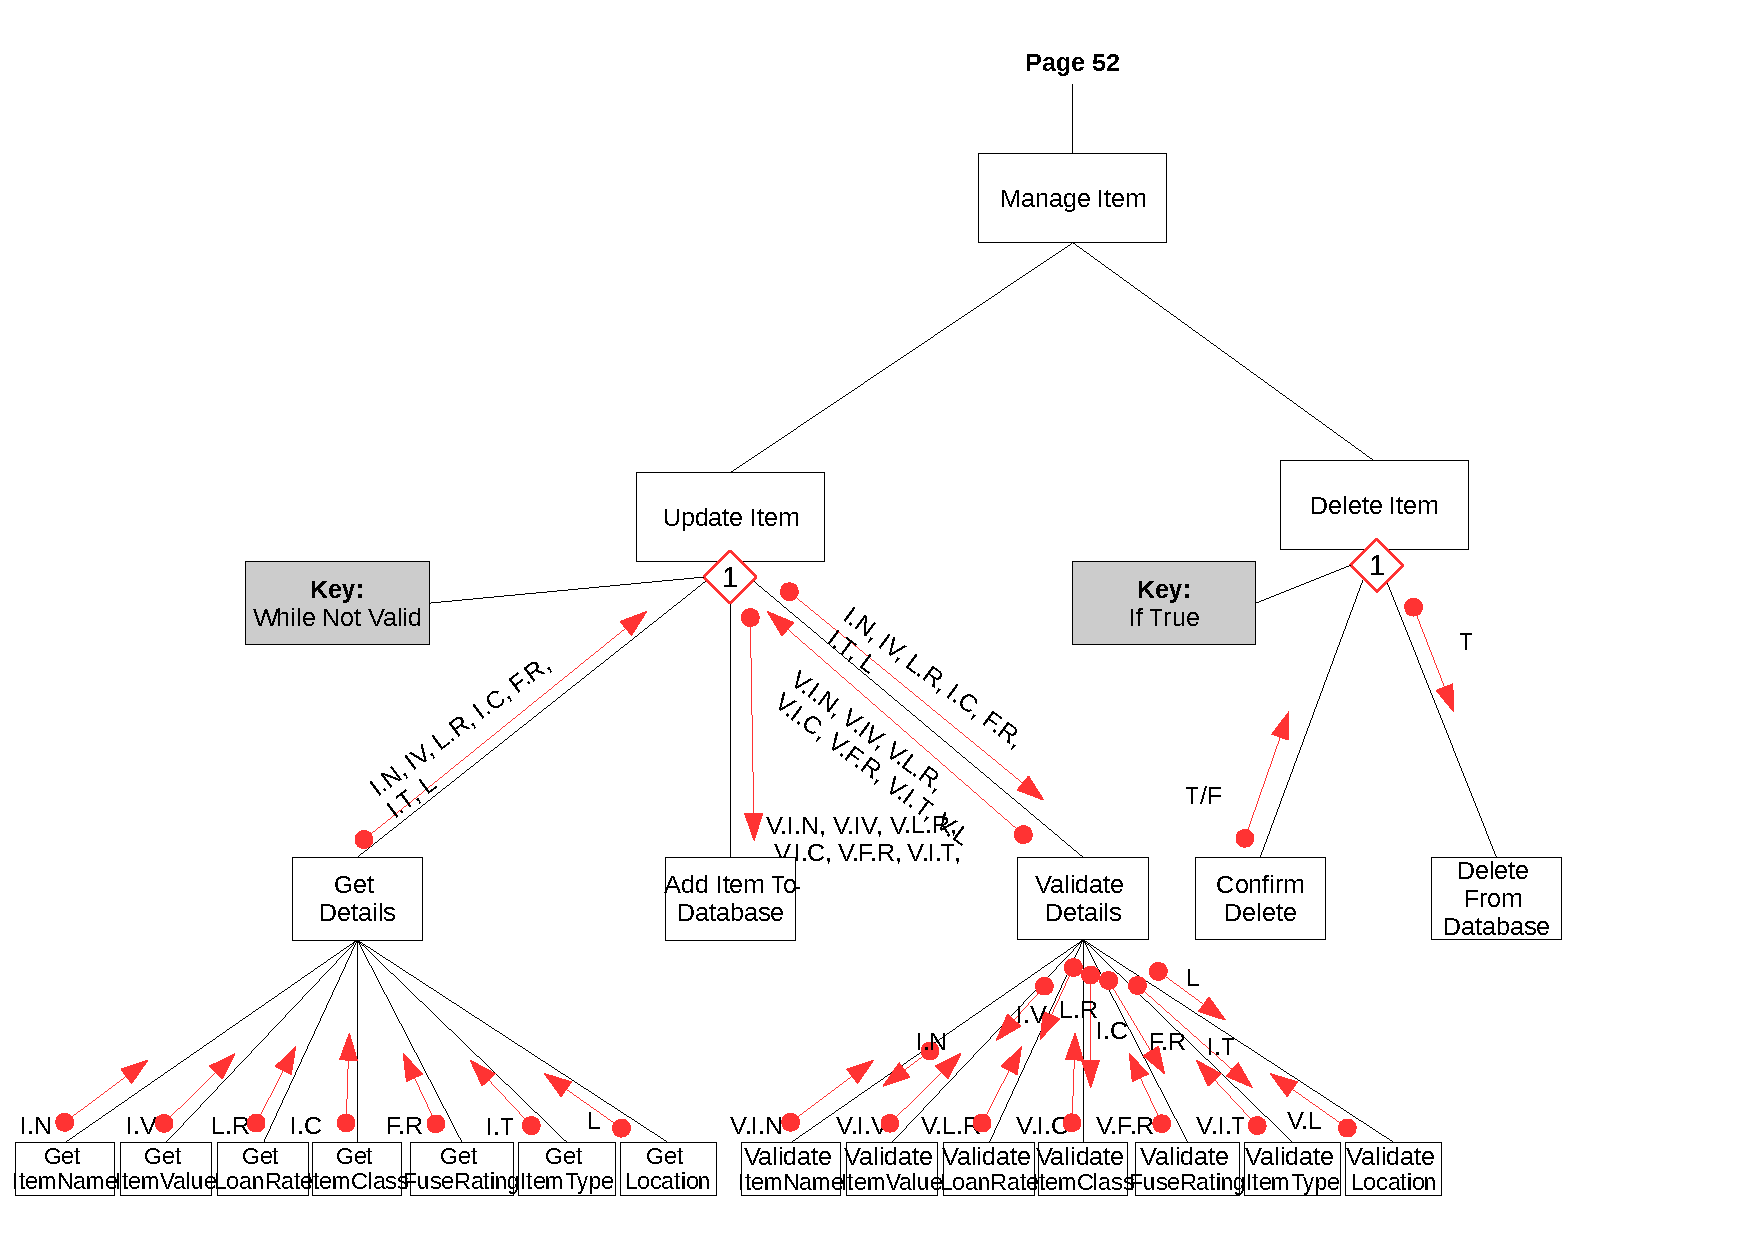
\includegraphics[width=500px]{./Design/top_down_design/manage_items.pdf}
    \caption{Object Diagram.} \label{fig:object_diagram}
    \end{center}
\end{figure}

\newpage

\begin{figure}[H]
    \begin{center}
    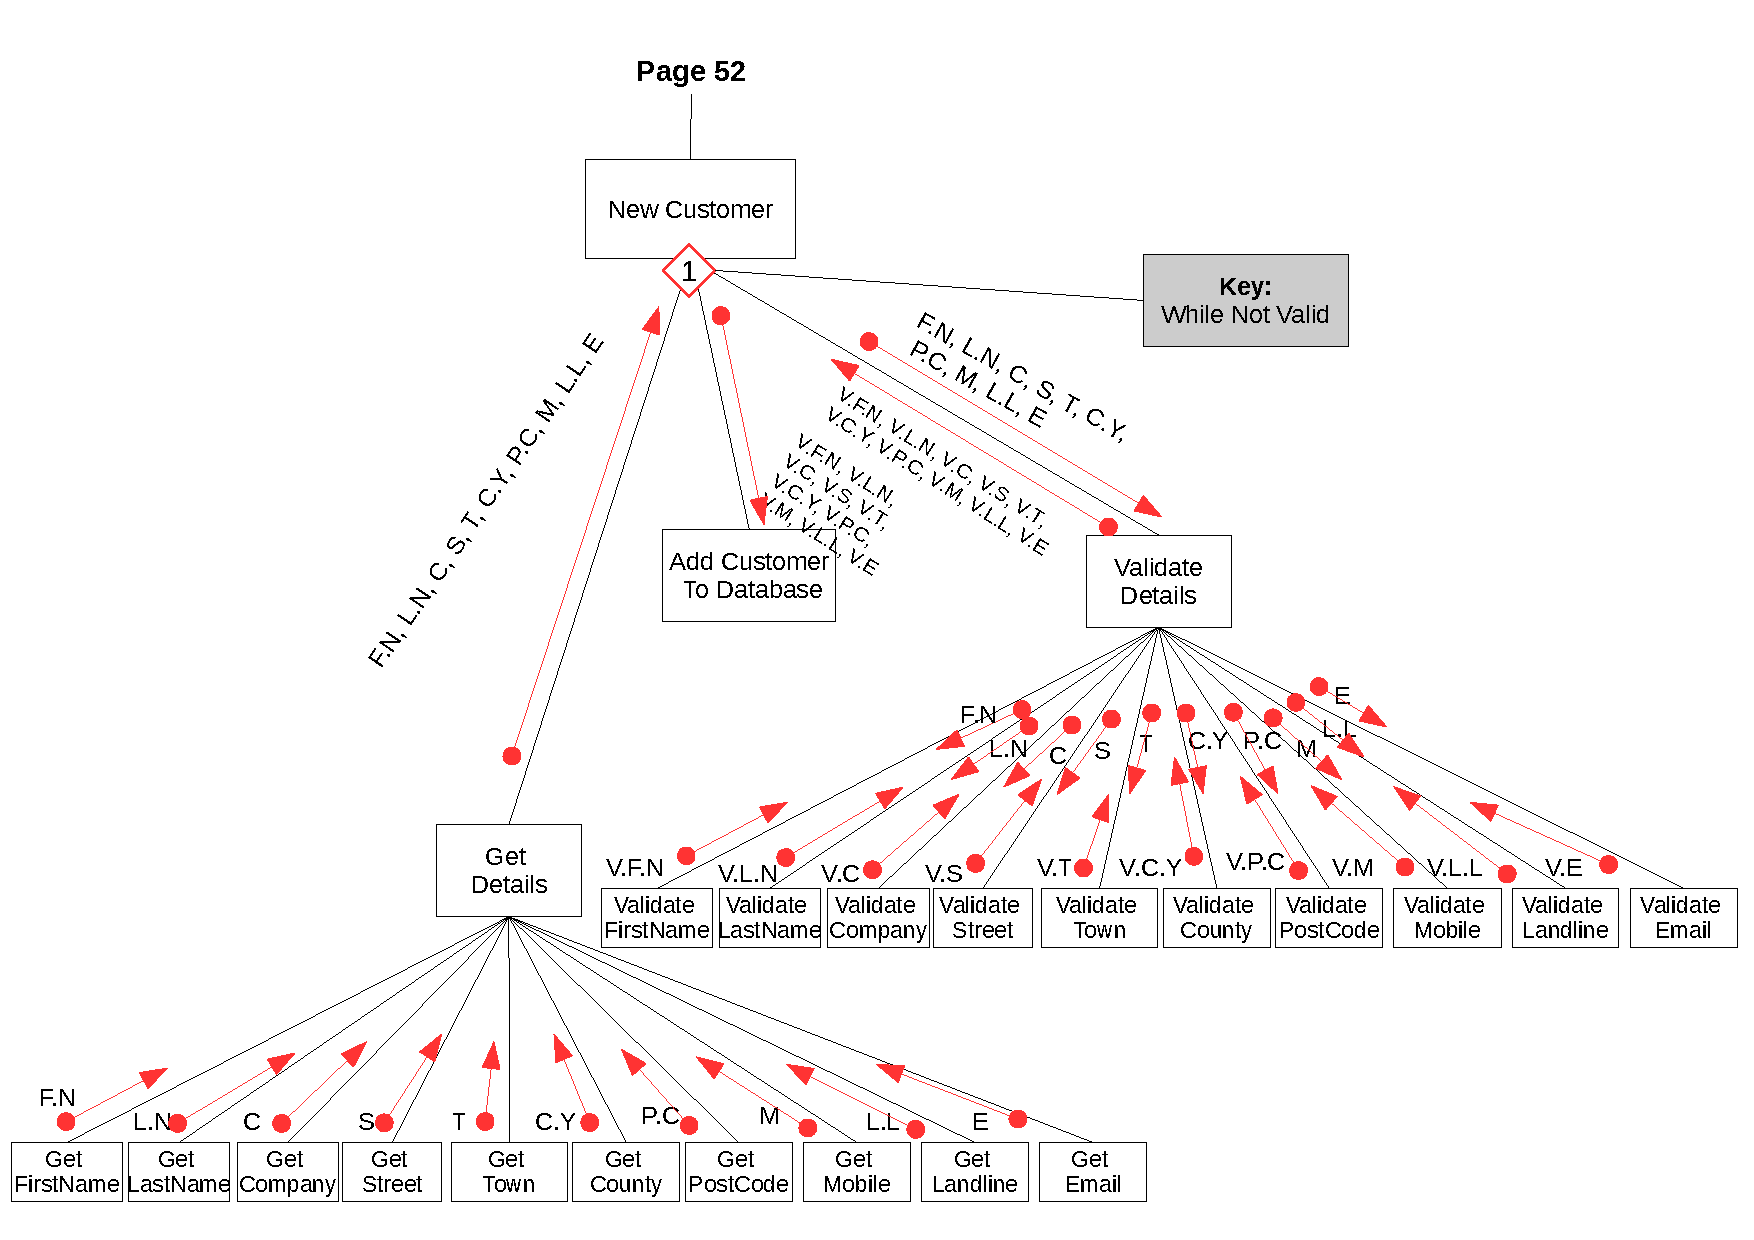
\includegraphics[width=500px]{./Design/top_down_design/new_customer.pdf}
    \caption{Object Diagram.} \label{fig:object_diagram}
    \end{center}
\end{figure}

\newpage

\begin{figure}[H]
    \begin{center}
    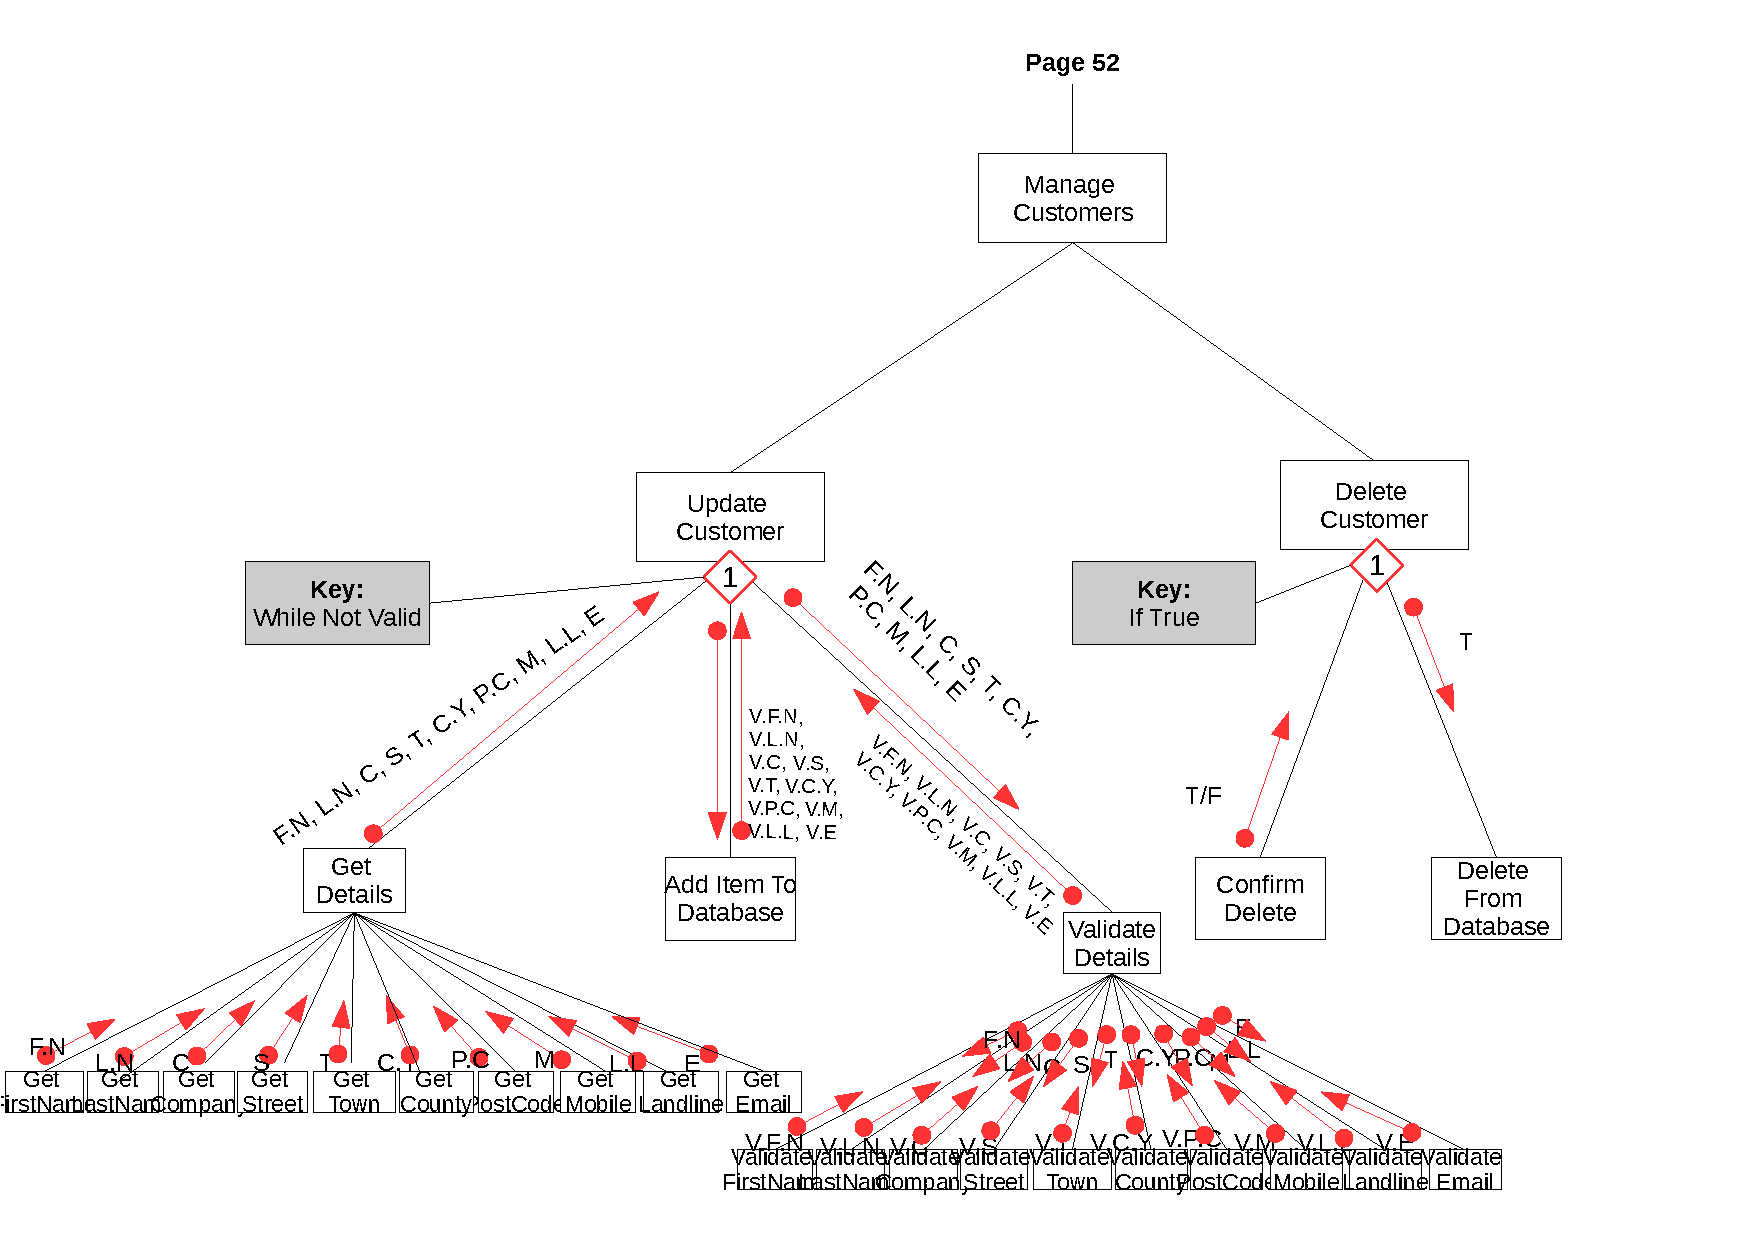
\includegraphics[width=500px]{./Design/top_down_design/manage_customers.pdf}
    \caption{Object Diagram.} \label{fig:object_diagram}
    \end{center}
\end{figure}

\newpage

\begin{figure}[H]
    \begin{center}
    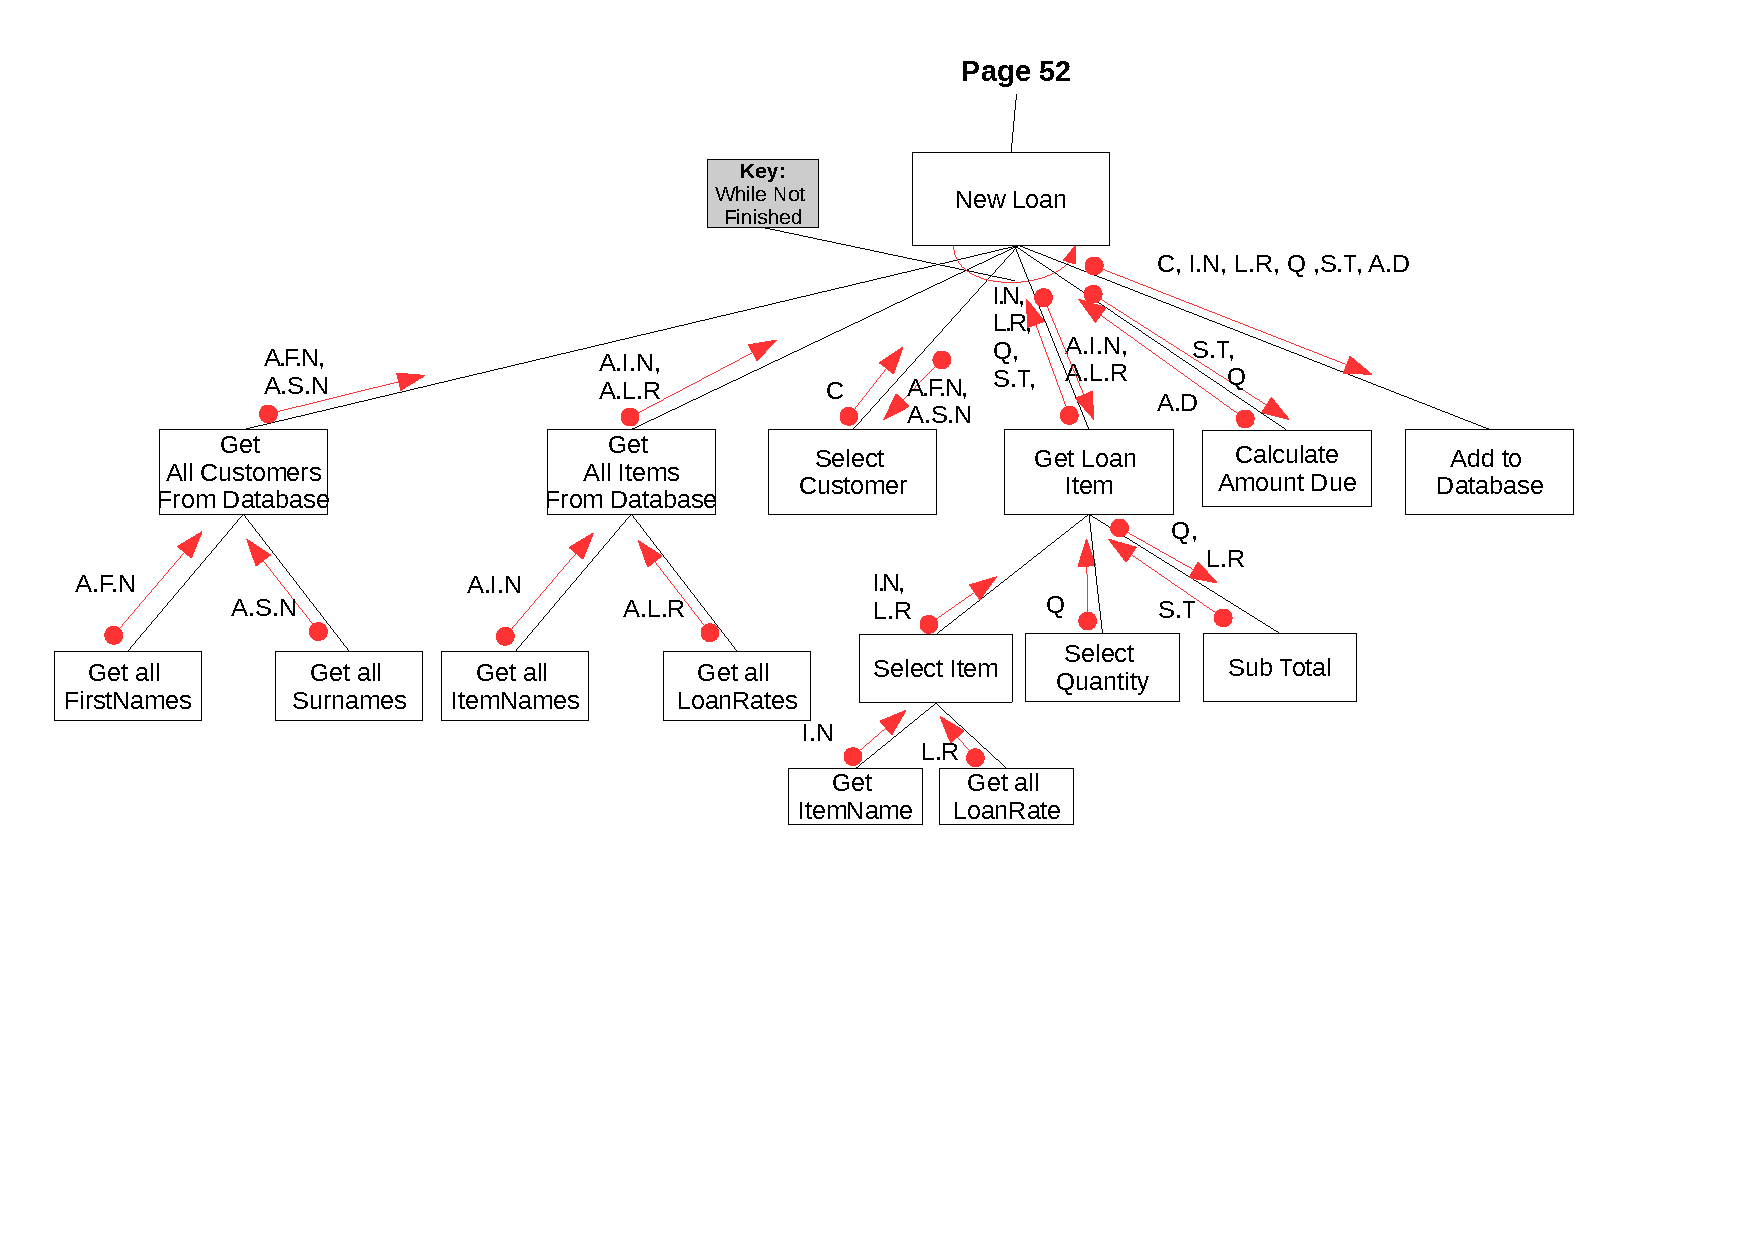
\includegraphics[width=500px]{./Design/top_down_design/new_loan.pdf}
    \caption{Object Diagram.} \label{fig:object_diagram}
    \end{center}
\end{figure}

\newpage

\begin{figure}[H]
    \begin{center}
    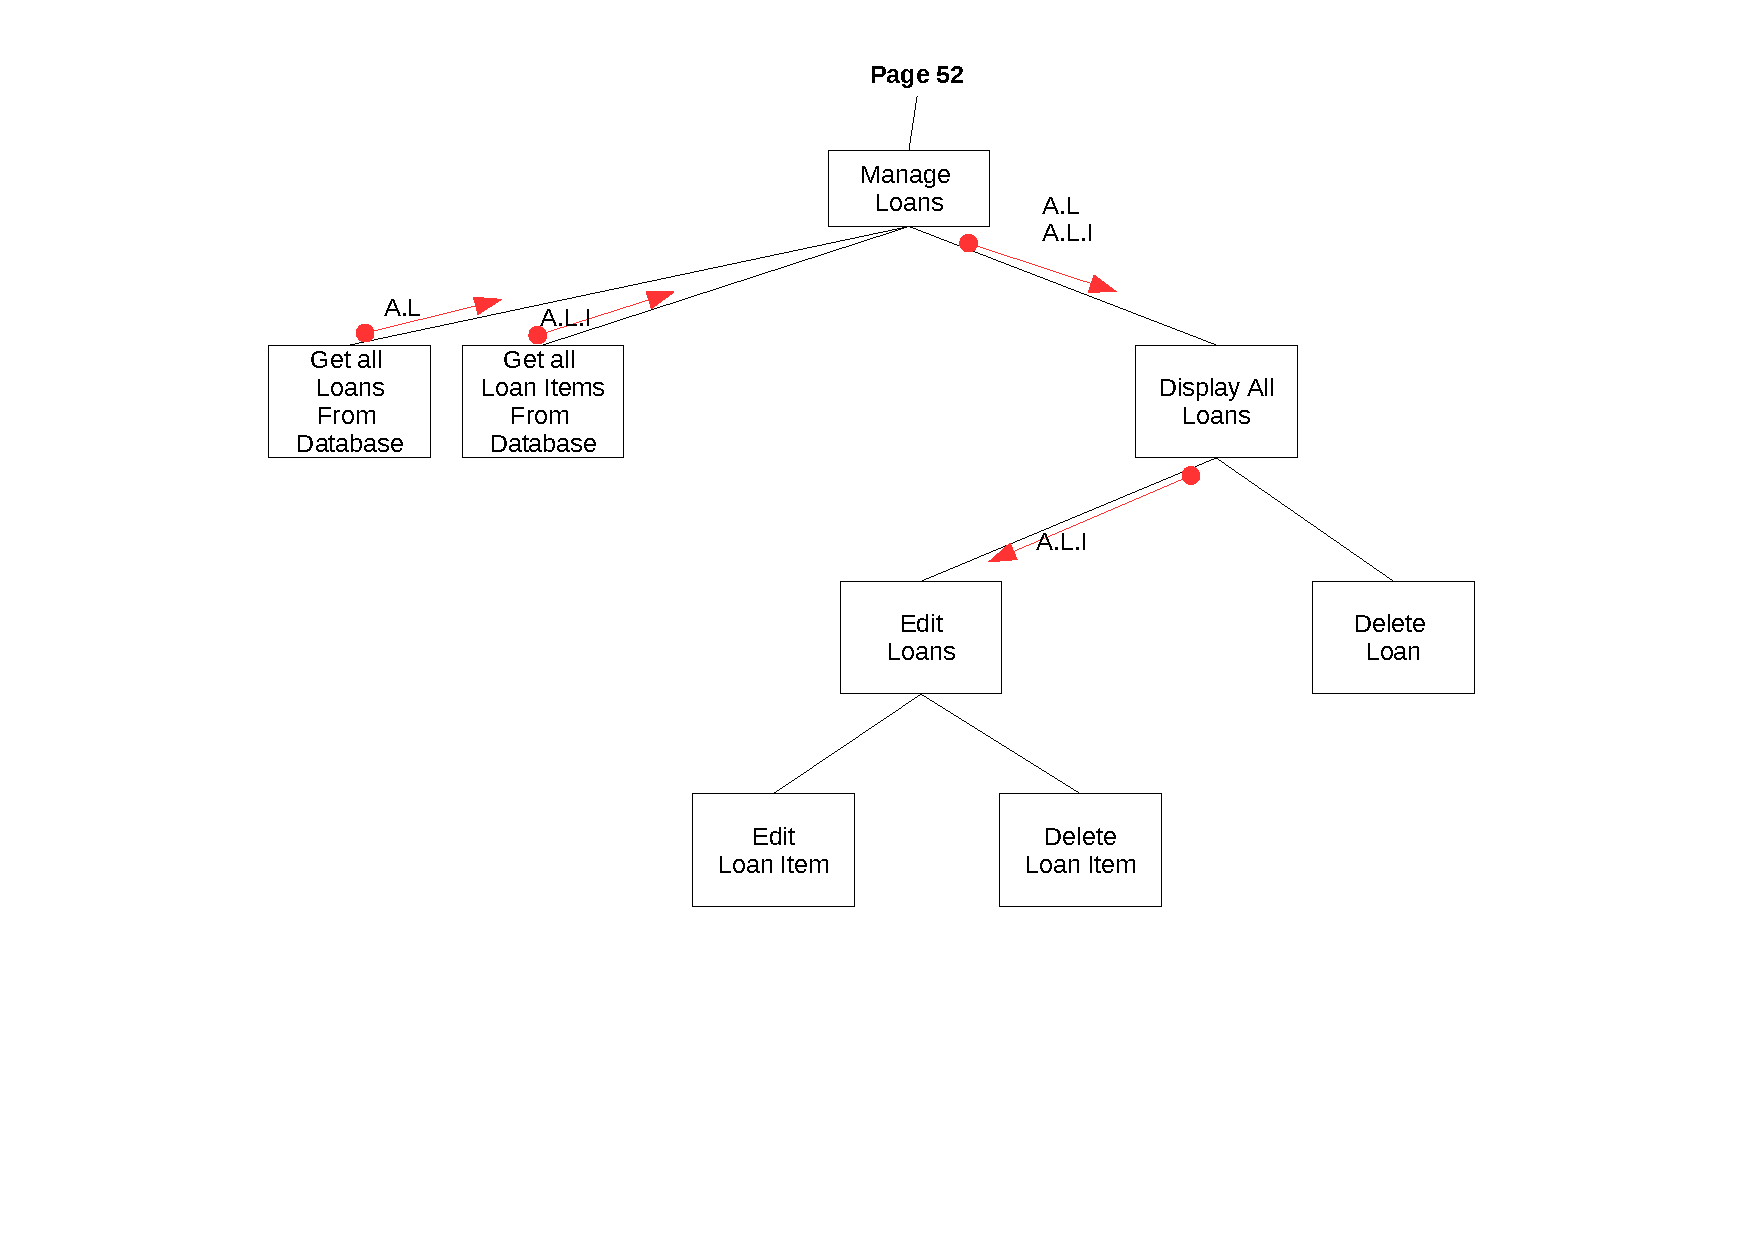
\includegraphics[width=500px]{./Design/top_down_design/manage_loans.pdf}
    \caption{Object Diagram.} \label{fig:object_diagram}
    \end{center}
\end{figure}

\newpage

\begin{figure}[H]
    \begin{center}
    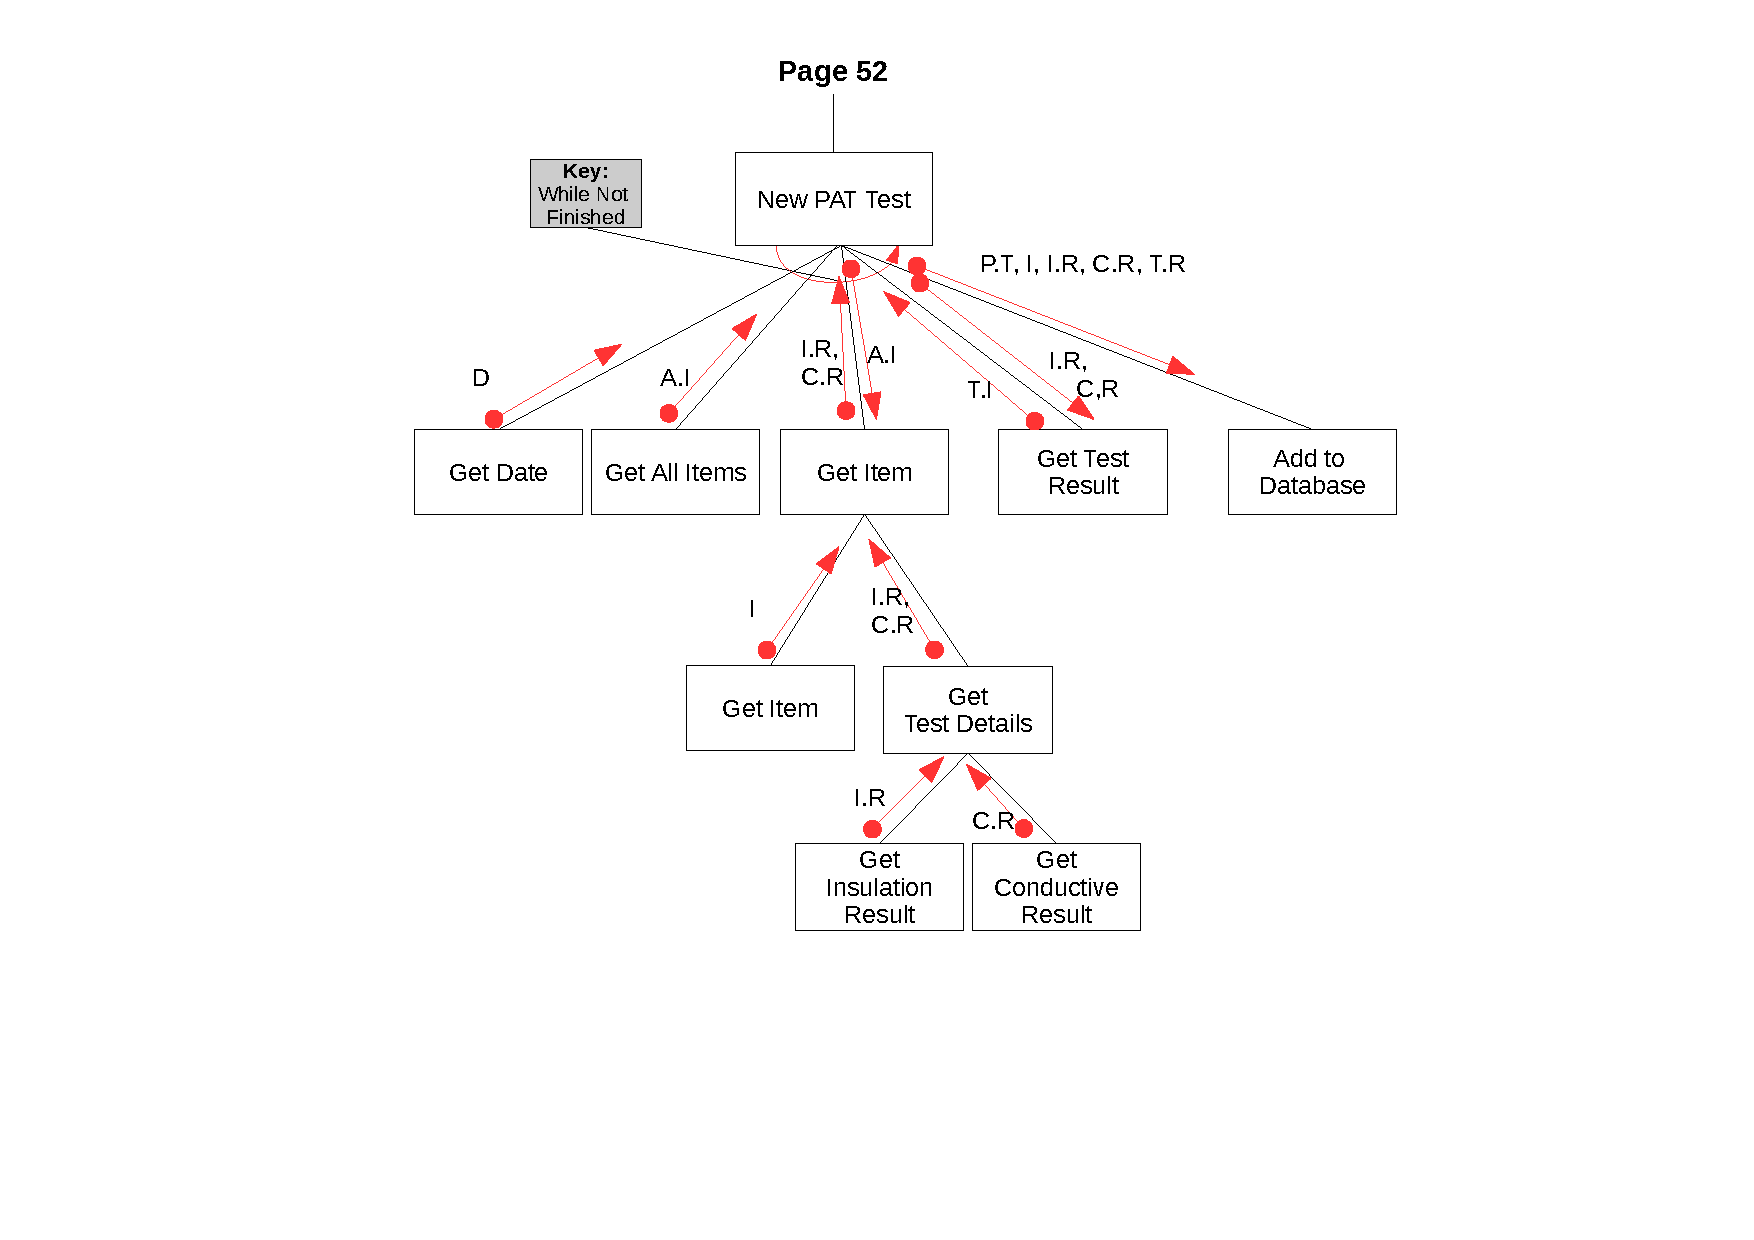
\includegraphics[width=500px]{./Design/top_down_design/new_pat_test}
    \caption{Object Diagram.} \label{fig:object_diagram}
    \end{center}
\end{figure}

\newpage

\begin{figure}[H]
    \begin{center}
    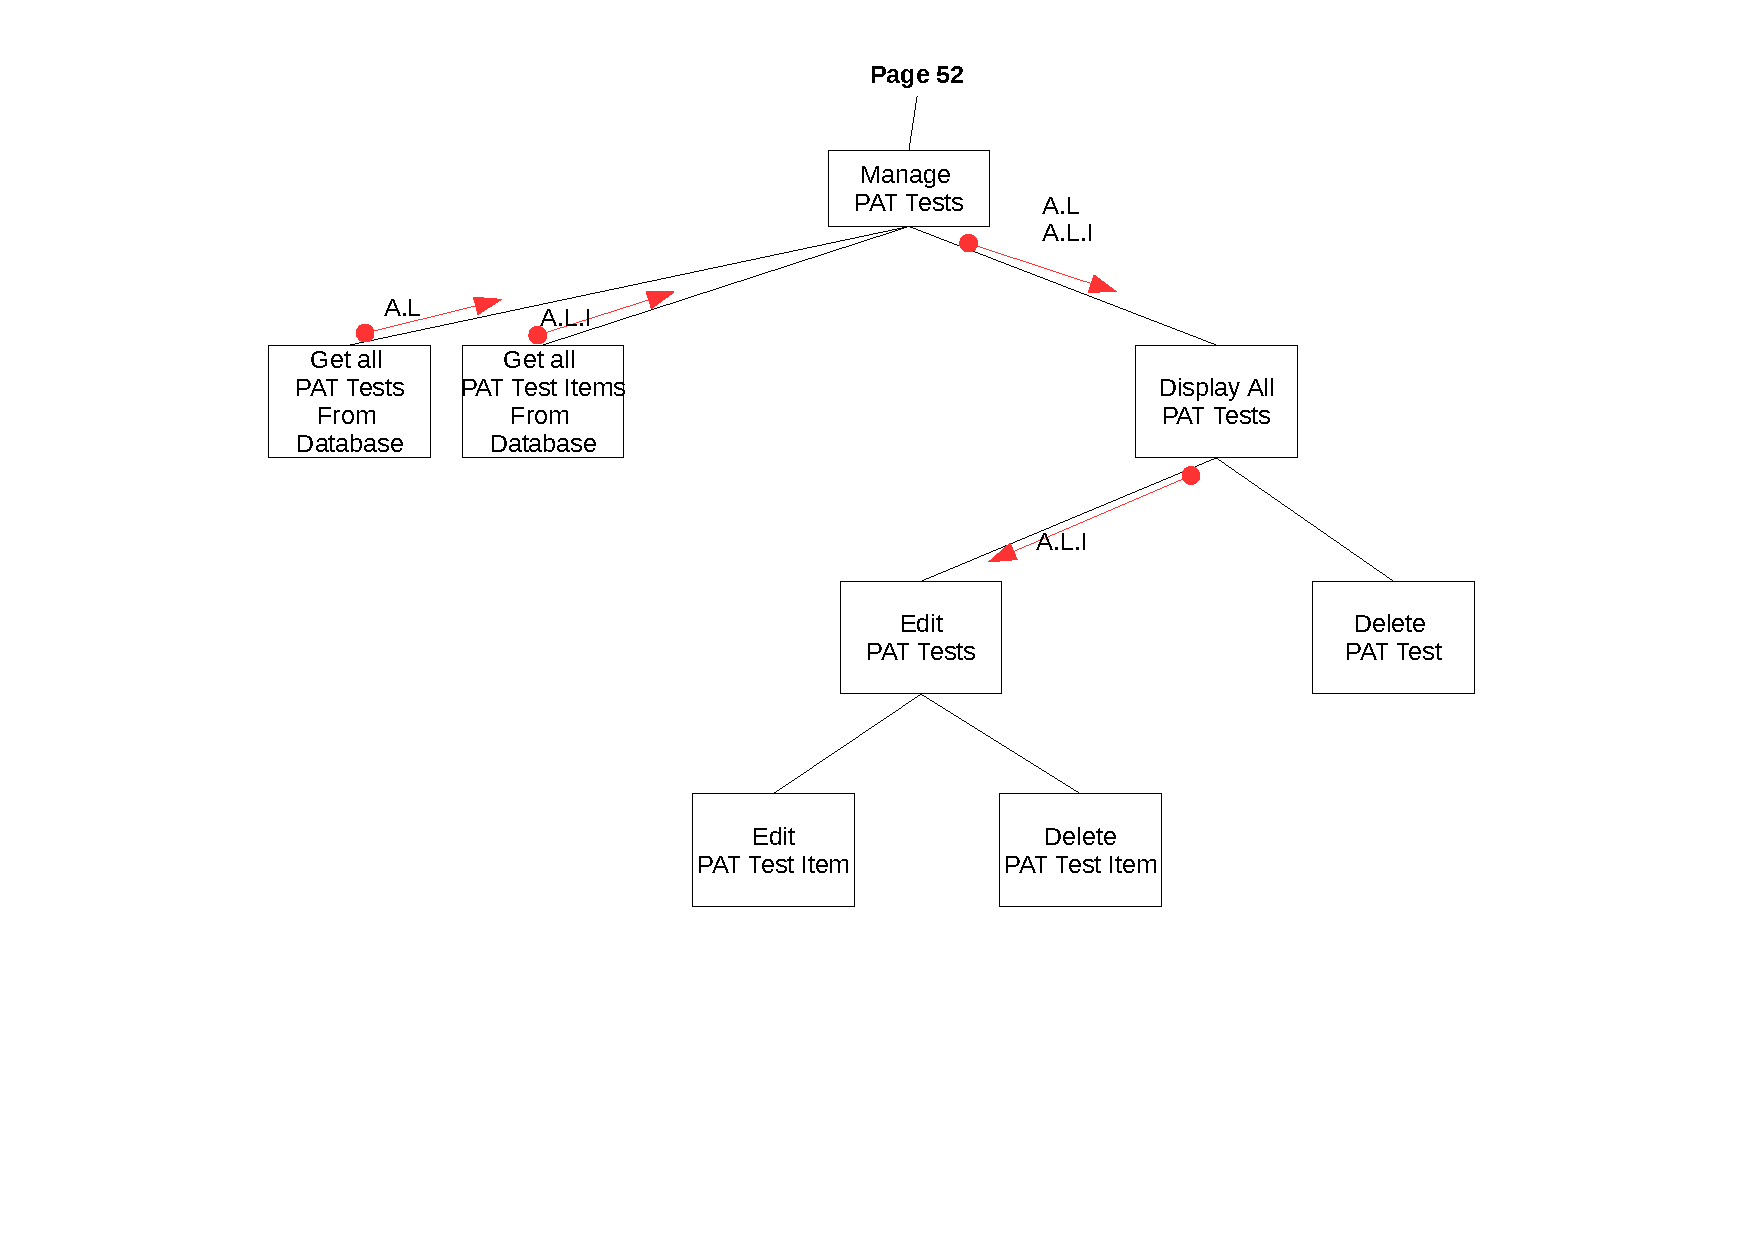
\includegraphics[width=500px]{./Design/top_down_design/manage_pat_tests.pdf}
    \caption{Object Diagram.} \label{fig:object_diagram}
    \end{center}
\end{figure}


\end{landscape}


\subsection{Algorithms in pseudo-code for each data transformation process}

\begin{algorithm}[H]
    \caption{Producing a PDF via print function}
\begin{algorithmic}[1]
\SET{$officeAddr$}{$['Street','Town','County','PostCode']$}
\SET{$loanItems$}{$self.getItemsInLoan()$}
\SET{$customerDets$}{$self.getCustomerDetails$}

\For{$item$}{$loanItems$}
    \SET{$loanRate$}{$item[2]$}
    \SET{$amountDue$}{$amountDue + loanRate$}
\EndFor
\SET{$amountIncVAT$}{$amountDue * 1.2$}

\SET{$invoiceInfo$}{$[officeAddr, loanItems, customerDets, amountDue, amountIncVAT]$}
\SET{$htmlInvoice$}{$self.createHtmlInvoice(invoiceInfo)$}

\SET{$self.printer$}{$QPrinter()$}
\SET{$printerDialog$}{$QPrintDialog(self.printer, self)$}

\If{$printerDialog.exec_()$}
    \SET{$document$}{$QTextDocument$}
    \SET{$document.setHtml$}{$html$}
    \SET{$document.Print$}{$self.printer$}
    \State
    \SET{$message$}{$"The document printed successfully"$}
    \SET{$QMessageBox.information$}{$self, "Print Successful", message $}
\Else
    \SET{$message$}{$"The document was unable to print."$}
    \SET{$QMessageBox.information$}{$self, "Print Failed", message $}
\EndIf
\end{algorithmic}
\end{algorithm}

\begin{center}
    NB. The reason that "document.Print" has a capitalised 'P' is because\\
    LaTeX doesn't like the underscore that should be after it
\end{center}

\begin{landscape}

\subsection{Object Diagrams}

\begin{figure}[H]
    \begin{center}
    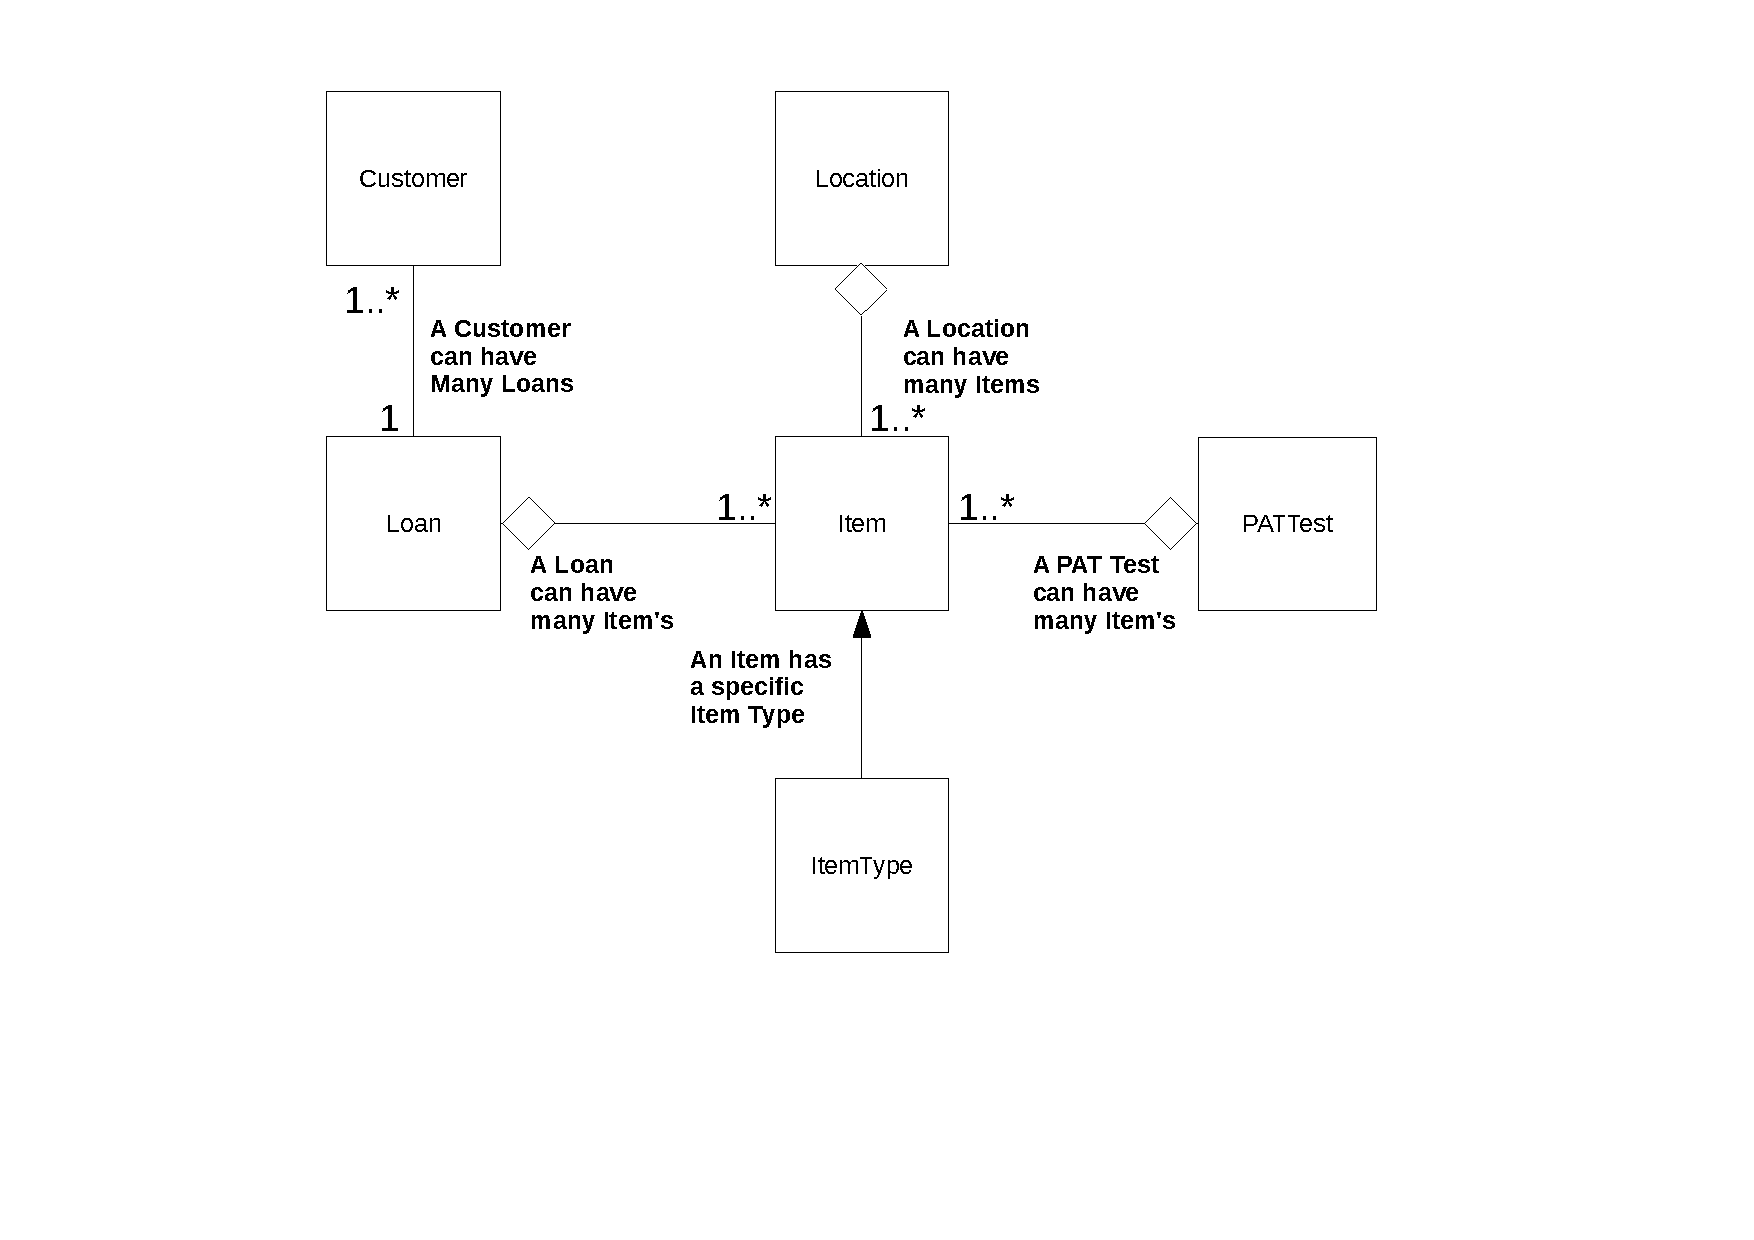
\includegraphics[height=325px]{./Design/Object_Diagrams/Object_diagrams.pdf}
    \caption{Object Diagram.} \label{fig:object_diagram}
    \end{center}
\end{figure}

\newpage

\subsection{Class Definitions}

\begin{figure}[H]
    \centerline{\includegraphics[width=50px]{./Design/Class_Definitions/Class_definition_key.pdf}}
    \caption{Class Diagram Key.} \label{fig:relationship_diagram}
\end{figure}

\begin{figure}[H]
    \centerline{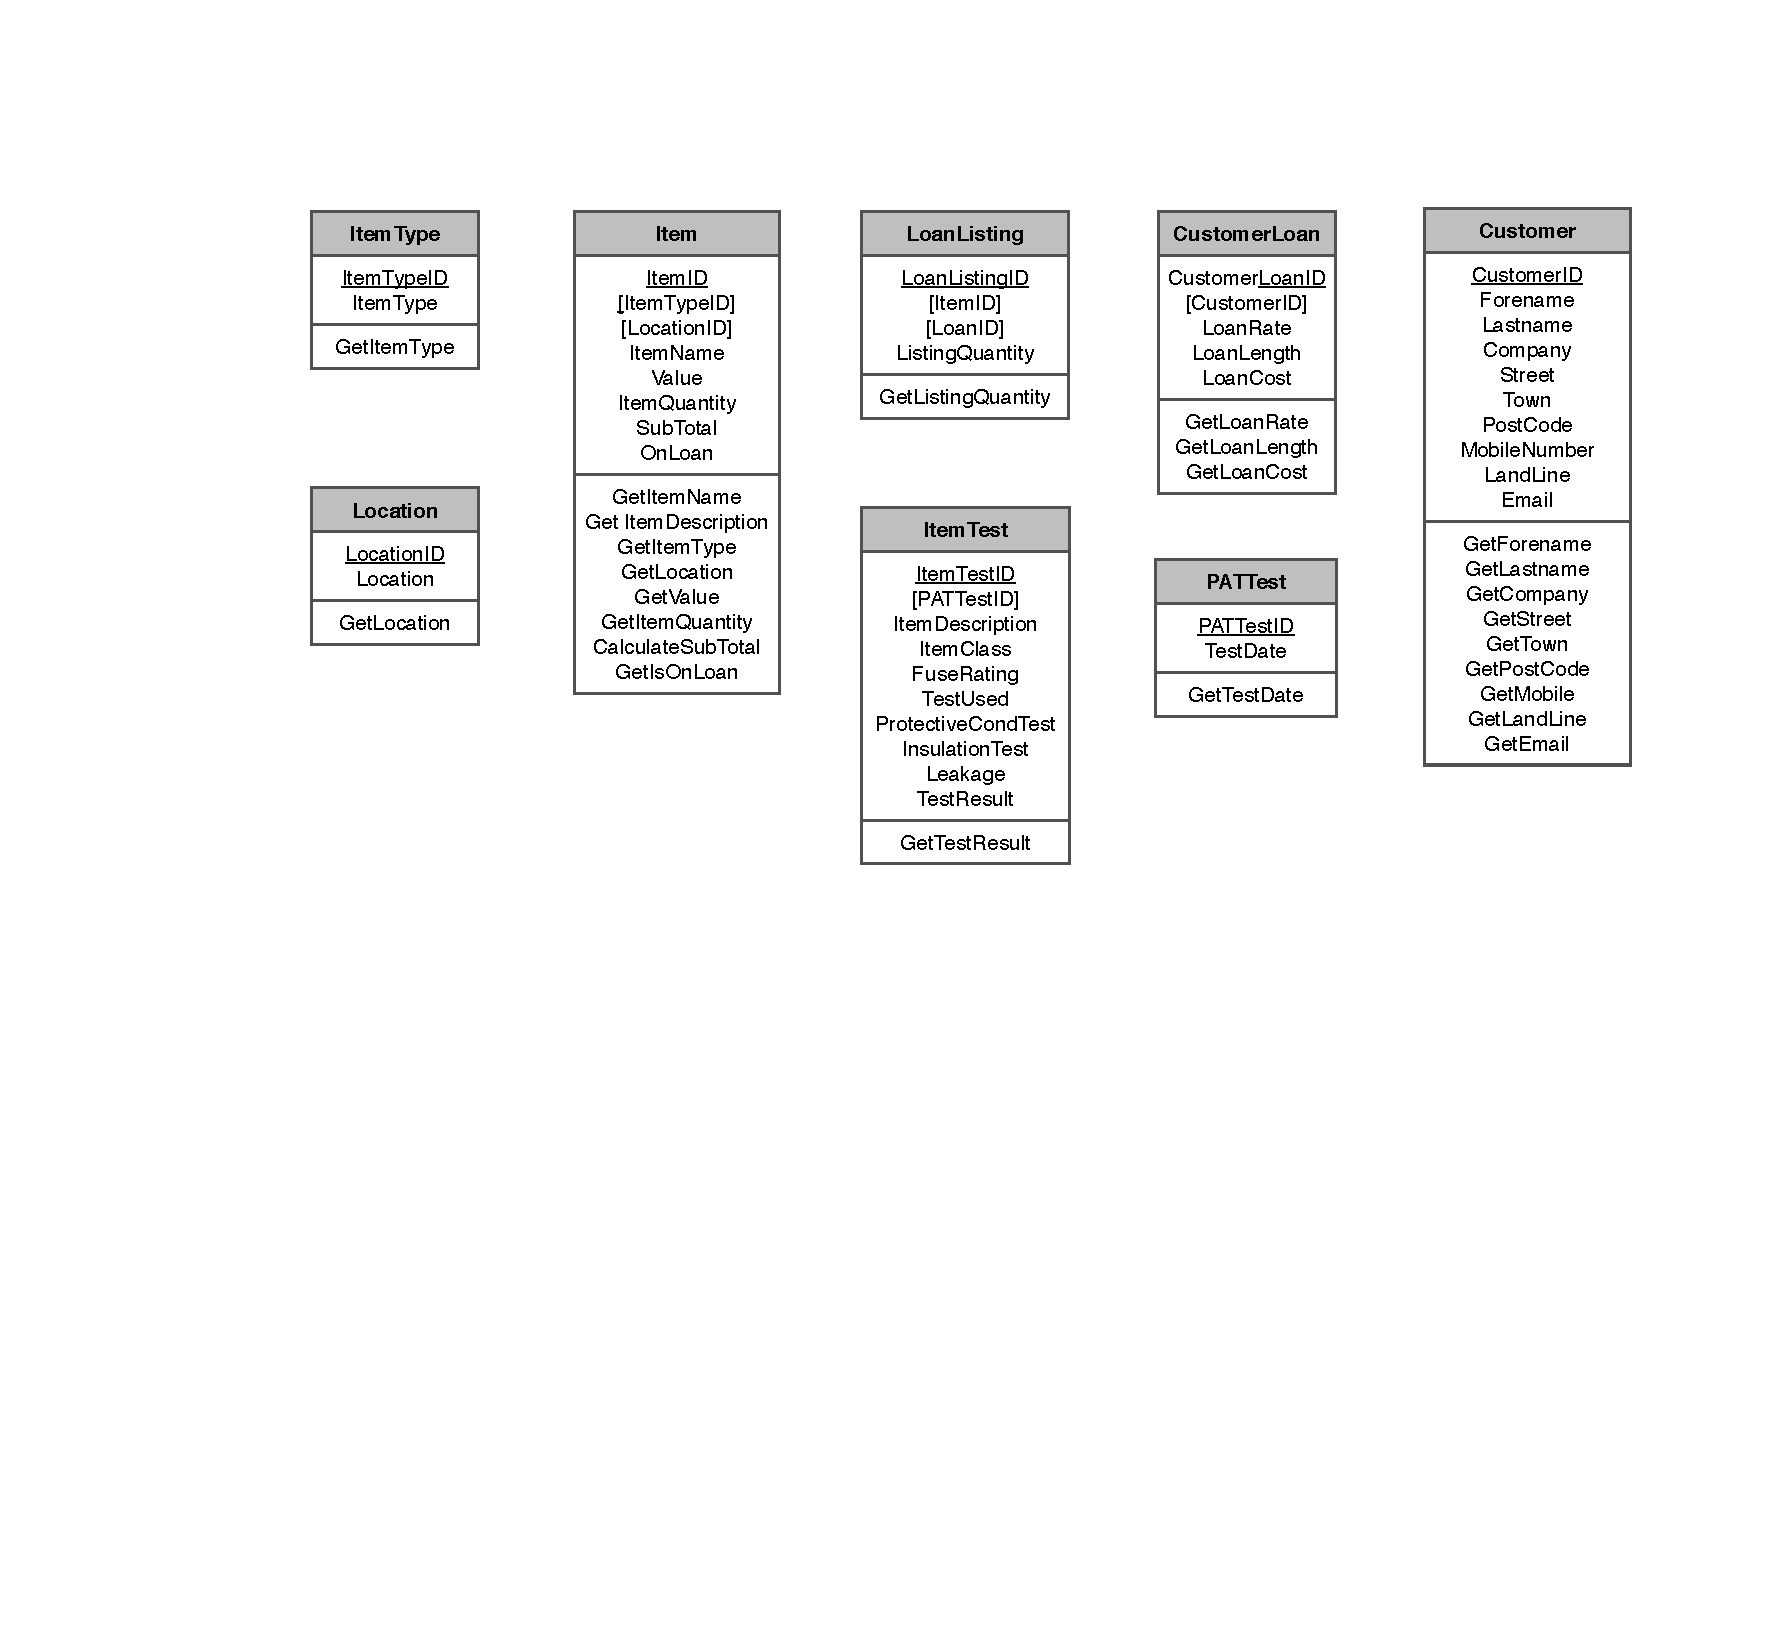
\includegraphics[width=450px]{./Design/Class_Definitions/Class_definitions.pdf}}
    \caption{Class Diagrams.} \label{fig:relationship_diagram}
\end{figure}


\end{landscape}

\newpage

\section{Prototyping}

\subsection{\textbf{Prototype for login interface}}
\begin{figure}[H]
    \centerline{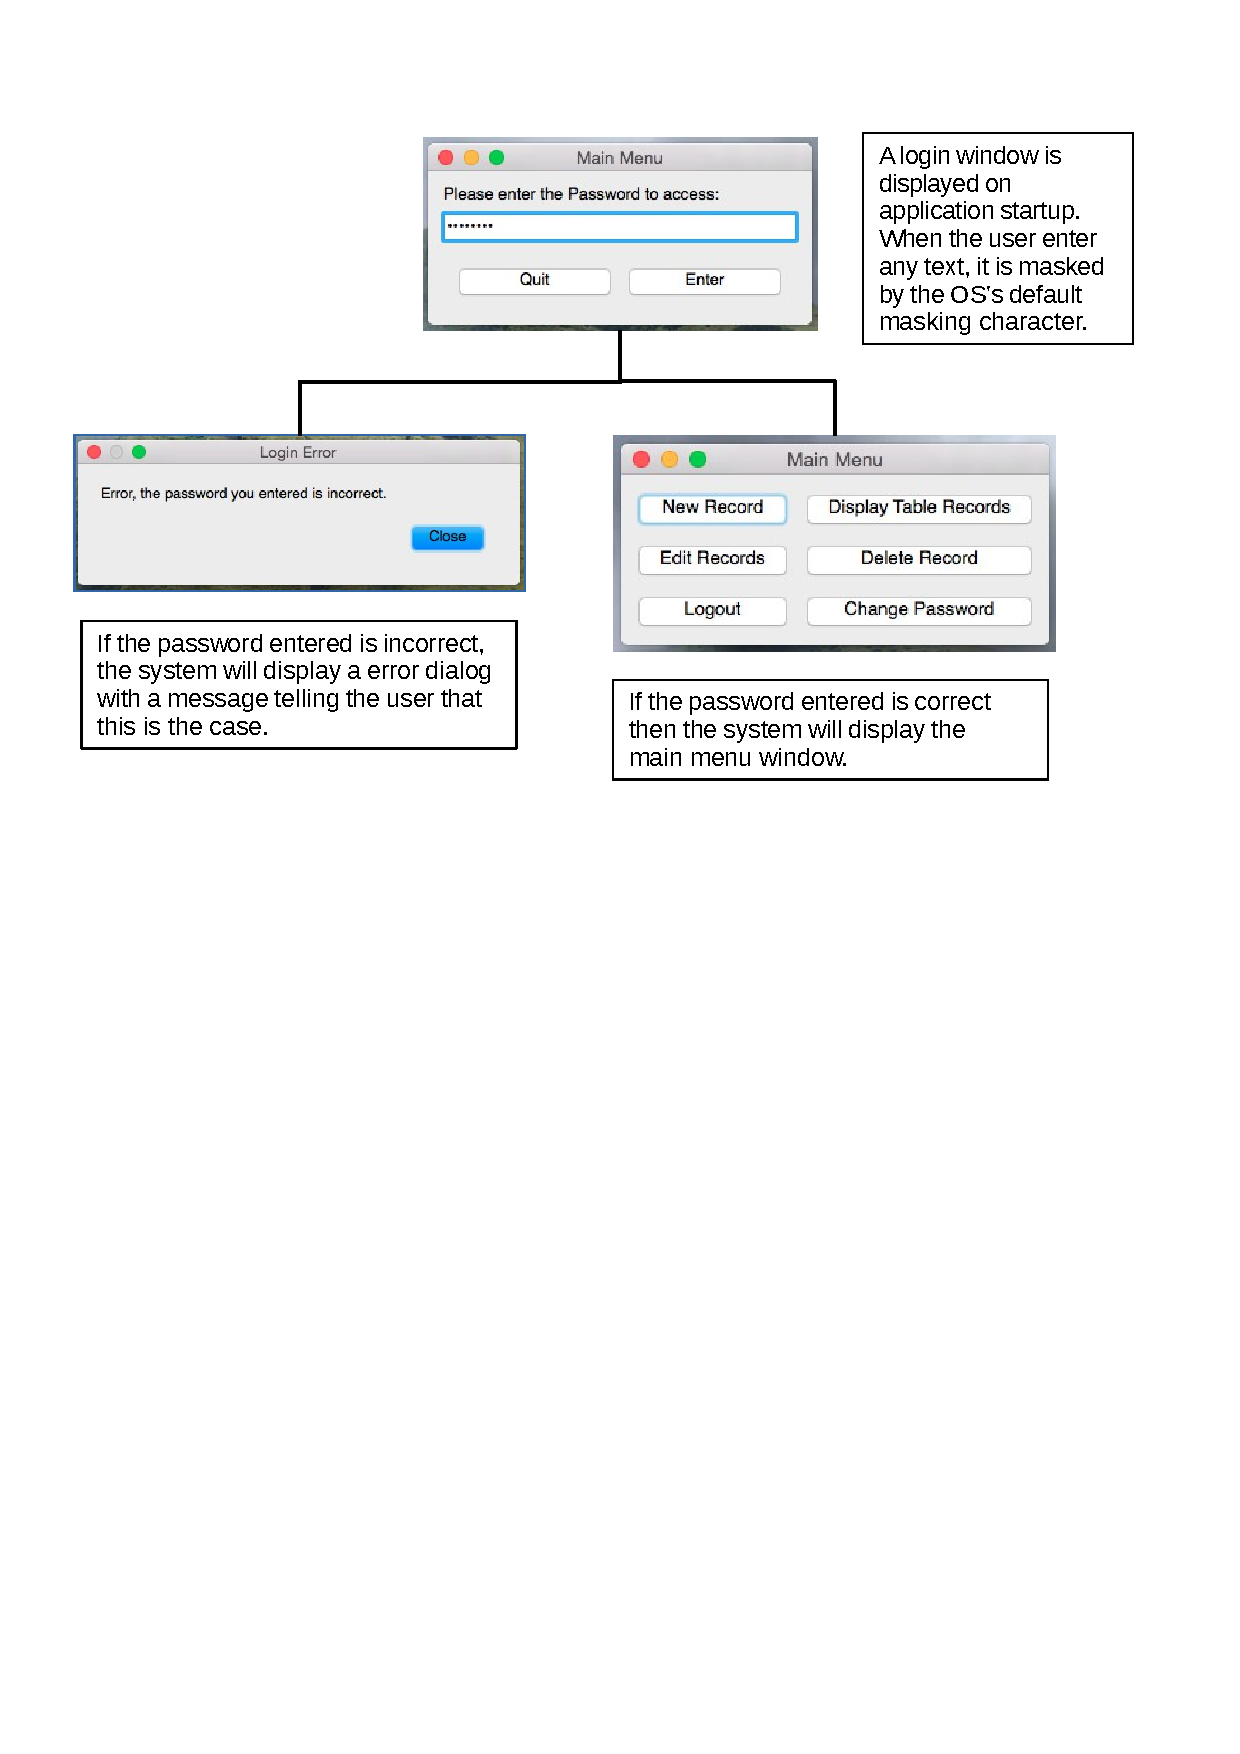
\includegraphics[width=300px]{./Design/Prototyping/Login_prototyping.pdf}}
    \caption{Login Prototype.} \label{fig:relationship_diagram}
\end{figure}

\subsection{\textbf{Prototype for change password interface}}
\begin{figure}[H]
    \centerline{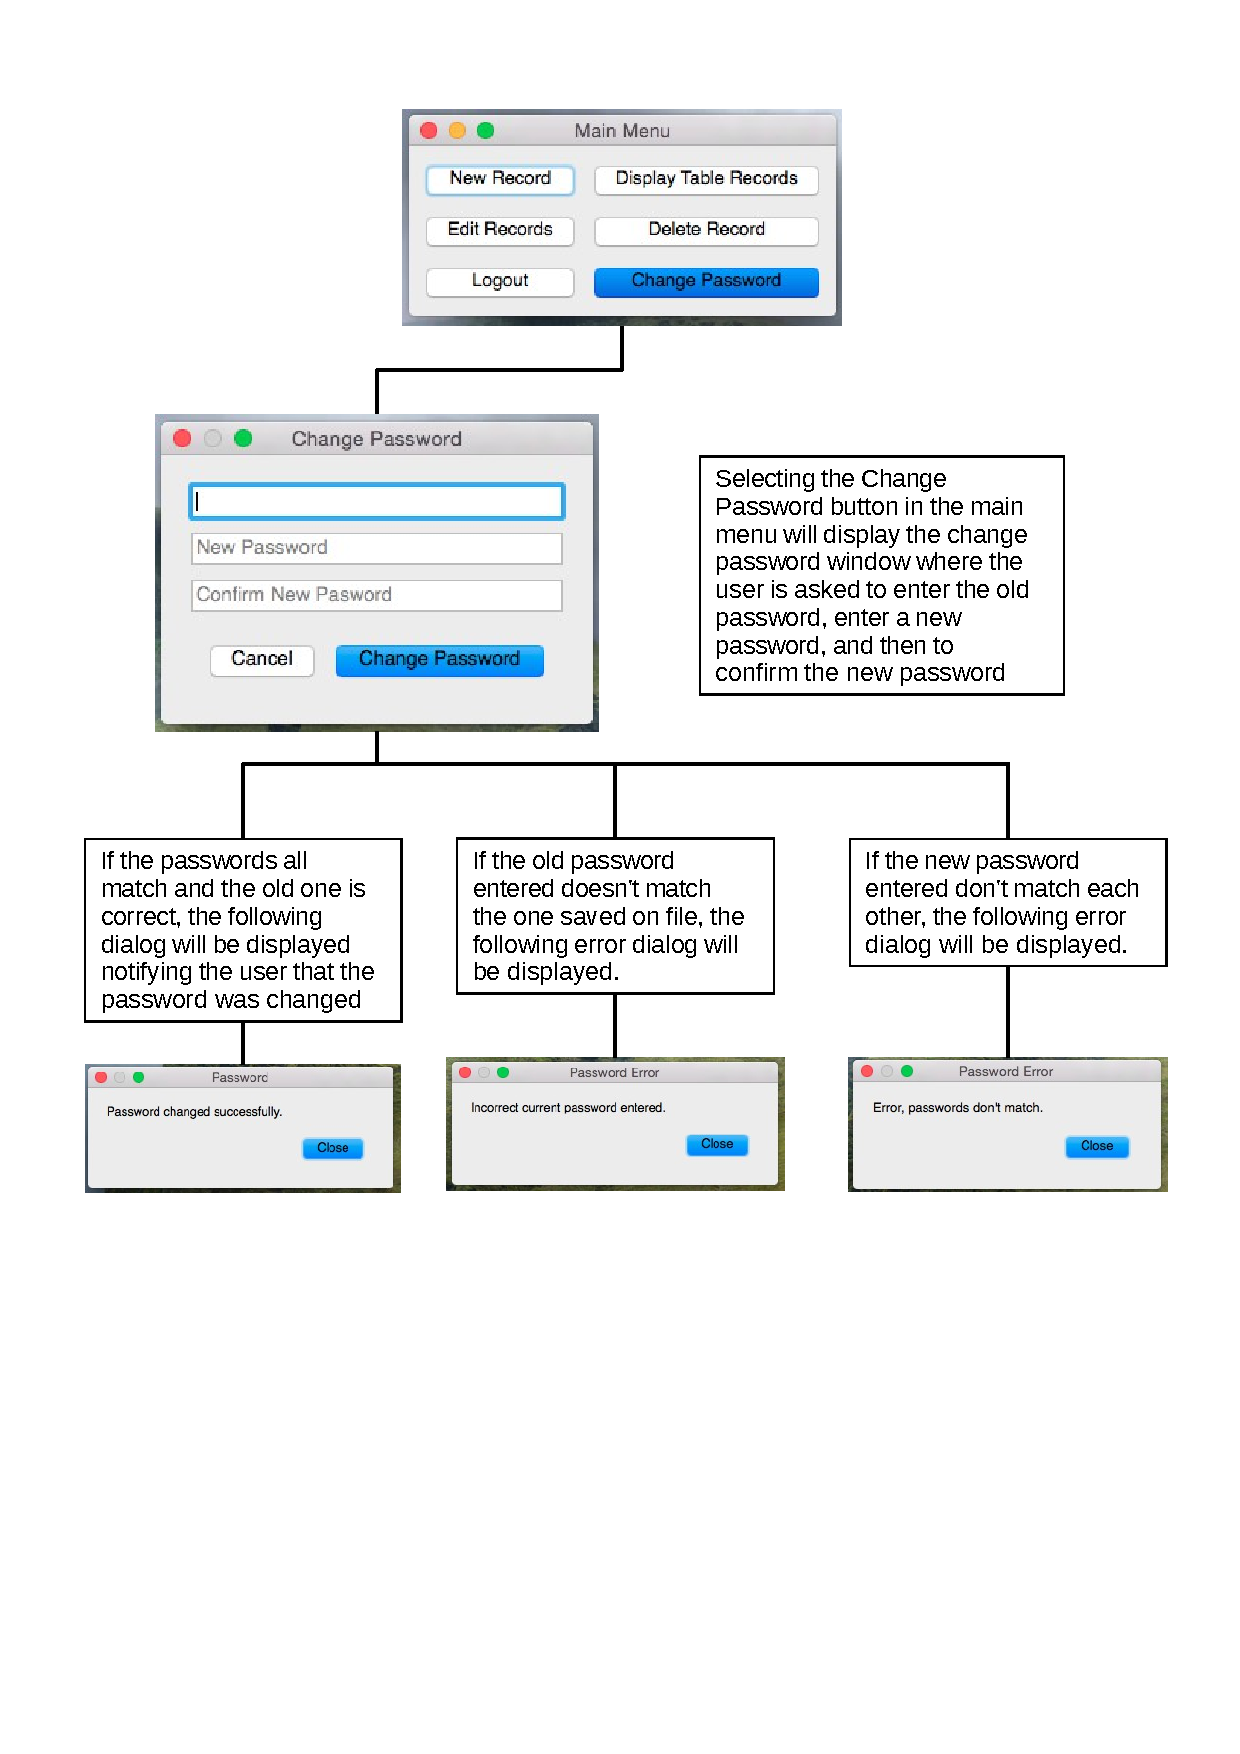
\includegraphics[width=250px]{./Design/Prototyping/Change_password_prototyping.pdf}}
    \caption{Change Password Prototype.} \label{fig:relationship_diagram}
\end{figure}

\subsection{\textbf{Prototype for printing interface}}
\begin{figure}[H]
    \centerline{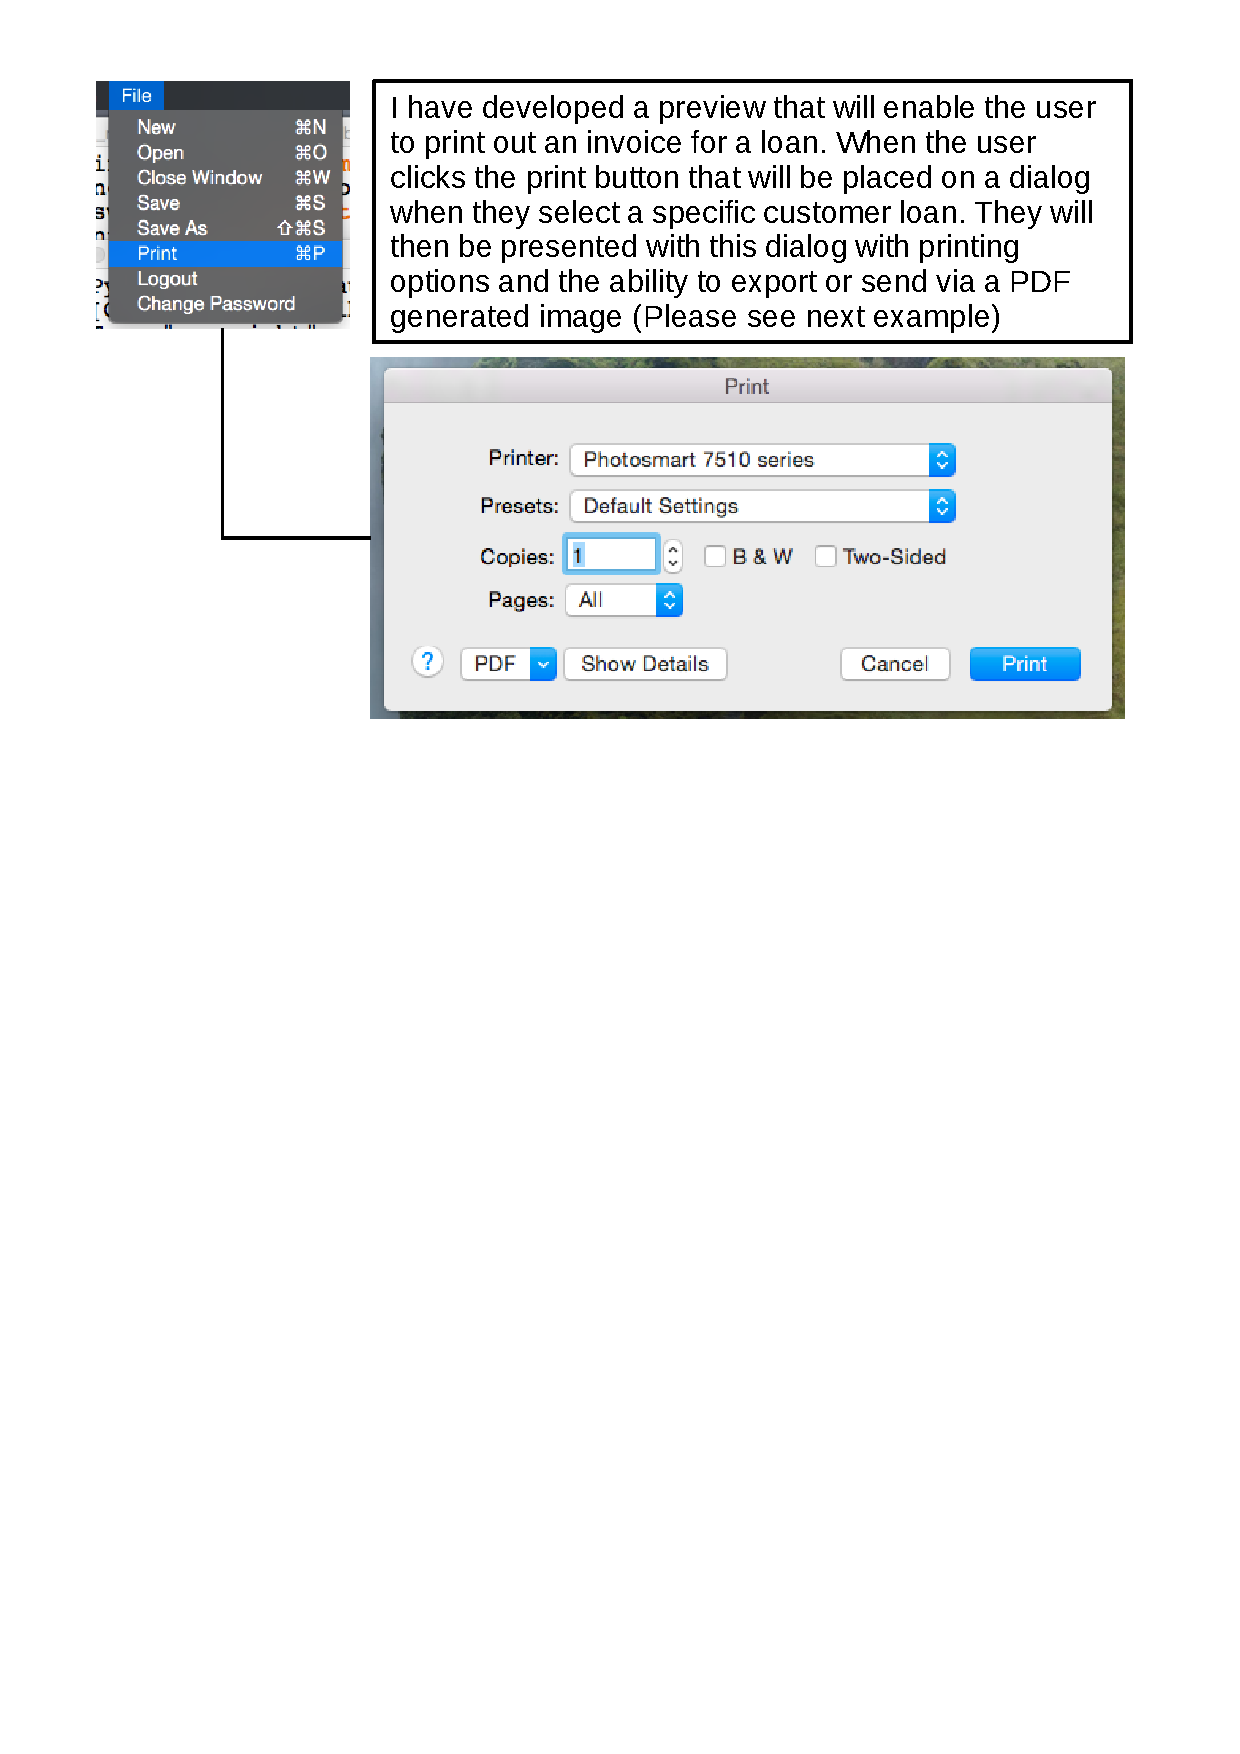
\includegraphics[width=300px]{./Design/Prototyping/Printing_prototyping.pdf}}
    \caption{Print Dialog.} \label{fig:relationship_diagram}
\end{figure}


\subsection{\textbf{Prototype for a loan invoice}}

\begin{figure}[H]
    \centerline{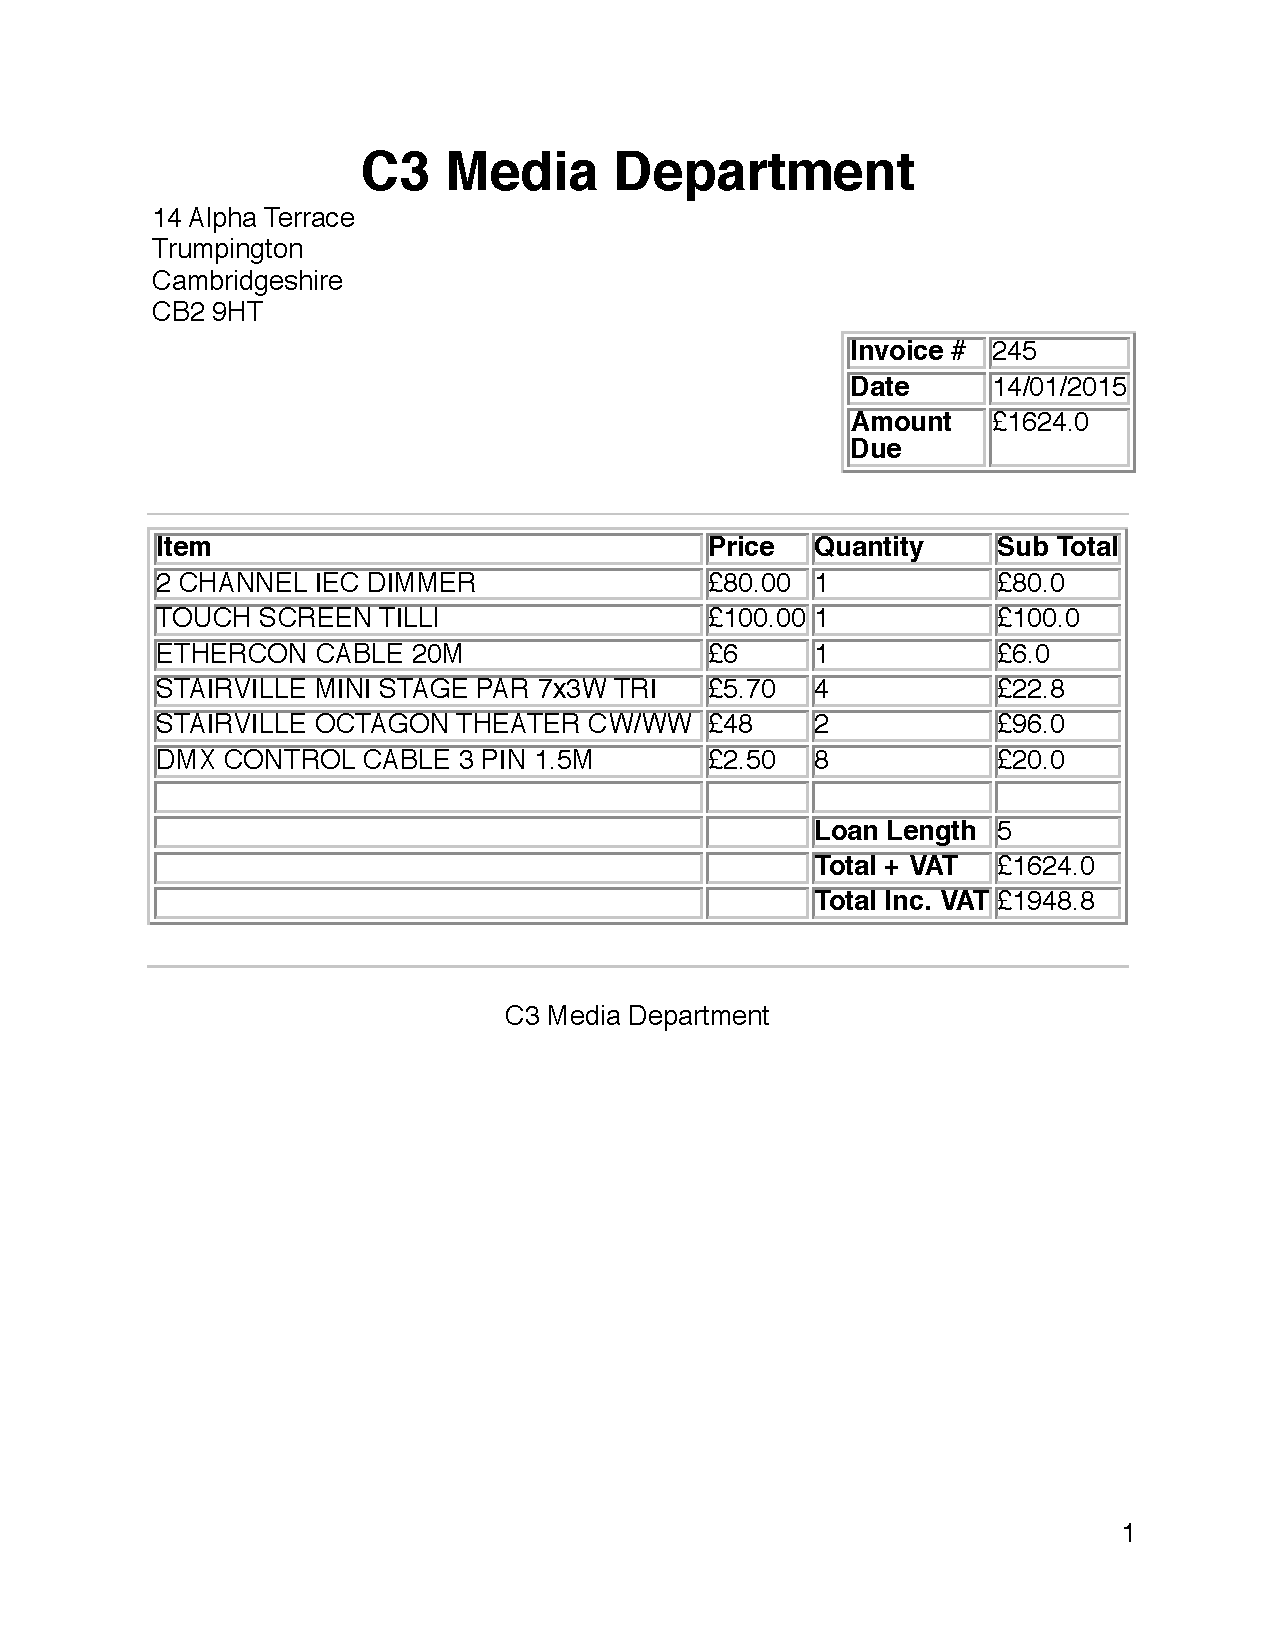
\includegraphics[width=400px]{./Design/Prototyping/invoice_preview.pdf}}
    \caption{PDF Invoice Prototype.} \label{fig:relationship_diagram}
\end{figure}

\section{Definition of Data Requirements}

\subsection{Identification of all data input items}

\begin{itemize}
    \item Item Name
    \item Item Value
    \item Loan Rate (The amount charged, per day, for the loan of the item)
    \item Item Class (This is the class for electric items and determines the type of PAT test it receives)
    \item Fuse Rating\\ \hline
    \item Start Date (The exact date a loan started)
    \item Loan Length (The length of the loan in days)
    \item Quantity (The quantity of an item to be loan out, if there is more than one in stock)\\ \hline
    \item Forename
    \item Surname
    \item Company
    \item Street
    \item Town
    \item Post Code
    \item Mobile Number
    \item Email Address
    \item Landline Number\\ \hline
    \item Test date (The date on which the PAT tests took place)
    \item Test Description (Notes referring to why an item failed or other notes about an individual item)
    \item Leakage (The current not obtained by an electrical item)
    \item Test Result (The result of the PAT test either Pass or Fail)
\end{itemize}

\subsection{Identification of all data output items}

\begin{itemize}
    \item Sub Total Cost (Loan Rate multiplied by the Quantity)
    \item Total Cost (The sum of all the Sub Total Costs in a single loan)\\
    \newline
    \textbf{\underline{Output to database}}
    \item Item Name
    \item Item Value
    \item Loan Rate (The amount charged, per day, for the loan of the item)
    \item Item Class (This is the class for electric items and determines the type of PAT test it receives)
    \item Fuse Rating\\ \hline
    \item Start Date (The exact date a loan started)
    \item Loan Length (The length of the loan in days)
    \item Quantity (The quantity of an item to be loan out, if there is more than one in stock)\\ \hline
    \item Forename
    \item Surname
    \item Company
    \item Street
    \item Town
    \item Post Code
    \item Mobile Number
    \item Email Address
    \item Landline Number\\ \hline
    \item Test date (The date on which the PAT tests took place)
    \item Test Description (Notes referring to why an item failed or other notes about an individual item)
    \item Leakage (The current not obtained by an electrical item)
    \item Test Result (The result of the PAT test either Pass or Fail)
\end{itemize}


\subsection{Explanation of how data output items are generated}

\begin{center}
    \begin{longtable}{|p{6cm}|p{6cm}|}
        \hline
        \textbf{Output}  & \textbf{How the output is generated} \\ \hline
        Sub Total Cost   & Calculated from LoanRate, Quantity and LoanLength \\ \hline
        Total Cost       & Calculated by adding all the Sub Total Costs in a Loan \\ \hline
        Item Name        & User Inputs the information \\ \hline
        Item Value       & User Inputs the information \\ \hline
        Loan Rate        & User Inputs the information \\ \hline
        Item Class       & User Inputs the information \\ \hline
        Fuse Rating      & User Inputs the information \\ \hline
        Start Date       & User Inputs the information \\ \hline
        Loan Length      & User Inputs the information \\ \hline
        Quantity         & User Inputs the information \\ \hline
        Forename         & User Inputs the information \\ \hline
        Surname          & User Inputs the information \\ \hline
        Company          & User Inputs the information \\ \hline
        Street           & User Inputs the information \\ \hline
        Town             & User Inputs the information \\ \hline
        Post Code        & User Inputs the information \\ \hline
        Mobile Number    & User Inputs the information \\ \hline
        Email Address    & User Inputs the information \\ \hline
        Landline Number  & User Inputs the information \\ \hline
        Test date        & User Inputs the information \\ \hline
        Test Description & User Inputs the information \\ \hline
        Leakage          & User Inputs the information \\ \hline
        Test Result      & User Inputs the information \\ \hline
    \end{longtable}

\end{center}


\begin{landscape}

    \begin{center}
    \subsection{Data dictionary}
    \end{center}
    
    \begin{center}
        \begin{tabular}{|p{3cm}|p{2cm}|p{3cm}|p{2cm}|p{2cm}|p{5cm}|}
            \hline
            \textbf{Name} & \textbf{Data Type} & \textbf{Length} & \textbf{Validation} & \textbf{Example Data} & \textbf{Comment} \\ \hline
            ItemTypeID & Integer & 1-435           & Range  & 253           & This is the \textbf{Primary Key} for the ItemType table, and \emph{Foreign Key} for the 
                                                                              Item table \\ \hline
            ItemType   & Text    & 5-40 Characters & Length & Computer      & This holds the description of each type of Item. \\ \hline
            LocationID & Integer & 1-3 Figures     & Range  & 3             & This is the \textbf{Primary Key} for the Location table and a \emph{Foreign Key} for the 
                                                                              Item table \\ \hline
            Location   & Text    & 1-30 Characters & Length & Main Offices  & This holds the name of the locations \\ \hline
            \end{tabular}
    \end{center}
\end{landscape}


\begin{landscape}
    \begin{center}
        \begin{tabular}{|p{3cm}|p{2cm}|p{3cm}|p{2cm}|p{2cm}|p{5cm}|}
            \hline
            \textbf{Name} & \textbf{Data Type} & \textbf{Length} & \textbf{Validation} & \textbf{Example Data} & \textbf{Comment} \\ \hline
            ItemID           & Integer & 1-435           & Range        & 253           & This is the \textbf{Primary Key} for the Item table, and \emph{Foreign Key} 
                                                                                          for the LoanItem and ItemTest tables \\ \hline
            ItemName         & Text    & 5-40 Characters & Length       & Arkaos Server & This gives the name of each item entered \\ \hline
            ItemValue        & Real    & 2-5 Figures     & Range        & 1,300         & This holds the data for the monetary value for each item \\ \hline
            LoanRate         & Real    & 2-5 Figures     & Range        & 7             & This holds the data for the monetary loan rate for each item \\ \hline
            ItemClass        & Integer & 1 Character     & Length       & 2             & A field to show what class of electrical equipment the item is \\ \hline
            FuseRating       & Text    & 1-3 Characters  & Length       & 5A            & A field which displays the fuse rating \\ \hline
            \end{tabular}
    \end{center}
\end{landscape}


\begin{landscape}
    \begin{center}
        \begin{tabular}{|p{3cm}|p{2cm}|p{3cm}|p{2cm}|p{2cm}|p{5cm}|}
            \hline
            \textbf{Name} & \textbf{Data Type} & \textbf{Length} & \textbf{Validation} & \textbf{Example Data} & \textbf{Comment} \\ \hline
            LoanID          & Integer & 1-435        & Range & 56  & This is the \textbf{Primary Key} for the Loan table and is a \emph{Foreign Key} in the Loan Item 
                                                                     table \\ \hline
            StartDate       & Real    & 1-5 Figures  & Range & 75  & Holds data displaying when the loan started \\ \hline
            LoanLength      & Integer & 1-3 Figures  & Range & 7   & Holds the data for the length of the loan \\ \hline
                            &         &              &       &     & \\ \hline
            LoanItemID      & Integer & 1-425        & Range & 26  & This is the \textbf{Primary Key} for the Loan Listings table \\ \hline
            Quantity        & Integer & 1-10         & Range & 3   & This hold data referring to the amount of one item has been loaned out \\ \hline
        \end{tabular}
    \end{center}
\end{landscape}


\begin{landscape}
    \begin{center}
        \begin{tabular}{|p{2.3cm}|p{2cm}|p{3cm}|p{2cm}|p{4.6cm}|p{4cm}|}
            \hline
            \textbf{Name} & \textbf{Data Type} & \textbf{Length} & \textbf{Validation} & \textbf{Example Data} & \textbf{Comment} \\ \hline
            CustomerID   & Integer & 1-255           & Range  & 52                     & This is the \textbf{Primary Key} for the Customer table \\ \hline
            Forename     & Text    & 3-20 Characters & Length & John                   & A field for the customers forename \\ \hline
            Lastname     & Text    & 3-20 Characters & Length & Smith                  & A field for the customers surname\\ \hline
            Company      & Text    & 3-20 Characters & Length & Digital Lighting Cambs & A field for the company's name\\ \hline
            Street       & Text    & 3-30 Characters & Length & 129 Cedar Crescent     & A field for the company's Street address\\ \hline
            Town         & Text    & 3-30 Characters & Length & Sawston                & A field for the company's Town \\ \hline
            County       & Text    & 3-20 Characters & Length & Cambs                  & A field for the company's County \\ \hline
            PostCode     & Text    & 6-7 Characters  & Format & CB22 7RX               & A field for the company's Postcode \\ \hline
            MobileNumber & Text    & 11 Characters   & Format & 07891234567            & A field for the customers mobile number\\ \hline
            LandLine     & Text    & 11 Characters   & Format & 01234567890            & A field for the customers landline phone \\ \hline
            Email        & Text    & 7-30 Characters & Length & john.smith@example.com & A field for the customers email address\\ \hline
        \end{tabular}
    \end{center}
\end{landscape}


\begin{landscape}
    \begin{center}
        \begin{tabular}{|p{3.4cm}|p{2cm}|p{2cm}|p{2cm}|p{4cm}|p{5cm}|}
            \hline
            \textbf{Name} & \textbf{Data Type} & \textbf{Length} & \textbf{Validation} & \textbf{Example Data} & \textbf{Comment} \\ \hline
            PATtestID          & Integer  & 1-255            & Range          & 52                  & This is the \textbf{Primary Key} for the PATtest table \\ \hline
            TestDate           & Date     & 10 Characters    & Format         & 01/12/2014          & A field that displays the date of the PAT test \\ \hline
             \\ \hline
            ItemTestID         & Integer  & 1-255            & Range          & 52                  & This is the \textbf{Primary Key} for the ItemTest table \\ \hline
            ItemDescription    & Text     & 3-400 Characters & Length         & Waltham portable TV & A field that describes the item to be tested \\ \hline
            ProtectiveCondTest & Float    & 4 Characters     & Length         & -                   & A field displaying the resistance of an item, in Ohms, to a 200mA 
                                                                                                      current  \\ \hline
            InsulationTest     & Text     & 3 Characters     & Length         & >20                 & A field displaying the Insulation of an item, in Ohms, to a 250V 
                                                                                                      or 500V Potential Difference \\ \hline
            Leakage            & Float    & 4 Characters     & Format         & 0.03                & A field that shows the current not obtained by the item, in 
                                                                                                     milliamperes \\ \hline
            TestResult         & Boolean  & -                & Presence Check & True                & A field to show if an item Passed or not\\ \hline
        \end{tabular}
    \end{center}
\end{landscape}

\subsection{Identification of appropriate storage media}

My system will not need to be accessed by more than 5 people, storing the database file on the server won't be necessary as everyone will then have access to the database file. Therefore, I have chosen to store the database file and application on a single machine which can be accessed by the people who need to use it at any time. The computer is in a central location and easily accessible by those who need to use it and has multiple hard disk drives which I can make use of for storage and backup. I will be using hard disk drives (HDD's) as my client already ownes them and they are cheaper than solid-state drives (SSD's).

\newpage

\begin{landscape}

\section{Database Design}

\subsection{ER Diagrams}

\begin{figure}[H]
    \centerline{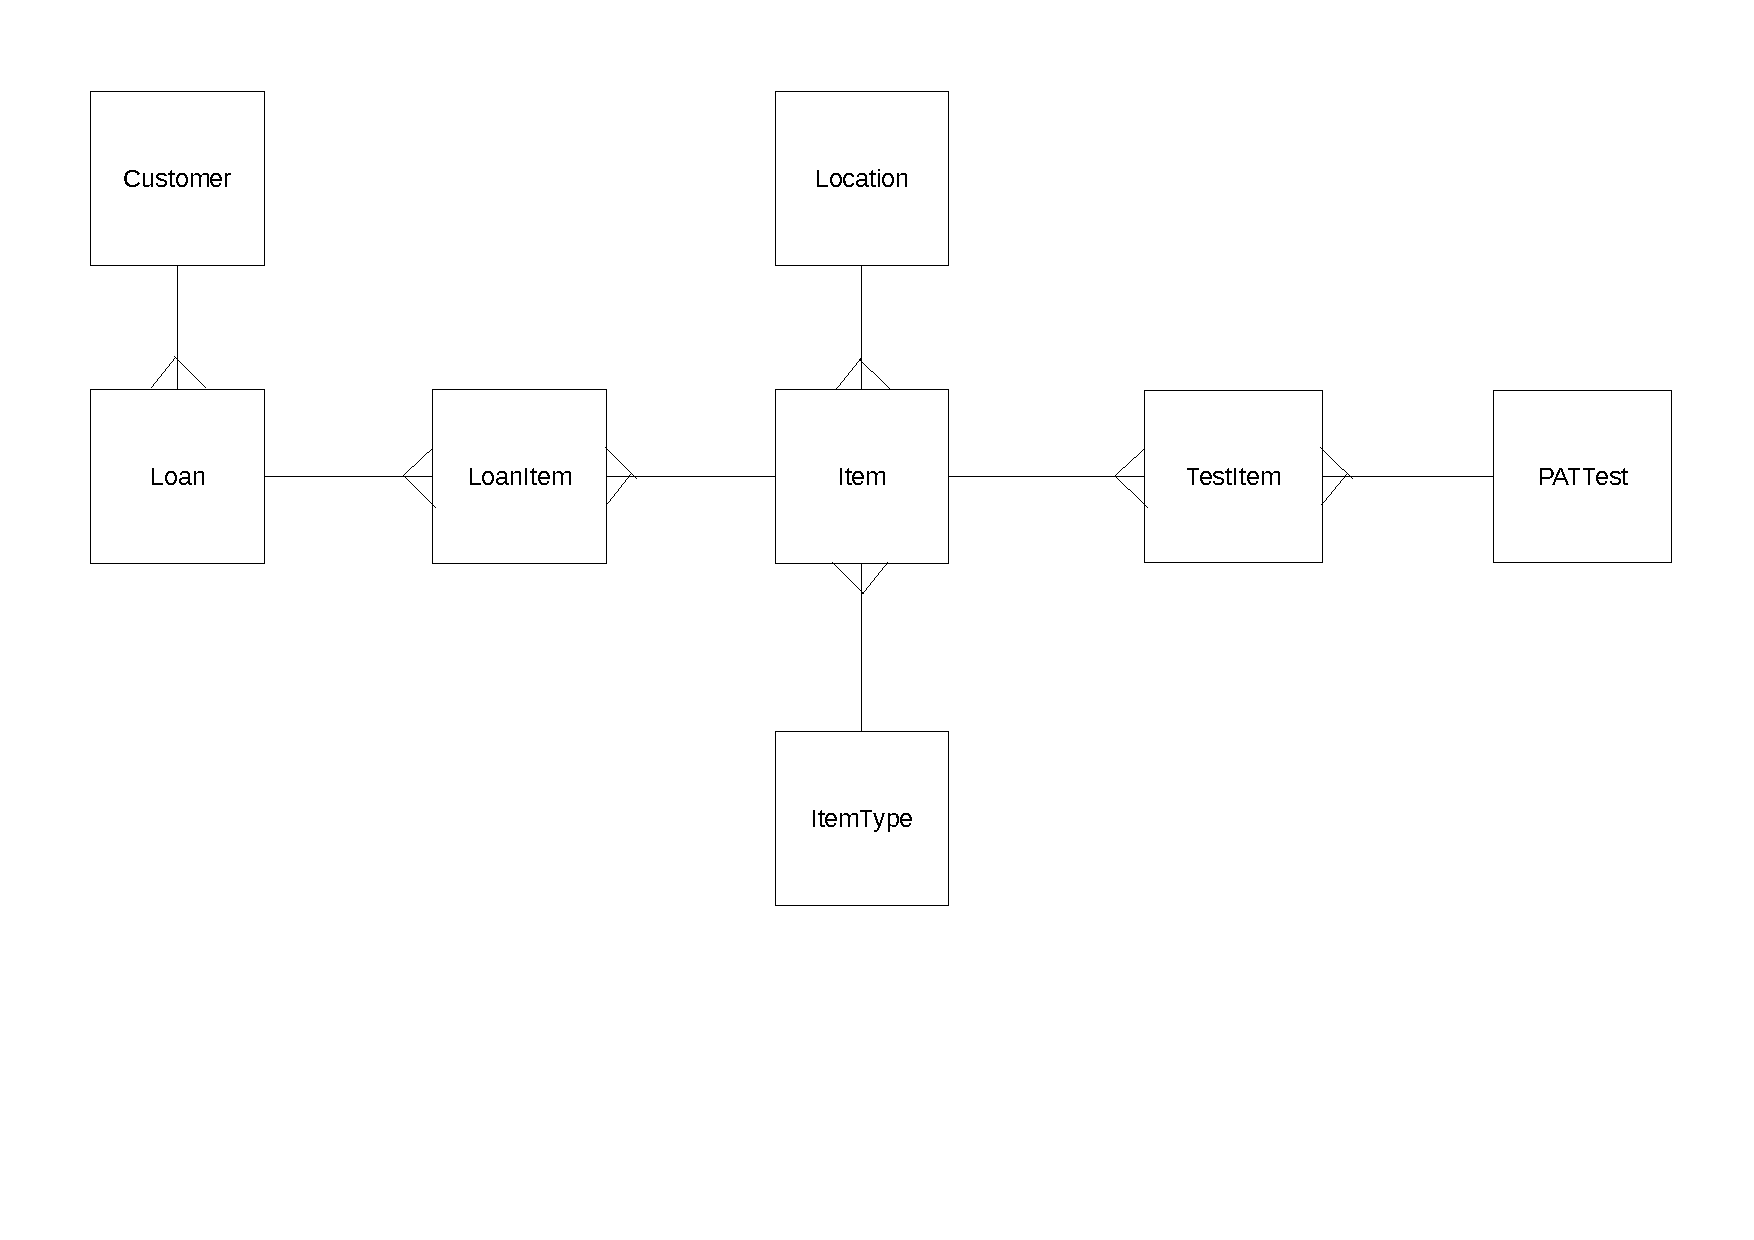
\includegraphics[width=550px]{./Design/ER_Diagrams/ER_Diagram.pdf}}
    \caption{ER Diagrams.} \label{fig:ER Diagrams}
\end{figure}

\end{landscape}

\subsection{Entity Descriptions}

\noindent \textbf{Location}(\underline{LocationID}, Location)

\noindent \textbf{ItemType}(\underline{ItemTypeID}, ItemType)

\noindent \textbf{Item}(\underline{ItemID}, ItemName, ItemValue, LoanRate, ItemClass, FuseRating,\\ \emph{ItemTypeID}, \emph{LocationID} )

\noindent \textbf{Customer}(\underline{CustomerID}, Forename, Surname, Company, Street, Town, PostCode, MobileNumber, Landline, Email)

\noindent \textbf{Loan}(\underline{LoanID}, \emph{CustomerID}, StartDate, LoanLength)

\noindent \textbf{LoanItem}(\underline{LoanItemID}, \emph{LoanID}, \emph{ItemID}, Quantity)

\noindent \textbf{PATtest}(\underline{PATtestID}, TestDate)

\noindent \textbf{ItemTest}(\underline{ItemTestID}, \emph{PATtestID}, \emph{ItemID}, PATtestNotes, ComponentType, ComponentResult, ComponentNotes, Leakage, TestResult)

\subsection{Normalisation}

\subsubsection{UNF to 3NF}

\begin{center}
    \begin{tabular}{|c|}
        \hline
        \textbf{Un-Normalised Form(UNF)}\\ \hline
        \underline{ItemID}              \\
        ItemName                        \\
        ItemType                        \\
        Location                        \\ 
        ItemValue                       \\ 
        LoanRate                        \\ 
        LoanID                          \\ 
        StartDate                       \\ 
        CustomerID                      \\ 
        Forename                        \\ 
        Lastname                        \\ 
        Company                         \\ 
        Street                          \\ 
        Town                            \\ 
        PostCode                        \\ 
        MobileNumber                    \\ 
        LandLine                        \\ 
        Email                           \\ 
        PATtestID                       \\
        TestResult                      \\ 
        TestDate                        \\ 
        ItemDescription                 \\ 
        ItemClass                       \\ 
        FuseRating                      \\ 
        PATTestNotes                    \\ 
        ComponentType                   \\
        ComponentResult                 \\
        ComponentNotes                  \\
        Leakage                         \\ \hline
    \end{tabular}
\end{center}

\newpage

\begin{center}
    \begin{tabular}{|c|c|}
        \hline
        \multicolumn{2}{|c|}{\textbf{First-Normalised Form(1NF)}} \\
        \multicolumn{2}{|c|}{ }                                   \\ \hline
        \textbf{Non-Repeating} & \textbf{Repeating}               \\ \hline
        \underline{ItemID}     & \underline{LoanID}               \\ 
        ItemName               & \emph{ItemID}                    \\ 
        ItemValue	          & StartDate                        \\ 
        LoanRate    	          & CustomerID                       \\ 
        ItemClass              & Forename                         \\ 
        FuseRating             & Lastname                         \\ 
              	              & Company                          \\ 
                               & Street                           \\ 
                               & Town                             \\ 
                               & PostCode                         \\ 
                               & MobileNumber                     \\ 
                               & Landline                         \\ 
                               & Email                            \\ 
                               & PATtestID                        \\ 
                               & TestDate                         \\ 
                               & PATTestNotes                     \\ 
                               & ComponentType                    \\
                               & ComponentResult                  \\
                               & ComponentNotes                   \\
                               & Leakage                          \\ 
                               & TestResult                       \\ \hline
    \end{tabular}
\end{center}

\newpage

\begin{center}
    \begin{tabular}{|c|c|}
        \hline
        \multicolumn{2}{|c|}{\textbf{Second-Normalised Form(2NF)}} \\
        \multicolumn{2}{|c|}{ }                                    \\ \hline
        \textbf{Non-Repeating} & \textbf{Repeating}                \\ \hline
        \underline{ItemID}     & \underline{LoanID}                \\ 
        ItemName               & \emph{ItemID}                     \\ 
        ItemValue	          & StartDate                         \\ 
        LoanRate 	          &                                   \\
        ItemClass              & \underline{CustomerID}            \\ 
        FuseRating             & Forename                          \\ 
                               & Lastname                          \\ 
              	              & Company                           \\ 
                               & Street                            \\ 
                               & Town                              \\ 
                               & PostCode                          \\ 
                               & MobileNumber                      \\ 
                               & Landline                          \\ 
                               & Email                             \\ 
                               & PATtestID                         \\ 
                               & TestDate                          \\ 
                               & PATTestNotes                      \\ 
                               & ComponentType                     \\
                               & ComponentResult                   \\
                               & ComponentNotes                    \\
                               & Leakage                           \\ 
                               & TestResult                        \\ 
                               & Location                          \\
                               & ItemType                          \\ \hline
    \end{tabular}
\end{center}

\begin{center}
    \begin{tabular}{|c|c|}
        \hline
        \multicolumn{2}{|c|}{\textbf{Third-Normalised Form(3NF)}}  \\
        \multicolumn{2}{|c|}{ }                                    \\ \hline
        \textbf{Non-Repeating}     & \textbf{Repeating}            \\ \hline
        \underline{ItemID}         & \underline{LoanID}            \\
        \emph{LocationID}          & \emph{CustomerID}             \\
        \emph{ItemTypeID}          & LoanLength                    \\
        ItemName                   &                               \\
        ItemValue	              &                               \\
        LoanRate                   & \underline{LoanItemID}        \\
        ItemClass                  & \emph{LoanID}                 \\
        FuseRating                 & \emph{ItemID}                 \\
                                   & Quantity                      \\
                                   &                               \\ 
                                   &\underline{CustomerID}         \\
                                   & Forename                      \\
                                   & Lastname                      \\ 
                                   & Company                       \\ 
                                   & Street                        \\ 
                                   & Town                          \\ 
                                   & PostCode                      \\ 
                                   & MobileNumber                  \\ 
                                   & Landline                      \\ 
                                   & Email                         \\ 
                                   &				                \\
                                   & \underline{PATtestID}         \\
                                   & TestDate                      \\   
                                   &				                \\
                                   & \underline{TestItem}          \\
                                   & \emph{PATtestID}              \\
                                   & \emph{ItemID}	                \\
                                   & PATTestNotes                  \\
                                   & ComponentType                 \\
                                   & ComponentResult               \\
                                   & ComponentNotes                \\
                                   & Leakage                       \\ 
                                   & TestResult                    \\ 
                                   &                               \\
                                   & \underline{LocationID}        \\
                                   & Location                      \\
                                   &                               \\
                                   & \underline{ItemTypeID}        \\
                                   & ItemType                      \\ \hline                                
    \end{tabular}
\end{center}

\section{SQL Queries}

\subsection{Get Items from Item Table}

\textbf{SQL query getting all the items from the Item table in the database ready to be formatted and displayed on screen}

\begin{sql}
      SELECT
      Item.ItemID,
      Item.ItemName,
      Item.ItemValue,
      Item.LoanRate,
      Item.ItemClass,
      Item.FuseRating,
      ItemType.ItemType,
      Location.Location
      FROM Item, ItemType, Location
      WHERE Item.LocationID = Location.LocationID AND Item.ItemTypeId = ItemType.ItemTypeID
\end{sql}

\subsection{Search Item Table for Items}

\textbf{SQL Query searching the database for Items by matching the item name, location or item type with a search string given by the user}

\begin{sql}
    SELECT 
    Item.ItemID,
    Item.ItemName,
    Item.ItemValue,
    ItemType.ItemType
    Location.Location
    FROM Item, ItemType, Location
    WHERE Item.ItemName LIKE '%'||:searchString||'%' OR Location.Location LIKE '%'||:searchString||'%'  OR ItemType.ItemType LIKE '%'||:searchString||'%' 
    AND LocationID = ? AND
    Location.LocationID = Item.LocationID
    ORDER BY ItemName ASC
\end{sql}

\subsection{Get Loans from Loan Table}

\textbf{SQL query getting all the Loans from the Loan table in the database ready to be formatted and displayed on screen}

\begin{sql}
    SELECT
    Loan.LoanID,
    Loan.StartDate,
    Loan.LoanLength,
    Customer.CustomerID,
    Customer.Company,
    FROM Loan, Customer
    WHERE Loan.CustomerID = Customer.CustomerID
\end{sql}

\subsection{Get all Loan Items from LoanItem Table}

\textbf{SQL query getting all the loan items from the LoanItem table in the database ready to be formatted and displayed on screen}

\begin{sql}
    SELECT
    LoanItem.LoanItemID,
    LoanItem.LoanID,
    LoanItem.Quantity,
    Item.ItemName,
    Item.LoanRate,
    FROM LoanItem, Item
    WHERE LoanItem.ItemID = Item.ItemID
\end{sql}

\newpage

\subsection{Search for loans taken out by a given Company}

\textbf{SQL Query searching the database to display Loans taken out by a certain person or company by matching the firstname or company fields with a search string entered by the user, ordered by date ascending}

\begin{sql}
    SELECT
    Loan.LoanID
    Customer.Company,
    Item.ItemName
    Item.LoanRate
    LoanItem.Quantity,
    Loan.StartDate,
    Loan.LoanLength,
    FROM Loan, Customer, Item
    WHERE Customer.FirstName LIKE '%'||:searchString||'%' OR Customer.Company LIKE '%'||:searchString3||'%' OR
    AND Customer.CustomerID = Loan.CustomerID AND Loan.LoanItemID = LoanItem.LoanItemID AND LoanItem.ItemID = Item.ItemID
    ORDER BY Loan.StartDate ASC
\end{sql}

\subsection{Get all Item Tests from ItemTest Table}

\textbf{SQL query getting all the Item Tests from the ItemTest table in the database ready to be formatted and displayed on screen}

\begin{sql}
      SELECT
      ItemTestID, 
      ItemTest.PATtestNotes,
      ItemTest.Leakage,
      ItemTest.TestResult,
      Item.ItemName,
      Item.ItemClass,
      Item.FuseRating
      FROM ItemTest
      WHERE ItemTest.ItemID = Item.ItemID
\end{sql}


\subsection{Search Customer Table for Customers}

\textbf{SQL Query searching the database for certain Customer Records by matching any of the text fields within the record with a search string specified by the user}

\begin{sql}
    SELECT * FROM Customer WHERE
	FirstName LIKE '%'||:searchString||'%' OR
	LastName LIKE '%'||:searchString2||'%' OR
	Company LIKE '%'||:searchString3||'%' OR
	Street LIKE '%'||:searchString4||'%' OR
	Town LIKE '%'||:searchString5||'%' OR
	County LIKE '%'||:searchString6||'%' OR
	PostCode LIKE '%'||:searchString7||'%' OR
	Mobile LIKE '%'||:searchString8||'%' OR
	Landline LIKE '%'||:searchString9||'%' OR
	Email LIKE '%'||:searchString10||'%'
\end{sql}

\newpage

\subsection{SQL Queries}

\section{Security and Integrity of the System and Data}

\subsection{Security and Integrity of Data}

The system will store personal data referring to an individual or a company. This data will fall under the data protection acts. This will mean that the data will need to be kept up to date and would therefore need a way to edit the data. All the information stored in the database should therefore be encrypted to keep this data secure and only accessible through my program which will be protected with a password. I will need to make sure the data stored is valid and correct, to do this I will need to use validation algorithms to make sure they are feasible.\\

\noindent I will also referential integrity in my database to make sure that when updating records such as Items, that the Location and ItemType records will not be affected by the changing of either LocationID or ItemTypeID in the Item table. This will take place in all the tables in the database that require foreign keys. I will use the "ON UPDATE CASCADE" SQL clause when updating the primary key of a record, records from other tables that use that primary key as a foreign key will also be updated.\\

\noindent Furthermore, I will use the "ON DELETE SET NULL" SQL clause as it will set the foreign key of any record to NULL if the record with that primary key has been deleted. This will be especially useful for the Location table as there will be temporary locations and the records that reference to a temporary location will not be deleted if the location is. This enables the user to back into the database and update the location.

\subsection{System Security}

It is important that the information in my database is secure and free from theft, corruption and tampering. This will be prevented with the use of a password to access the system. If the password that was entered is incorrect, the user will not be able to gain access to the system and will be notified by a pop-up window. I will need to encrypt my data to avoid people from outside my system from being able to access the data. All of the data entered into the system will undergo validation to make sure that it is suitable and correct.
Because some of the data fall under the data protection act, I will need to ensure that:
\begin{itemize}
    \item The data will be destroyed after 11 years of collection
    \item Only data that is necessary will be collected and stored.
    \item The data will be updated when necessary so that the data is up to date and accurate
    \item The data that is stored will only be used by the Church and not passed on to anyone else
    \item The data will be secured securely, to ensure that it is only accessed by authorised people
    \item The data will not be transferred to other countries
\end{itemize}


\section{Validation}

In order to insure that information is not entered incorrectly, the system will need to use certain validation methods in order to achieve appropriate data is input.

\begin{center}
    \begin{longtable}{|p{3cm}|p{2cm}|p{4cm}|p{4cm}|}
        \hline
        \textbf{Item}    & \textbf{Example} & \textbf{Validation or Verification Method} & \textbf{Comments}\\ \hline
        ItemName         & Asus PC Tower    & Presence check                             & Ensure a name is entered. No other validation 
                                                                                           needed as an ItemName can be any length\\ 
                                                                                           \hline
        ItemValue        & 400              & Presence check \newline Size Check         & Ensure a number is entered at that it is 
                                                                                           greater than 0\\ \hline
        LoanRate         & 7                & Presence Check                             & Ensure a value is entered that is 0 or greater
                                                                                           \\ \hline
        Item Class       & Multiple Choice  & Lookup Check \newline Presence Check       & Only two available Item Classes\\ \hline
        Fuse Rating      & 3A               & Presence Check                             & Ensure a value is entered\\ \hline
        Start Date       & 01/12/2014       & Presence Check                             & Ensures a date is entered\\ \hline
        Loan Length      & 7                & Presence Check                             & Ensures a valid value is entered and is 0 or 
                                                                                           greater\\ \hline
        Quantity         & 2                & Presence Check                             & Check that a value is entered \\ \hline
        Forename         & John             & Presence Check                             & Ensures a name is entered\\ \hline
        Surname          & Smith            & Presence Check                             & Ensures a name is entered\\ \hline
        Company          & Digital Inc      & Presence Check                             & Ensures a company is entered\\ \hline
        Street           & 10 Cedar Close   & Presence Check                             & Ensures a street is entered\\ \hline
        Town             & Great Shelford   & Presence Check                             & Ensures a town is entered\\ \hline
        Post Code        & AB12 4XY         & Presence Check \newline Type Check         & Ensures a postcode is entered and that it 
                                                                                           contains at least a number and a letter\\ 
                                                                                           \hline
        Mobile Number    & 01234567890      & Presence Check                             & Ensures a mobile number is entered and that it 
                                                                                           has a character length of 11\\ \hline
        Email Address    & example@url.com  & Presence Check \newline Type Check         & Ensures an email is entered and that it 
                                                                                           contains the characters '@' and '.'\\ \hline
        Landline Number  & 01234567890      & Presence Check                             & Ensures a mobile number is entered and that it 
                                                                                           has a character length of 11\\ \hline
        Test date        & 01/12/2014       & Presence Check                             & Ensures a date is entered\\ \hline
        Test Result      & yes              & Presence Check                             & Ensures that a yes or no is entered. This is 
                                                                                           converted to a boolean\\ \hline
        Password         & p4assw0rd        & Presence Check \newline Type Check         & Ensures a password is entered and that it 
                                                                                           contains a letter and a number\\ \hline
    \end{longtable}

\end{center}


\begin{landscape}

\section{Testing}

\subsection{Outline Plan}

\begin{center}
    \begin{tabular}{|p{3cm}|p{3.5cm}|p{4cm}|p{6cm}|}
        \hline
        \textbf{Test Series} & \textbf{Purpose of Test Series} & \textbf{Testing Strategy} & \textbf{Strategy Rationale}\\ \hline
        1 & Test the flow of control between interfaces      & Top-down testing     & To make sure that user interfaces interact correctly and don't present graphical glitches or bugs\\ \hline
        2 & Test data input validation works                 & Botton-up testing    & Testing of each component will commence when they have been developed\\ \hline
        3 & Test data input is stored correctly              & Black box testing    & Ensure that data input by the user is stored at the correct locations within the database\\ \hline
        4 & Test Algorithms and check output is correct      & White box testing    & Make sure calculations such as loan costs are calculated correctly when including VAT\\ \hline
        5.& Test system meets requirements                   & Acceptance Testing   & Make sure the system meets the all the clients expectations and fulfils all primary objectives\\ \hline
    \end{tabular}
\end{center}

\newpage

\subsection{Detailed Plan}

\begin{center}
    \begin{longtable}{|p{1.5cm}|p{2cm}|p{3cm}|p{2cm}|p{2cm}|p{2.5cm}|p{2cm}|p{2cm}|}
        \hline
        \textbf{Test Series} & \textbf{Purpose of Test} & \textbf{Test Description} & \textbf{Test Data} & \textbf{Test Data Type (Normal/ Erroneous/ Boundary)} & \textbf{Expected Result} & \textbf{Actual Result} & \textbf{Evidence}\\ \hline
        
        1.01 & Test the "Login" button functions correctly & This should link to the main menu screen & Enter "password" and click the "Login" button & Normal & The 
        main menu window should be displayed  & & \\ \hline
        
        1.02 & Test the "Logout" button functions correctly & This should link back to the login screen & Click "Logout" button & Normal & The login screen should 
        be displayed & & \\ \hline
        
        1.03 & Test the "Change Password" functions correctly & This should link to the Change password dialog window & Click "Change Password" button & Normal & The 
        change password window should be displayed & & \\ \hline
        
        1.04 & Test the and "Cancel" buttons functions correctly & This should link back to the main menu window & Click "Cancel" button & Normal & The main menu should 
        be displayed & & \\ \hline
        
        1.05 & Test the "Confirm Password" button functions correctly & This should link to a message dialog confirming that the password has been changed, other 
        messages will be displayed if the current password is incorrect or the new passwords don't match & Click the "Confirm Password" button & Normal & The message 
        dialog window should be displayed & & \\ \hline
        
        1.06 & Test the "OK" button on the message dialog functions correctly & This should link back to the main menu window & Click the "OK" button & Normal & The 
        main menu window should be displayed & & \\ \hline
        
        1.07 & Test the enter record button functions correctly & This should link to a table selection window & Click "Enter Record" button & Normal & The table
        selection dialog box should be displayed & & \\ \hline 
        
        1.08 & Test the table selection dialog function correctly on selecting the Item table & This should link to the enter item record window & Select "Item Table" 
        and click "Enter Record" & Normal & The enter Item Record Window should be displayed & & \\ \hline
        
        1.09 & Test the table selection dialog function correctly on selecting the Customer table & This should link to the enter customer record window & Select 
        "Customer Table" and click "Enter Record" & Normal & The enter Customer Record Window should be displayed & & \\ \hline

        1.10 & Test the table selection dialog function correctly on selecting the Loan table & This should link to the enter loan record window & Select "Loan 
        Table" and click "Enter Record" & Normal & The enter Loan Record Window should be displayed & & \\ \hline
        
        1.10 & Test the table selection dialog function correctly on selecting the PAT test table & This should link to the enter PAT test record window & Select "PAT 
        test Table" and click "Enter Record" & Normal & The enter PAT test Record Window should be displayed & & \\ \hline
        
        1.11 & Check that the "Confirm" button functions correctly on the enter Item record window & This should link back to the main menu & Select the "Confirm" 
        button & Normal & The main window should be displayed & & \\ \hline
        
        1.12 & Check that the "Confirm" button functions correctly on the enter Customer record window & This should link back to the main menu & Select the "Confirm" 
        button & Normal & The main window should be displayed & & \\ \hline
        
        1.13 & Check that the "Confirm" button functions correctly on the enter Loan record window & This should link back to the main menu & Select the "Confirm" 
        button & Normal & The main window should be displayed & & \\ \hline
        
        1.14 & Check that the "Confirm" button functions correctly on the enter PAT test record window & This should link back to the main menu & Select the "Confirm" 
        button & Normal & The main window should be displayed & & \\ \hline
        
        1.15 & Check that the "Cancel" button functions correctly on the enter Item record window & This should link back to the main menu & Select the "Cancel" 
        button & Normal & The table selection window should be displayed & & \\ \hline
        
        1.16 & Check that the "Cancel" button functions correctly on the enter Customer record window & This should link back to the main menu & Select the "Cancel" 
        button & Normal & The table selection window should be displayed & & \\ \hline
        
        1.17 & Check that the "Cancel" button functions correctly on the enter Loan record window & This should link back to the main menu & Select the "Cancel" 
        button & Normal & The table selection window should be displayed & & \\ \hline
        
        1.18 & Check that the "Cancel" button functions correctly on the enter PAT test record window & This should link back to the main menu & Select the "Cancel" 
        button & Normal & The table selection window should be displayed & & \\ \hline
        
        1.19 & Test the "Display Records" button functions correctly & This should link to a table selection window & Click "Display Records" button & Normal & The 
        table selection dialog box should be displayed & & \\ \hline 

        1.20 & Test the table selection dialog function correctly on selecting the Item table & This should link to the display item records window & Select "Item 
        Table" and click "Display Record" & Normal & The enter Item Record Window should be displayed & & \\ \hline
        
        1.21 & Test the display Item records "Search" button functions correctly & This should link to the search dialog & Click the "Search" button & Normal & The 
        search dialog should be displayed & & \\ \hline
        
        1.22 & Test the search dialogs "Search" button functions correctly & This should link to a dialog window displaying the found record or a dialog window 
        displaying a message that the record wasn't found & Click the "Search" button & Normal & The appropriate dialog should be displayed if a record was found or not
         & & \\ \hline
        
        1.23 & Test the table selection dialog function correctly on selecting the Customer table & This should link to the display customer records window & Select 
        "Customer Table" and click "Display Record" & Normal & The enter Customer Record Window should be displayed & & \\ \hline
        
        1.24 & Test the display Customer records "Search" button functions correctly & This should link to the search dialog & Click the "Search" button & Normal & The 
        search dialog should be displayed & & \\ \hline
        
        1.25 & Test the search dialogs "Search" button functions correctly & This should link to a dialog window displaying the found record or a dialog window 
        displaying a message that the record wasn't found & Click the "Search" button & Normal & The appropriate dialog should be displayed if a record was found or not
         & & \\ \hline

        1.26 & Test the table selection dialog function correctly on selecting the Loan table & This should link to the display item loan records window & Select "Loan 
        Table" and click "Display Record" & Normal & The enter Loan Record Window should be displayed & & \\ \hline
        
        1.27 & Test the display loan records "Search" button functions correctly & This should link to the search dialog & Click the "Search" button & Normal & The 
        search dialog should be displayed & & \\ \hline
        
        1.28 & Test that the display loan records "Print" button functions correctly & This should link to the print dialog box & Click the "Print" button & Normal & 
        The print dialog box should be displayed & & \\ \hline
        
        1.28 & Test the search dialogs "Search" button functions correctly & This should link to a dialog window displaying the found record or a dialog window 
        displaying a message that the record wasn't found & Click the "Search" button & Normal & The appropriate dialog should be displayed if a record was found or not
         & & \\ \hline
        
        1.29 & Test the table selection dialog function correctly on selecting the PAT test table & This should link to the display PAT test records window & Select 
        "PAT test Table" and click "Display Record" & Normal & The enter PAT test Record Window should be displayed & & \\ \hline
        
        1.30 & Test the display PAT test records "Search" button functions correctly & This should link to the search dialog & Click the "Search" button & Normal & The 
        search dialog should be displayed & & \\ \hline
        
        1.31 & Test the search dialogs "Search" button functions correctly & This should link to a dialog window displaying the found record or a dialog window 
        displaying a message that the record wasn't found & Click the "Search" button & Normal & The appropriate dialog should be displayed if a record was found or not
         & & \\ \hline
         
        1.32 & Test the edit record button functions correctly & This should link to a table selection window & Click "Edit Record" button & Normal & The table
        selection dialog box should be displayed & & \\ \hline 
        
        1.33 & Test the table selection dialog function correctly on selecting the Item table & This should link to the edit item record window & Select "Item Table" 
        and click "Edit Record" & Normal & The edit Item Record Window should be displayed & & \\ \hline
        
        1.34 & Test the table selection dialog function correctly on selecting the Customer table & This should link to the edit customer record window & Select 
        "Customer Table" and click "Edit Record" & Normal & The edit Customer Record Window should be displayed & & \\ \hline

        1.35 & Test the table selection dialog function correctly on selecting the Loan table & This should link to the edit loan record window & Select "Loan 
        Table" and click "Edit Record" & Normal & The edit Loan Record Window should be displayed & & \\ \hline
        
        1.36 & Test the table selection dialog function correctly on selecting the PAT test table & This should link to the edit PAT test record window & Select "PAT 
        test Table" and click "Edit Record" & Normal & The edit PAT test Record Window should be displayed & & \\ \hline
        
        1.37 & Check that the "Confirm" button functions correctly on the edit Item record window & This should link back to the main menu & Select the "Confirm" 
        button & Normal & The main window should be displayed & & \\ \hline
        
        1.38 & Check that the "Confirm" button functions correctly on the edit Customer record window & This should link back to the main menu & Select the "Confirm" 
        button & Normal & The main window should be displayed & & \\ \hline
        
        1.39 & Check that the "Confirm" button functions correctly on the edit Loan record window & This should link back to the main menu & Select the "Confirm" 
        button & Normal & The main window should be displayed & & \\ \hline
        
        1.40 & Check that the "Confirm" button functions correctly on the edit PAT test record window & This should link back to the main menu & Select the "Confirm" 
        button & Normal & The main window should be displayed & & \\ \hline
        
        1.41 & Check that the "Cancel" button functions correctly on the edit Item record window & This should link back to the main menu & Select the "Cancel" 
        button & Normal & The table selection window should be displayed & & \\ \hline
        
        1.42 & Check that the "Cancel" button functions correctly on the edit Customer record window & This should link back to the main menu & Select the "Cancel" 
        button & Normal & The table selection window should be displayed & & \\ \hline
        
        1.43 & Check that the "Cancel" button functions correctly on the edit Loan record window & This should link back to the main menu & Select the "Cancel" 
        button & Normal & The table selection window should be displayed & & \\ \hline
        
        1.44 & Check that the "Cancel" button functions correctly on the edit PAT test record window & This should link back to the main menu & Select the "Cancel" 
        button & Normal & The table selection window should be displayed & & \\ \hline
        
        1.45 & Test the delete record button functions correctly & This should link to a table selection window & Click "Delete Record" button & Normal & The table
        selection dialog box should be displayed & & \\ \hline 
        
        1.46 & Test the table selection dialog function correctly on selecting the Item table & This should link to the delete item record window & Select "Item Table" 
        and click "Delete Record" & Normal & The edit Item Record Window should be displayed & & \\ \hline
        
        1.47 & Test the table selection dialog function correctly on selecting the Customer table & This should link to the delete customer record window & Select 
        "Customer Table" and click "Delete Record" & Normal & The edit Customer Record Window should be displayed & & \\ \hline

        1.48 & Test the table selection dialog function correctly on selecting the Loan table & This should link to the delete loan record window & Select "Loan 
        Table" and click "Delete Record" & Normal & The edit Loan Record Window should be displayed & & \\ \hline
        
        1.49 & Test the table selection dialog function correctly on selecting the PAT test table & This should link to the delete PAT test record window & Select "PAT 
        test Table" and click "Delete Record" & Normal & The edit PAT test Record Window should be displayed & & \\ \hline
        
        1.50 & Check that the "Confirm" button functions correctly on the delete Item record window & This should link back to the main menu & Select the record(s) for 
        delete and click "Confirm" button & Normal & The main window should be displayed & & \\ \hline
        
        1.51 & Check that the "Confirm" button functions correctly on the delete Customer record window & This should link back to the main menu & Select the record(s) 
        for delete and click "Confirm" button & Normal & The main window should be displayed & & \\ \hline
        
        1.52 & Check that the "Confirm" button functions correctly on the delete Loan record window & This should link back to the main menu & Select the record(s) for 
        delete and click "Confirm" button & Normal & The main window should be displayed & & \\ \hline
        
        1.53 & Check that the "Confirm" button functions correctly on the delete PAT test record window & This should link back to the main menu & Select the record(s) 
        for delete and click "Confirm" button & Normal & The main window should be displayed & & \\ \hline
        
        1.54 & Check that the "Cancel" button functions correctly on the delete Item record window & This should link back to the main menu & Click the "Cancel" 
        button & Normal & The table selection window should be displayed & & \\ \hline
        
        1.55 & Check that the "Cancel" button functions correctly on the delete Customer record window & This should link back to the main menu & Click the "Cancel" 
        button & Normal & The table selection window should be displayed & & \\ \hline
        
        1.56 & Check that the "Cancel" button functions correctly on the delete Loan record window & This should link back to the main menu & Click the "Cancel" 
        button & Normal & The table selection window should be displayed & & \\ \hline
        
        1.57 & Check that the "Cancel" button functions correctly on the delete PAT test record window & This should link back to the main menu & Click the "Cancel" 
        button & Normal & The table selection window should be displayed & & \\ \hline
        
        & & & & & & & \\ \hline
        
        2.01 & Verify that a password was entered & An error dialog box should appear if no password is entered & "password" & Normal & Accepted & & \\
             &                                    &                                                             &  nothing   & erroneous & Rejected & & \\ \hline
             
        2.02 & Verify that an ItemName was entered & The input box should display an error if the field is left empty & Asus Pc Tower & Normal & Accepted & & \\   
             &                                     &                                                               & Nothing       & Erroneous & Rejected & & \\ \hline
             
        2.03 & Verify that an ItemValue was entered & The input box should display an error if the field is left empty & 400 & Normal & Accepted & & \\   
             &                                     &                                                               & Nothing       & Erroneous & Rejected & & \\ \hline
             
        2.04 & Verify that a LoanRate was entered & The input box should display an error if the field is left empty & 7 & Normal & Accepted & & \\   
             &                                     &                                                               & Nothing       & Erroneous & Rejected & & \\ \hline
             
        2.05 & Verify that an ItemClass was entered & The input box should display an error if the field is left empty & 2 & Normal & Accepted & & \\   
             &                                      &                                                               & Nothing      & Erroneous & Rejected & & \\ \hline
             
        2.06 & Verify that a Fuse Rating was entered & The input box should display an error if the field is left empty & - & Normal & Accepted & & \\
             &                                        &                                                            & 7       & Normal & Accepted & & \\
             &                                        &                                                            & Nothing       & Erroneous & Rejected & & \\ \hline
             
        2.07 & Verify that a LoanLength was entered & The input box should display an error if the field is left empty & 4 & Normal & Accepted & & \\   
             &                                      &                                                               & Nothing      & Erroneous & Rejected & & \\ \hline
             
        2.08 & Verify that a Quantity was entered & The input box should display an error if the field is left empty & 5 & Normal & Accepted & & \\   
             &                                      &                                                               & Nothing      & Erroneous & Rejected & & \\ \hline

        2.08 & Verify that a Location was entered & The input box should display an error if the field is left empty & Main Office & Normal & Accepted & & \\   
             &                                    &                                                                 & Nothing      & Erroneous & Rejected & & \\ \hline
             
        2.09 & Verify that an ItemType was entered & The input box should display an error if the field is left empty & Camera & Normal & Accepted & & \\   
             &                                      &                                                               & Nothing      & Erroneous & Rejected & & \\ \hline
             
        2.10 & Verify that a Forename was entered & The input box should display an error if the field is left empty & John & Normal & Accepted & & \\   
             &                                      &                                                               & Nothing      & Erroneous & Rejected & & \\ \hline
             
        2.11 & Verify that a Surname was entered & The input box should display an error if the field is left empty & Smith & Normal & Accepted & & \\   
             &                                      &                                                               & Nothing      & Erroneous & Rejected & & \\ \hline
        
        2.12 & Verify that a Company was entered & The input box should display an error if the field is left empty & Digital Inc & Normal & Accepted & & \\   
             &                                      &                                                               & Nothing      & Erroneous & Rejected & & \\ \hline
             
        2.13 & Verify that a Street was entered & The input box should display an error if the field is left empty & 6 Cedar Close & Normal & Accepted & & \\   
             &                                      &                                                               & Nothing      & Erroneous & Rejected & & \\ \hline
             
        2.14 & Verify that a Town was entered & The input box should display an error if the field is left empty & Stapleford & Normal & Accepted & & \\   
             &                                      &                                                               & Nothing      & Erroneous & Rejected & & \\ \hline
             
        2.15 & Verify that a PostCode was entered & The input box should display an error if the field is left empty & AB12 3XY & Normal & Accepted & & \\   
             &                                      &                                                               & Nothing      & Erroneous & Rejected & & \\ \hline
             
        2.16 & Verify that a MobileNumber was entered & The input box should display an error if the field is left empty & 01234567890 & Normal & Accepted & & \\   
             &                                      &                                                               & Nothing      & Erroneous & Rejected & & \\ \hline
             
        2.17 & Verify that an Email was entered & The input box should display an error if the field is left empty & example@url.com & Normal & Accepted & & \\   
             &                                      &                                                               & Nothing      & Erroneous & Rejected & & \\ \hline
             
        2.18 & Verify that a Landline number was entered & The input box should display an error if the field is left empty & 01234567890 & Normal & Accepted & & \\   
             &                                      &                                                               & Nothing      & Erroneous & Rejected & & \\ \hline
             
        2.19 & Verify that a TestDate  was entered & The input box should display an error if the field is left empty & 01/12/2014 & Normal & Accepted & & \\   
             &                                      &                                                               & Nothing      & Erroneous & Rejected & & \\ \hline
             
        2.20 & Verify that Leakage was entered & The input box should display an error if the field is left empty & 0.04 & Normal & Accepted & & \\   
             &                                      &                                                               & Nothing      & Erroneous & Rejected & & \\ \hline
             
        2.21 & Verify that a ComponentType was entered & The input box should display an error if the field is left empty & Insulation Test & Normal & Accepted & & \\   
             &                                      &                                                               & Nothing      & Erroneous & Rejected & & \\ \hline
             
        2.22 & Verify that a ComponentResult was entered & The input box should display an error if the field is left empty & 0.32 & Normal & Accepted & & \\   
             &                                      &                                                               & Nothing      & Erroneous & Rejected & & \\ \hline
             
        2.23 & Verify that the TestResult was entered & The input box should display an error if the field is left empty & yes & Normal & Accepted & & \\   
             &                                      &                                                               & Nothing      & Erroneous & Rejected & & \\ \hline
             
        2.23 & Verify that a Password was entered and that it is at least 6 characters long and contains a letters and at least 1 number & The input box should display 
                                                                                                                                           an error if the field is 
                                                                                                                                           left empty & yes & Normal & 
                                                                                                                                           Accepted & & \\   
             &                                      &                                                               & Nothing      & Erroneous & Rejected & & \\ \hline
        
        & & & & & & & \\ \hline

        3.1 & Verify that all the Item details are entered and save to the Item table & All information should be added to the correct fields & Item information & 
              Normal & Added to Item table in the database & & \\ \hline
        
        3.2 & Verify that all the Loan details are entered and save to the Item table & All information should be added to the correct fields & Item information & 
              Normal & Added to Loan table in the database & & \\ \hline
        
        3.3 & Verify that all the LoanItem details are entered and save to the Item table & All information should be added to the correct fields & Item information & 
              Normal & Added to LoanItem table in the database & & \\ \hline
        
        3.4 & Verify that all the Customer details are entered and save to the Item table & All information should be added to the correct fields & Item information & 
              Normal & Added to Customer table in the database & & \\ \hline
        
        3.5 & Verify that all the PATtest details are entered and save to the Item table & All information should be added to the correct fields & Item information & 
              Normal & Added to PATtest table in the database & & \\ \hline
        
        3.6 & Verify that all the ItemTest details are entered and save to the Item table & All information should be added to the correct fields & Item information & 
              Normal & Added to ItemTest table in the database & & \\ \hline
        
        & & & & & & & \\ \hline

        4.1 & Make sure the Sub Total Costs for each Item Loan is calculated correctly & Valid information should have been previously entered & Calculate Sub Total 
        Cost manually then check to see if the systems result is the same & Normal & Sub Total Cost should match the manually calculated results & & \\ \hline
        
        4.2 & Make sure the Total Cost for each Loan is calculated correctly & Valid information should have been previously entered & Calculate Total 
        Cost manually then check to see if the systems result is the same & Normal & Total Cost should match the manually calculated results & & \\ \hline
        
        & & & & & & & \\ \hline

        5   & Verify the program meets the client expectations & Run through the system testing every aspect of the system to make sure that it functions correctly and 
        fits the objectives specified by the client & Add Item, Location, ItemType and Customer information to the database tables, create a loan and a PATtest & 
        Normal & Program meets expectations and achieves all objectives & & \\ \hline
    \end{longtable}
\end{center}
\end{landscape}
